\section{Statistical Analysis}
\label{sec:analysis:method}



Having carried out the event selection as described in
section~\ref{sec:analysis:selection}, the estimation of the W branching fraction
is carried out using two different approaches.  Before describing the
two approaches, it will be useful to describe the formalism that is
common to both.



%%%%%%%%%%%%%%%%%%%%%%%%%%%%%%%%%%%%%%%%
% 1. Determination of Signal Acceptance
%%%%%%%%%%%%%%%%%%%%%%%%%%%%%%%%%%%%%%%%
\subsection{The Efficiency Matrix}


The quantities of interest are the four W branching fractions,
\begin{equation}
    \boldsymbol{\beta} = \{\beta_{e}, \beta_{\mu}, \beta_{\tau}, \beta_{h}\},
\end{equation}

\noindent
where the subscript indicates the decay mode of the W boson (hadronic
decay modes, $h$, are grouped together).  Because the $\tau$ can also
decay to the other modes, the above vector can be extended to include
this,
\begin{equation}
    \boldsymbol{\beta'} = \{\beta_{e}, \beta_{\mu}, \beta_{\tau}b_{e},
    \beta_{\tau}b_{\mu}, \beta_{\tau}b_{h}, \beta_{h}\}.
\end{equation}


\noindent
Because this analysis is interested in final states with two W bosons,
it is necessary to consider all possible decay combinations.  This can
be represented succinctly in matrix representation by taking the
outer product of $\boldsymbol{\beta'}$ with itself,
% 
% \begin{singlespace}
\begin{equation}
\label{eq:br_matrix}
    \mathbf{B} =  \boldsymbol{\beta'}\otimes \boldsymbol{\beta'} =
    \begin{bmatrix}
        \beta_e \beta_e     & \beta_e \beta_\mu     & \beta_e \beta_\tau b_{e}     & \beta_e \beta_\tau b_{\mu}   & \beta_e \beta_\tau b_{h}     & \beta_e \beta_h   \\
        \beta_\mu \beta_e   & \beta_\mu \beta_\mu   & \beta_\mu \beta_\tau b_{e}   & \beta_\mu \beta_\tau b_{\mu} & \beta_\mu \beta_\tau b_{h}   & \beta_\mu \beta_h \\
        \beta_\tau b_{e} \beta_e       & \beta_\tau b_{e} \beta_\mu       & \beta_\tau b_{e} \beta_\tau b_{e}       & \beta_\tau b_{e} \beta_\tau b_{\mu}     & \beta_\tau b_{e} \beta_\tau b_{h}       & \beta_\tau b_{e} \beta_h     \\
        \beta_\tau b_{\mu} \beta_e     & \beta_\tau b_{\mu}\beta_\mu      & \beta_\tau b_{\mu} \beta_\tau b_{e}     & \beta_\tau b_{\mu} \beta_\tau b_{\mu}   & \beta_\tau b_{\mu} \beta_\tau b_{h}     & \beta_\tau b_{\mu} \beta_h   \\
        \beta_\tau b_{h} \beta_e       & \beta_\tau b_{h} \beta_\mu       & \beta_\tau b_{h} \beta_\tau b_{e}       & \beta_\tau b_{h}  \beta_\tau b_{\mu}    & \beta_\tau b_{h} \beta_\tau b_{h}       & \beta_\tau b_{h} \beta_h     \\
        \beta_h \beta_e     & \beta_h \beta_\mu     & \beta_h \beta_\tau b_{e}     & \beta_h \beta_\tau b_{\mu}   & \beta_h  \beta_\tau b_{h}    & \beta_h  \beta_h 
	\end{bmatrix}
    . 
\end{equation}
% \end{singlespace}


\noindent This is a 36 term symmetric matrix containing 21 unique terms.



The signal samples are constructed from a combination of \ttbar and
tW final states, and are divided into 21 categories based on the decay
modes identified by inspecting generator-level truth information.  The
efficiencies for these signal samples can be summarized in matrix
notation,
% 
% \begin{singlespace}
\begin{equation}
\label{eq:eff_matrix}
\mathbf{E} = \begin{bmatrix}
                \epsilon_{ee}          & \epsilon_{e\mu}          & \epsilon_{e\tau_{e}}          & \epsilon_{e\tau_{\mu}}          & \epsilon_{e\tau_{h}}          & \epsilon_{eh}         \\
                \epsilon_{e\mu}        & \epsilon_{\mu\mu}        & \epsilon_{\mu\tau_{e}}        & \epsilon_{\mu\tau_{\mu}}        & \epsilon_{\mu\tau_{h}}        & \epsilon_{\mu h}      \\
                \epsilon_{e\tau_{e}}   & \epsilon_{\mu\tau_{e}}   & \epsilon_{\tau_{e}\tau_{e}}   & \epsilon_{\tau_{e}\tau_{\mu}}   & \epsilon_{\tau_{e}\tau_{h}}   & \epsilon_{\tau_{e}h}  \\
                \epsilon_{e\tau_{\mu}} & \epsilon_{\mu\tau_{\mu}} & \epsilon_{\tau_{e}\tau_{\mu}} & \epsilon_{\tau_{\mu}\tau_{\mu}} & \epsilon_{\tau_{\mu}\tau_{h}} & \epsilon_{\tau_{\mu}h}\\
                \epsilon_{e\tau_{h}}   & \epsilon_{\mu\tau_{h}}   & \epsilon_{\tau_{e}\tau_{h}}   & \epsilon_{\tau_{\mu}\tau_{h}}   & \epsilon_{\tau_{h}\tau_{h}}   & \epsilon_{\tau_{h}h}  \\
                \epsilon_{eh}          & \epsilon_{\mu h}         & \epsilon_{\tau_{e}h}          & \epsilon_{\tau_{\mu}h}          & \epsilon_{\tau_{h}h}          & \epsilon_{hh}         \\
             \end{bmatrix},
\end{equation}
% \end{singlespace}


\noindent where the subscript on the $\tau$ indicates its decay mode.  This
matrix is constructed for each signal process in each channel and $n_j n_b$ category, and, in the case of
the shape analysis, the fitted \pt observable.  The value of
the efficiencies are calculated based on the ratio,
\begin{equation}
\label{eq:model_eff}
    \epsilon_{ij} = \frac{\sum_{k}w_{ij}^k}{N^{gen}_{ij}},
\end{equation}

\noindent
where $w^{k}$ is the weight for event $k$ and $N_{gen}$ is the total
number of events generated for a given process.  Based on this, the
estimated number of events for a signal process, $s$, that produces two
\PW bosons can be written,
\begin{equation}
\label{eq:data_model}
    N_{s} = \sigma_{s} \mathcal{L} E_{s,ij} B_{ij} ,
\end{equation}

\noindent
where $\sigma_{s}$ is the cross-section for process under consideration,
$\mathcal{L}$ is the integrated luminosity. 

Having established these preliminaries, the particulars of the two
analysis approaches will be described in detail in the next two
sections.



\FloatBarrier






%%%%%%%%%%%%%%%%%%%%%%%%%%%%%%%%%%%%%%%%
% 2. Shape analysis
%%%%%%%%%%%%%%%%%%%%%%%%%%%%%%%%%%%%%%%%

\subsection{Shape analysis}
\label{sec:analysis:method:mle}

In this approach, a maximum likelihood estimation of the branching
fractions is carried out.  The data is divided into categories based on
the multipliplicity and flavor of leptons, jet multiplicity, and b tag
multiplicities as described in section~\ref{sec:analysis:event}.  Additional
discriminating information is included by further binning the data
according to a single kinematic observable in each category category.
The observable is selected to enhance the discrimination between decay
products that come directly from the W boson decay and decay products
where a tau lepton is an intermediate product.  The variables that are
selected by each lepton flavor category are as follows:

\begin{itemize}
    \item $ee$, $\mu\mu$, $e\mu$: the trailing lepton \pt
    \item $e\tau$ and $\mu\tau$: the hadronic tau \pt
    \item $eh$ and $\mu h$: the triggering lepton \pt
\end{itemize}

These distributions are shown in figures~\ref{fig:mle_templates_ee} through \ref{fig:mle_templates_mu4j}.


Histogram templates are generated for each category by binning using the
Bayesian Block algorithm~\cite{Pollack:2017srh}.  The binning is
calculated independently for each category based on $\sim 10^{4}$
simulated events.


\begin{figure}[htb!]
    \centering
    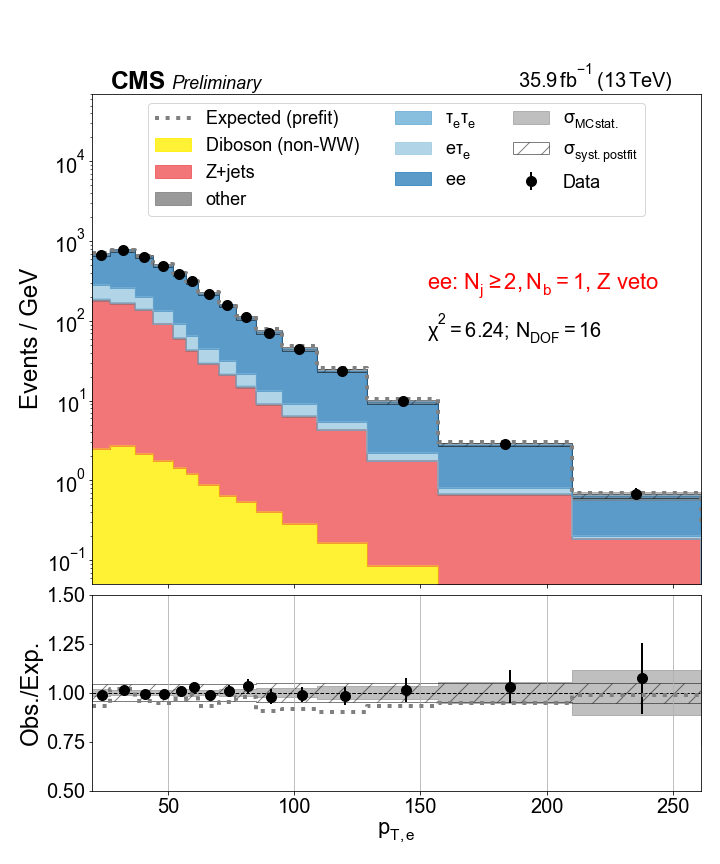
\includegraphics[width=0.4\textwidth]{chapters/Analysis/sectionStatisticalAnalysis/figures/fit/ee_cat_gt2_eq1_b}
    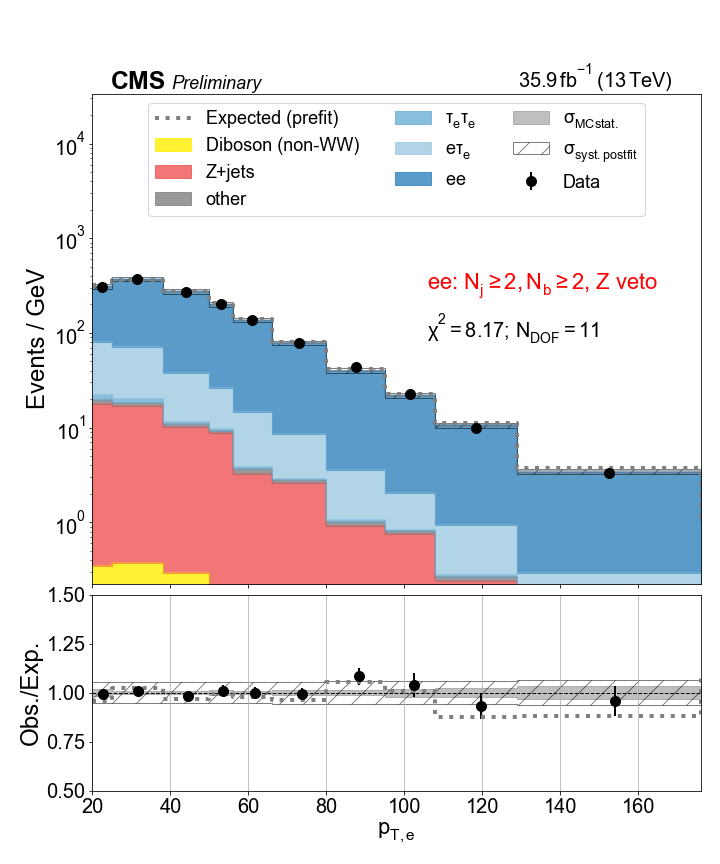
\includegraphics[width=0.4\textwidth]{chapters/Analysis/sectionStatisticalAnalysis/figures/fit/ee_cat_gt2_gt2_b}

    \caption{Templates used as inputs to the MLE fit for the $ee$ categories.}
    \label{fig:fits_templates_ee}
\end{figure}

\begin{figure}[htb!]
    \centering
    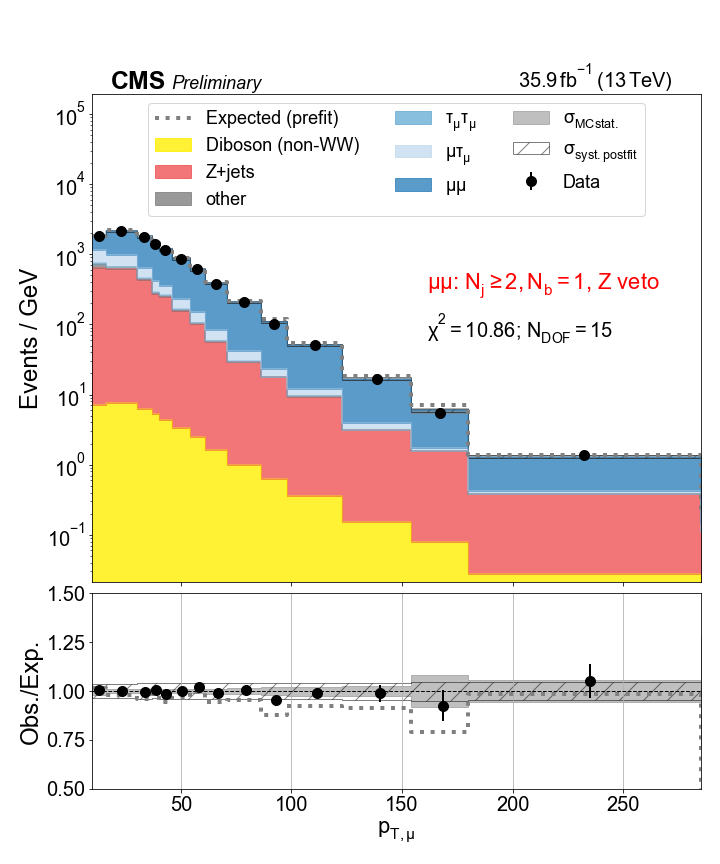
\includegraphics[width=0.4\textwidth]{chapters/Analysis/sectionStatisticalAnalysis/figures/fit/mumu_cat_gt2_eq1_b}
    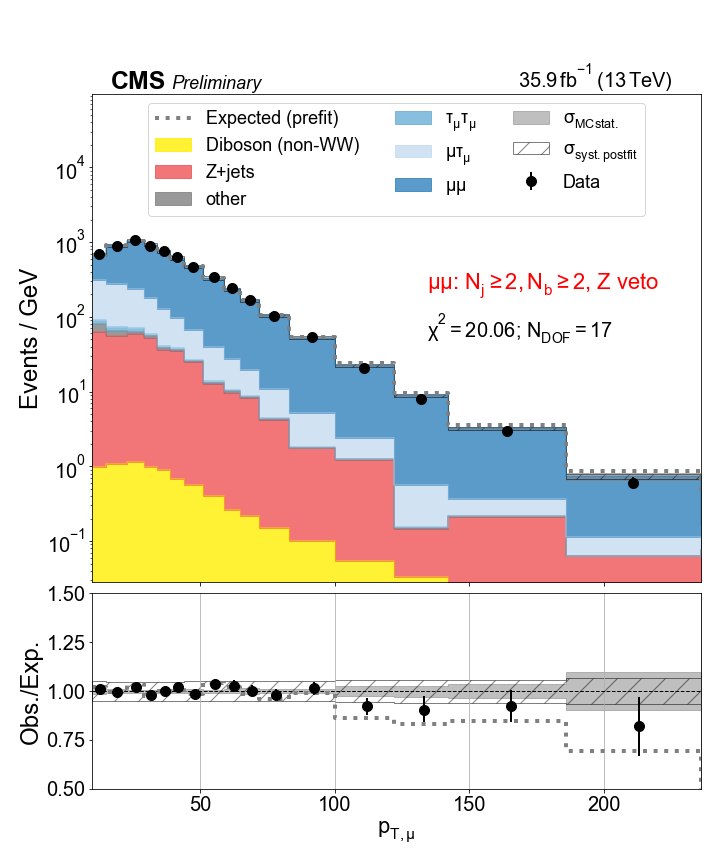
\includegraphics[width=0.4\textwidth]{chapters/Analysis/sectionStatisticalAnalysis/figures/fit/mumu_cat_gt2_gt2_b}

    \caption{Templates used as inputs to the MLE fit for the $\mu\mu$ categories.}
    \label{fig:fits_templates_mumu}
\end{figure}

\begin{figure}[htb!]
    \centering
    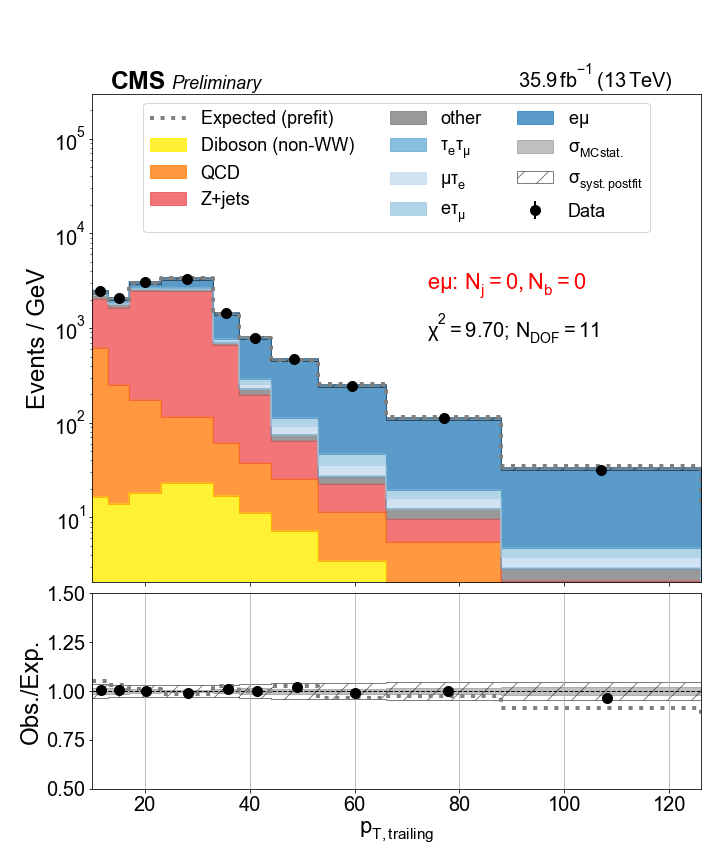
\includegraphics[width=0.3\textwidth]{chapters/Analysis/sectionStatisticalAnalysis/figures/fit/emu_cat_eq0_eq0_a}
    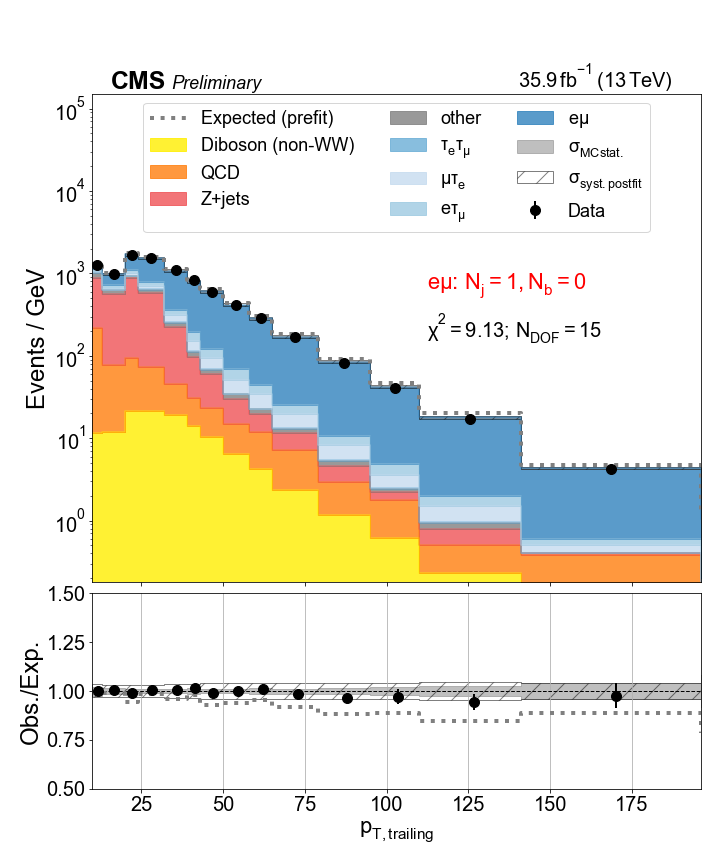
\includegraphics[width=0.3\textwidth]{chapters/Analysis/sectionStatisticalAnalysis/figures/fit/emu_cat_eq1_eq0_a}
    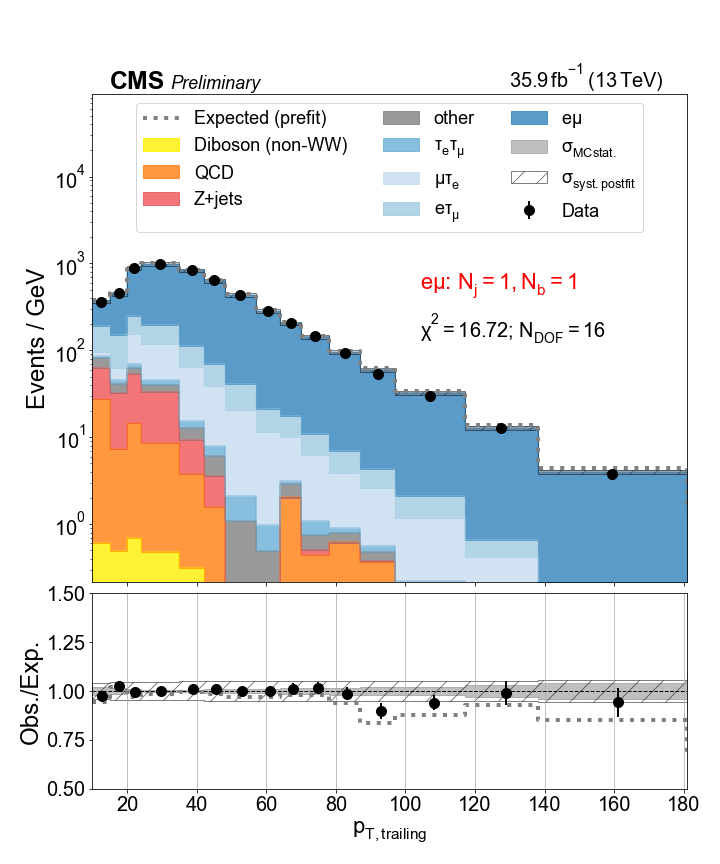
\includegraphics[width=0.3\textwidth]{chapters/Analysis/sectionStatisticalAnalysis/figures/fit/emu_cat_eq1_eq1_a}

    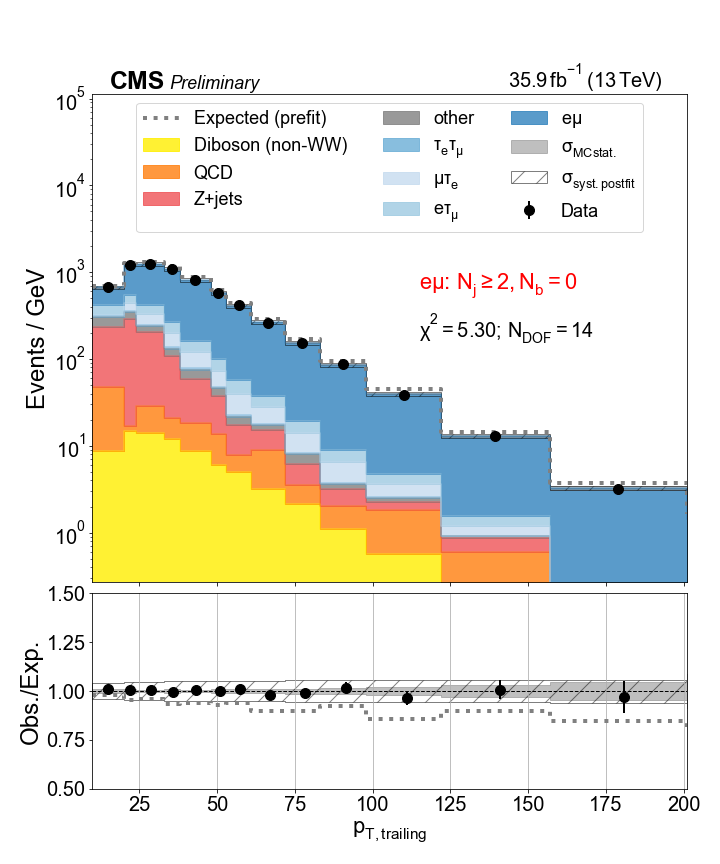
\includegraphics[width=0.3\textwidth]{chapters/Analysis/sectionStatisticalAnalysis/figures/fit/emu_cat_gt2_eq0}
    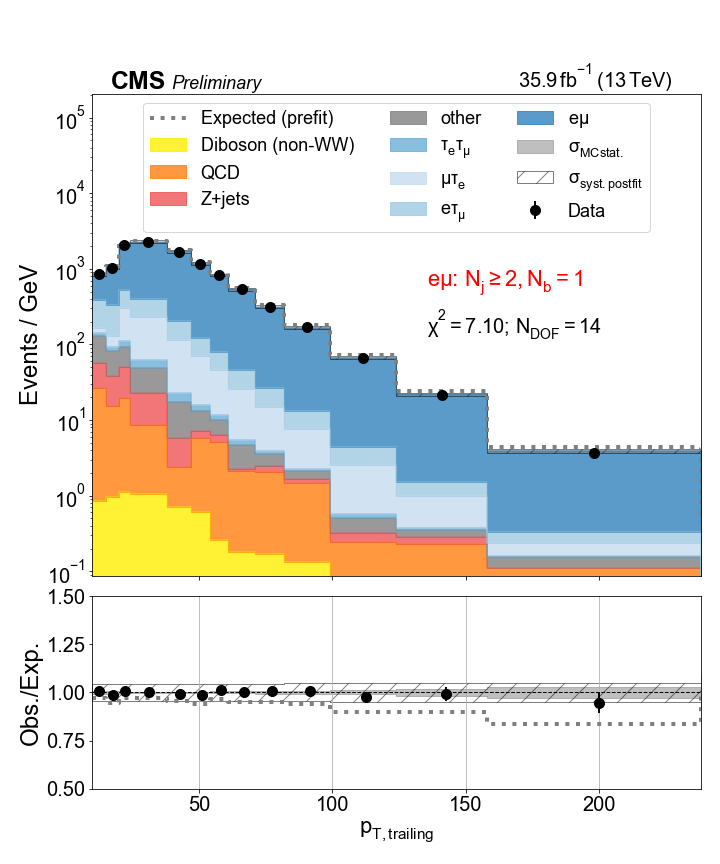
\includegraphics[width=0.3\textwidth]{chapters/Analysis/sectionStatisticalAnalysis/figures/fit/emu_cat_gt2_eq1_a}
    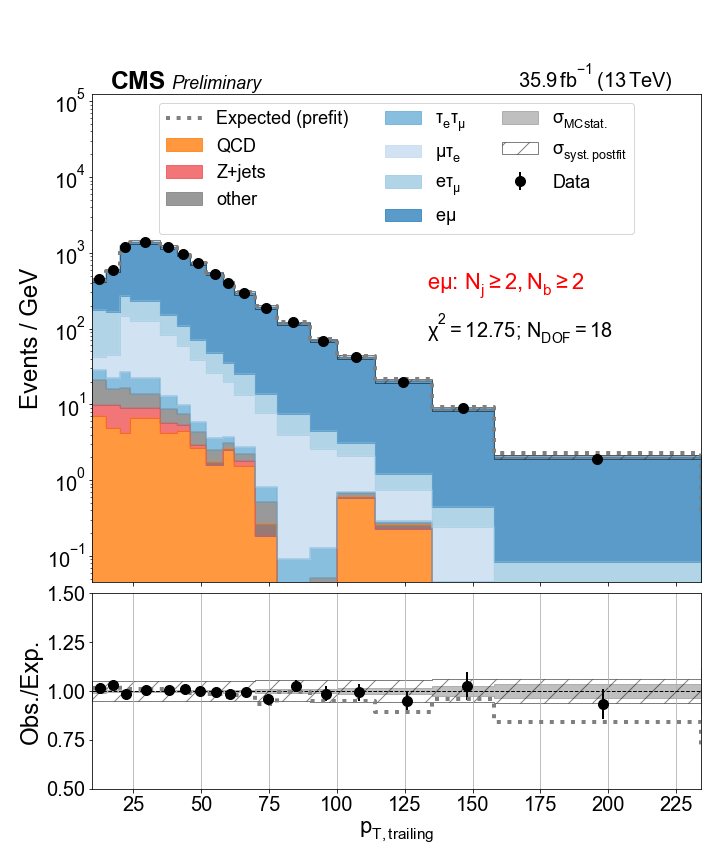
\includegraphics[width=0.3\textwidth]{chapters/Analysis/sectionStatisticalAnalysis/figures/fit/emu_cat_gt2_gt2_a}
    \caption{Templates used as inputs to the MLE fit for the $e\mu$
    category.}
    \label{fig:fits_templates_emu}
\end{figure}

\begin{figure}[htb!]
    \centering
    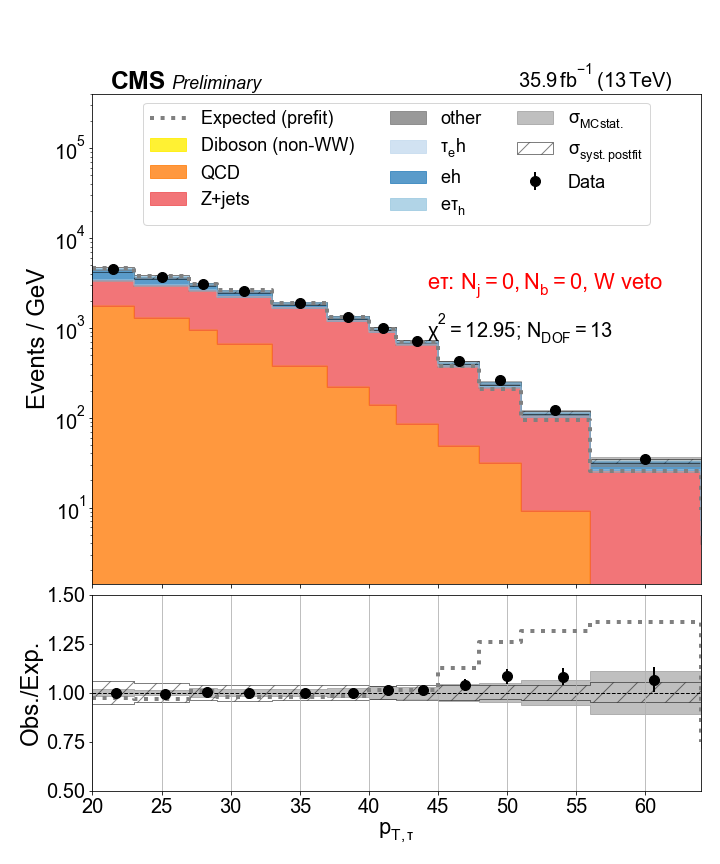
\includegraphics[width=0.24\textwidth]{chapters/Analysis/sectionStatisticalAnalysis/figures/fit/etau_cat_eq0_eq0}
    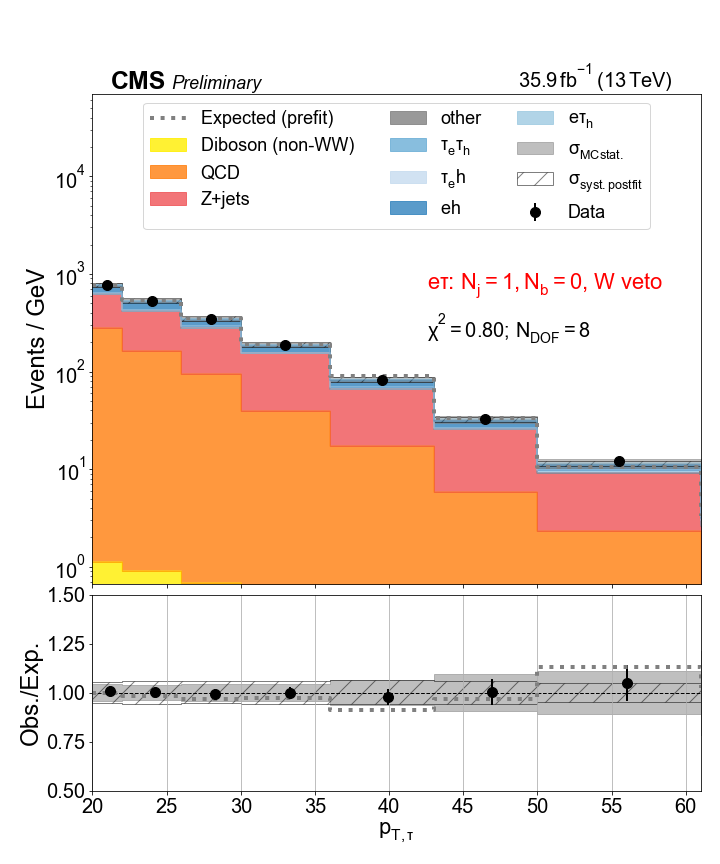
\includegraphics[width=0.24\textwidth]{chapters/Analysis/sectionStatisticalAnalysis/figures/fit/etau_cat_eq1_eq0}
    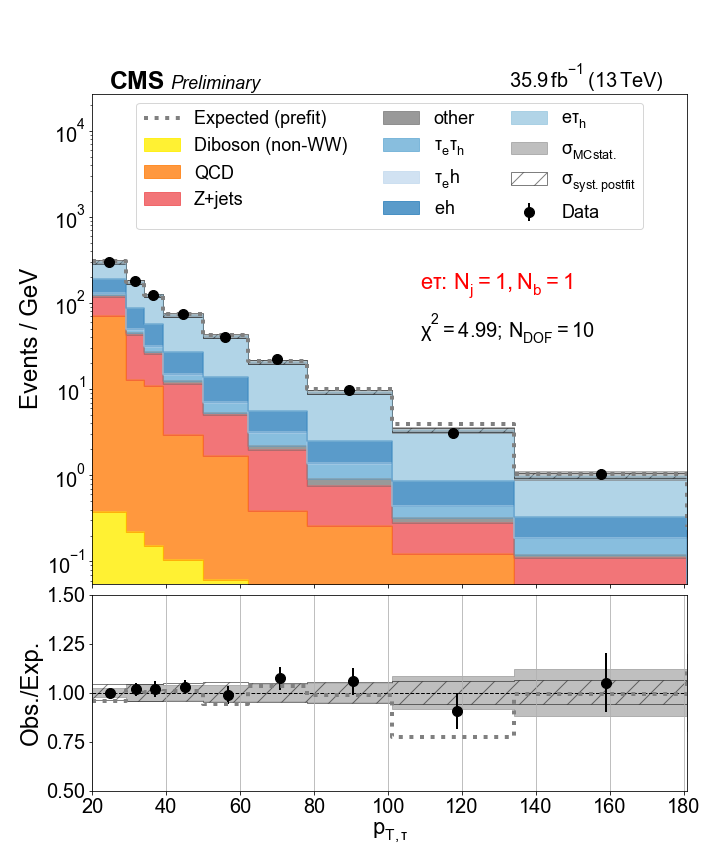
\includegraphics[width=0.24\textwidth]{chapters/Analysis/sectionStatisticalAnalysis/figures/fit/etau_cat_eq1_eq1}
    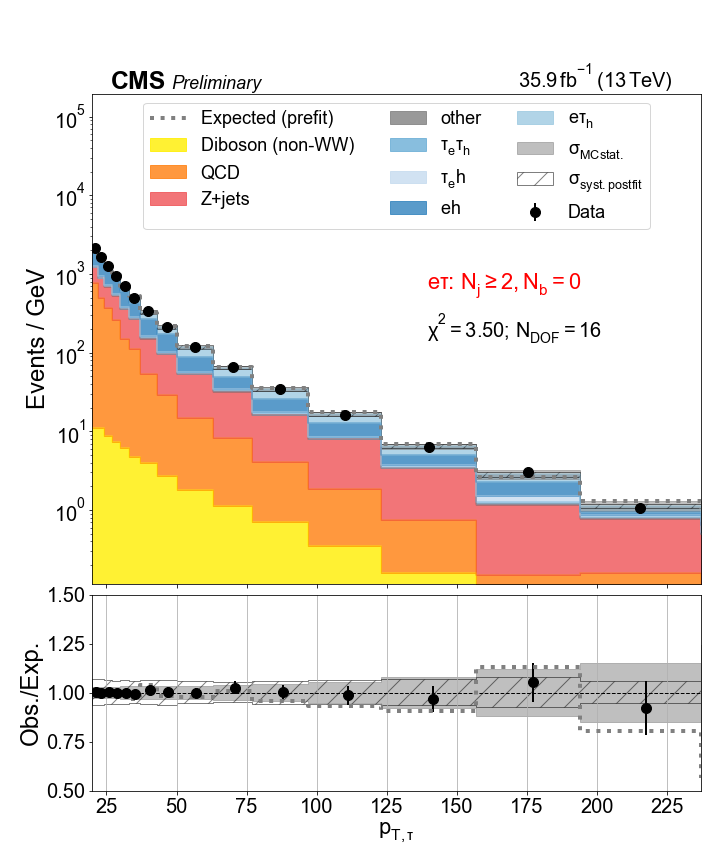
\includegraphics[width=0.24\textwidth]{chapters/Analysis/sectionStatisticalAnalysis/figures/fit/etau_cat_gt2_eq0}

    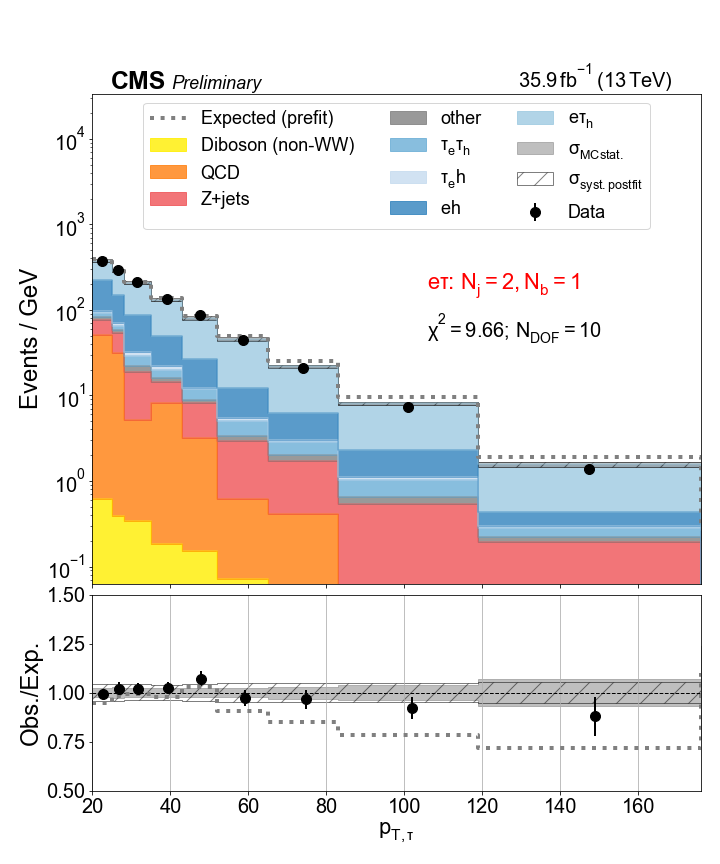
\includegraphics[width=0.24\textwidth]{chapters/Analysis/sectionStatisticalAnalysis/figures/fit/etau_cat_eq2_eq1}
    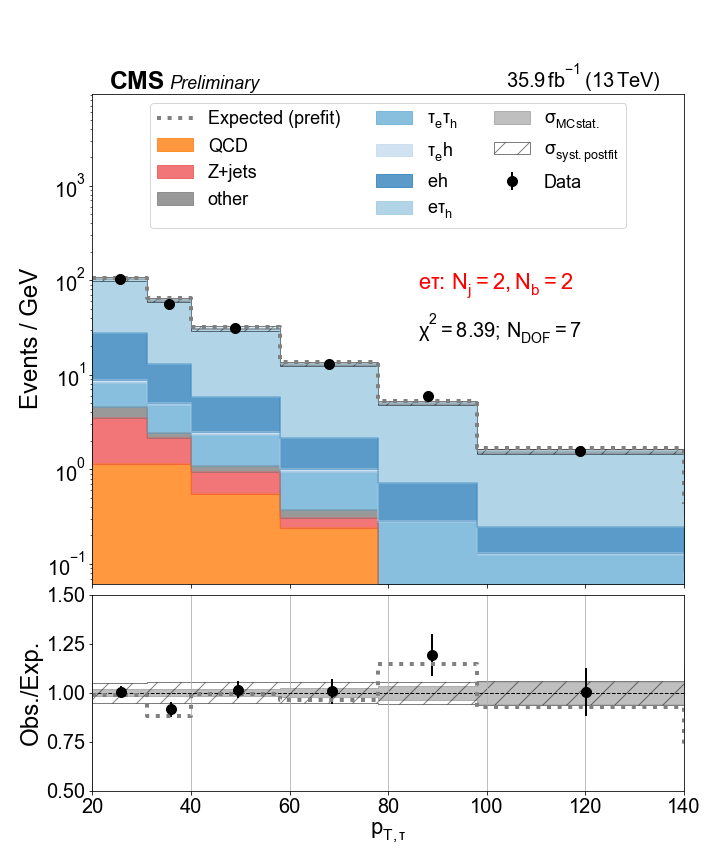
\includegraphics[width=0.24\textwidth]{chapters/Analysis/sectionStatisticalAnalysis/figures/fit/etau_cat_eq2_eq2}
    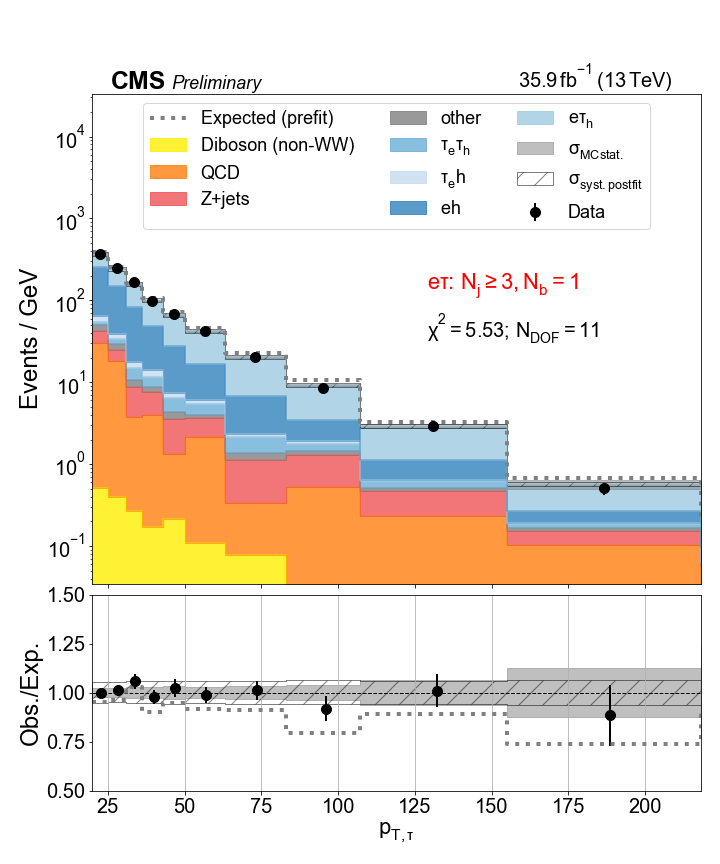
\includegraphics[width=0.24\textwidth]{chapters/Analysis/sectionStatisticalAnalysis/figures/fit/etau_cat_gt3_eq1}
    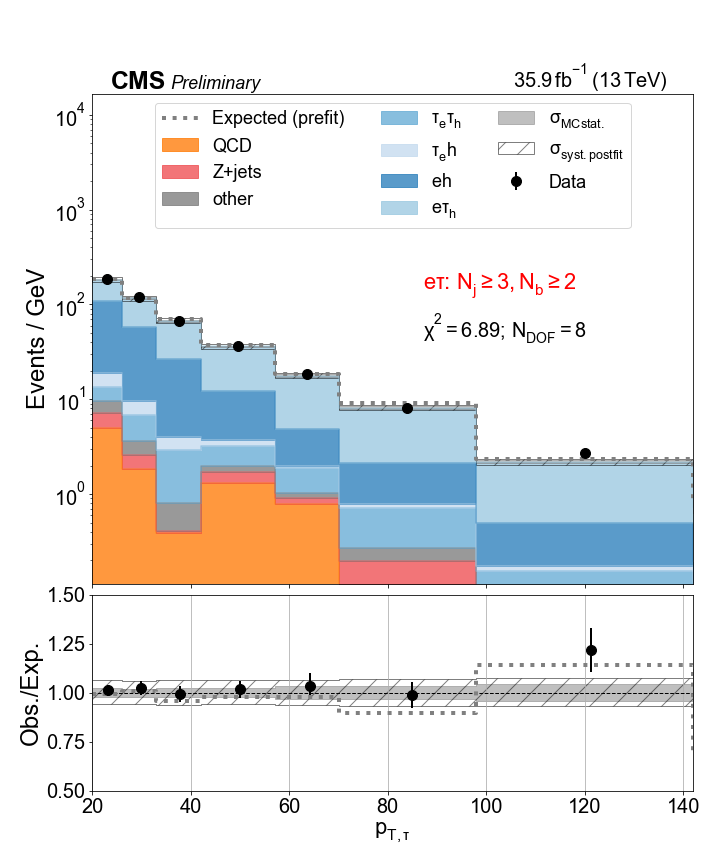
\includegraphics[width=0.24\textwidth]{chapters/Analysis/sectionStatisticalAnalysis/figures/fit/etau_cat_gt3_gt2}
    \caption{Templates used as inputs to the MLE fit for the $e\tau$
    category.}
    \label{fig:fits_templates_etau}
\end{figure}

\begin{figure}[htb!]
    \centering
    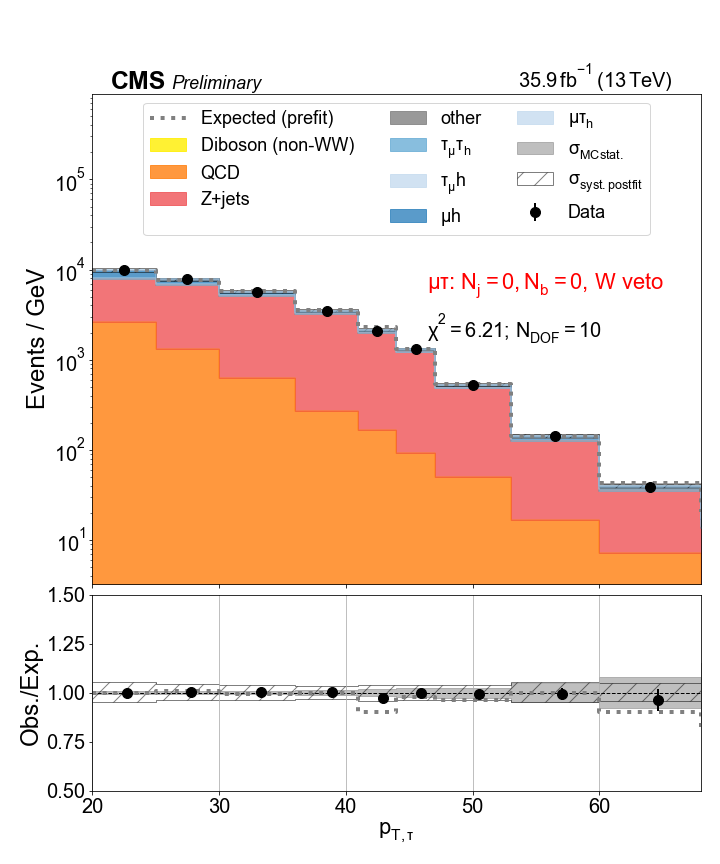
\includegraphics[width=0.24\textwidth]{chapters/Analysis/sectionStatisticalAnalysis/figures/fit/mutau_cat_eq0_eq0}
    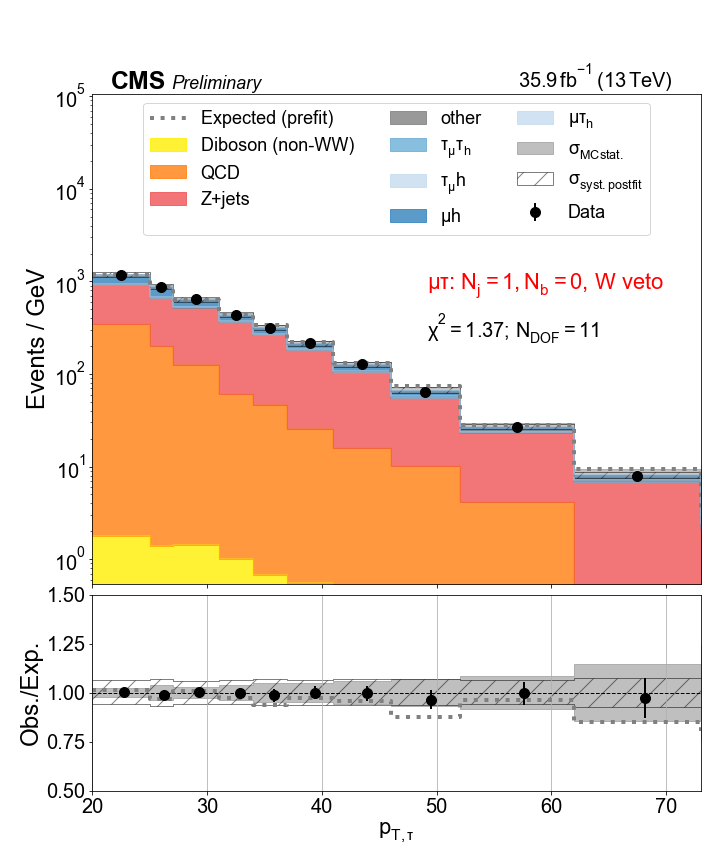
\includegraphics[width=0.24\textwidth]{chapters/Analysis/sectionStatisticalAnalysis/figures/fit/mutau_cat_eq1_eq0}
    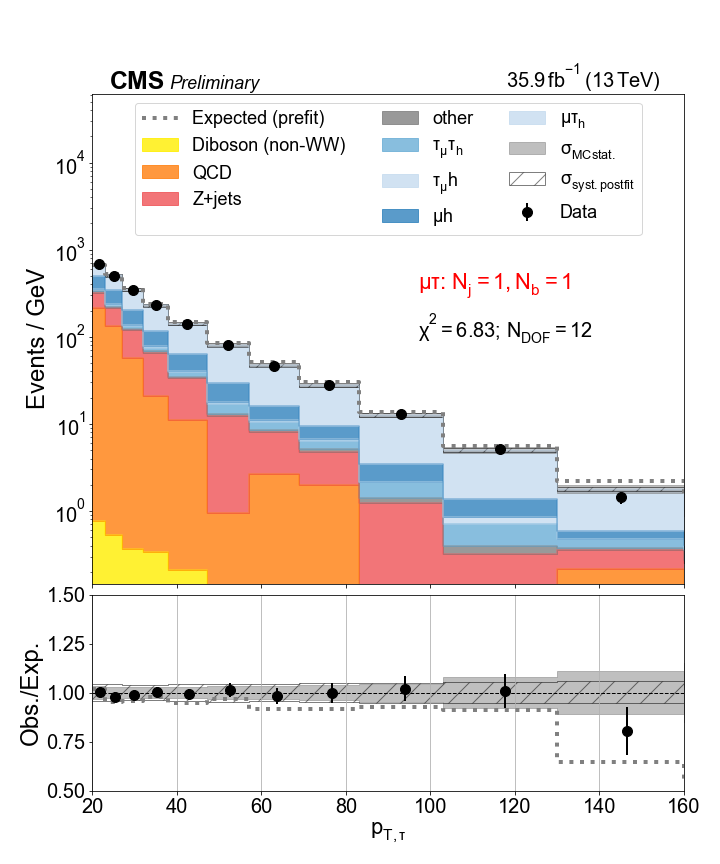
\includegraphics[width=0.24\textwidth]{chapters/Analysis/sectionStatisticalAnalysis/figures/fit/mutau_cat_eq1_eq1}
    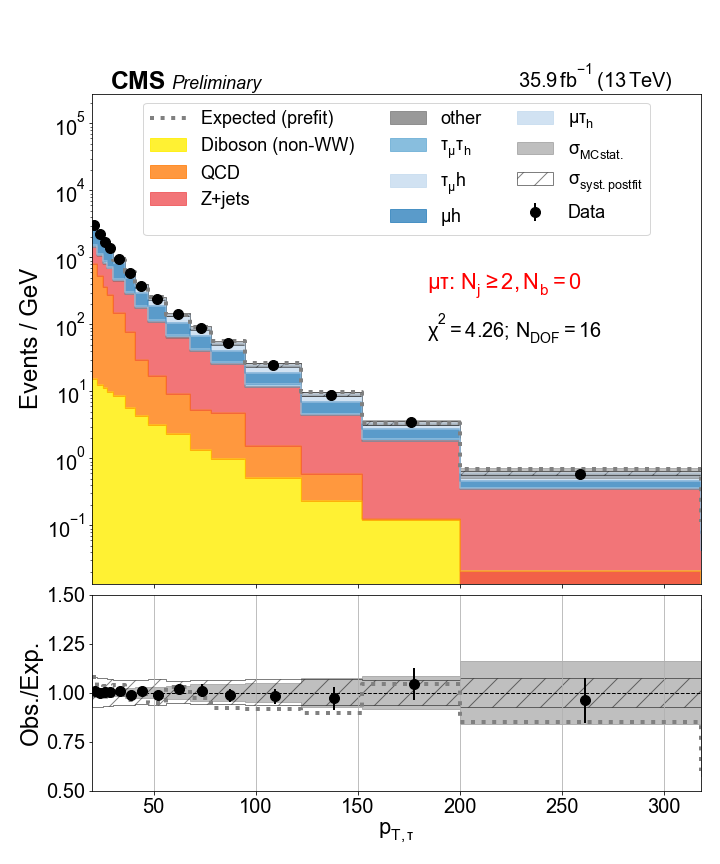
\includegraphics[width=0.24\textwidth]{chapters/Analysis/sectionStatisticalAnalysis/figures/fit/mutau_cat_gt2_eq0}

    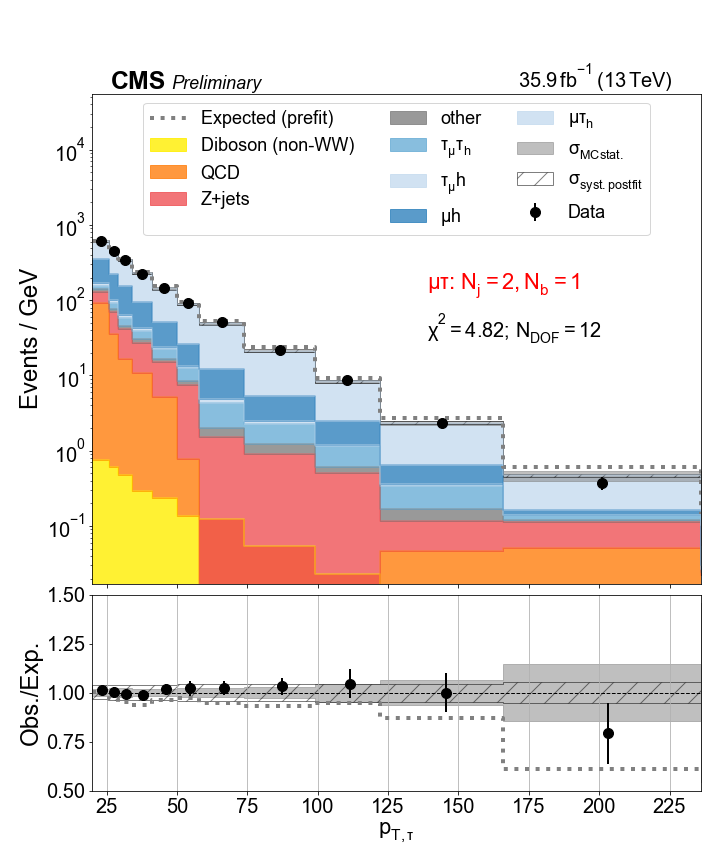
\includegraphics[width=0.24\textwidth]{chapters/Analysis/sectionStatisticalAnalysis/figures/fit/mutau_cat_eq2_eq1}
    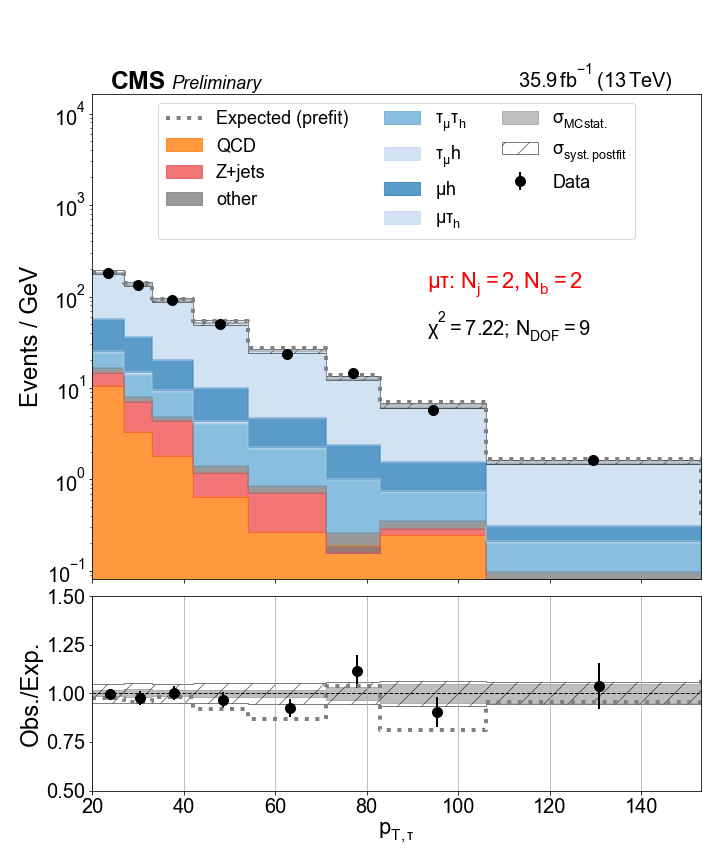
\includegraphics[width=0.24\textwidth]{chapters/Analysis/sectionStatisticalAnalysis/figures/fit/mutau_cat_eq2_eq2}
    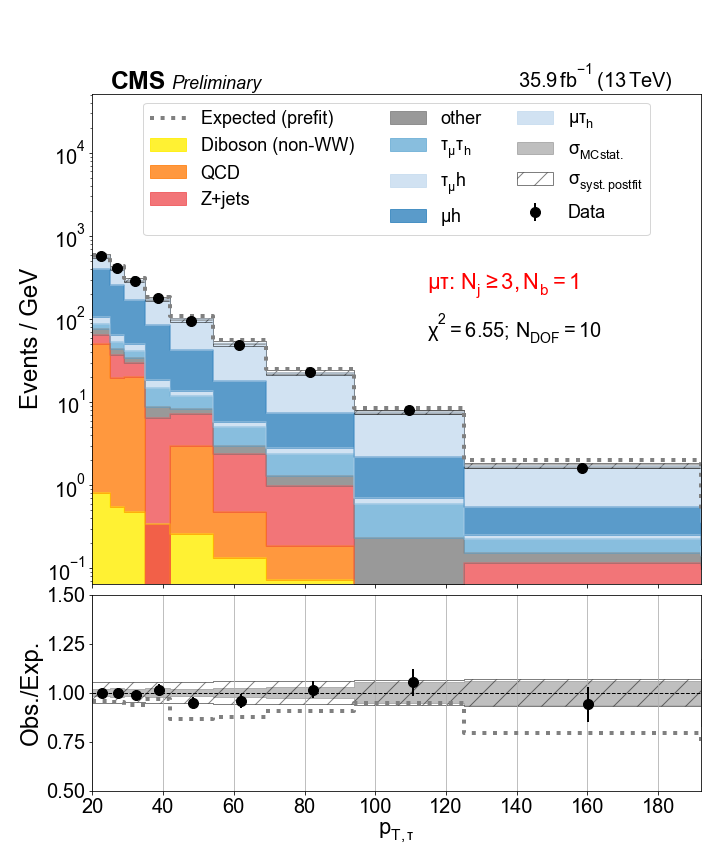
\includegraphics[width=0.24\textwidth]{chapters/Analysis/sectionStatisticalAnalysis/figures/fit/mutau_cat_gt3_eq1}
    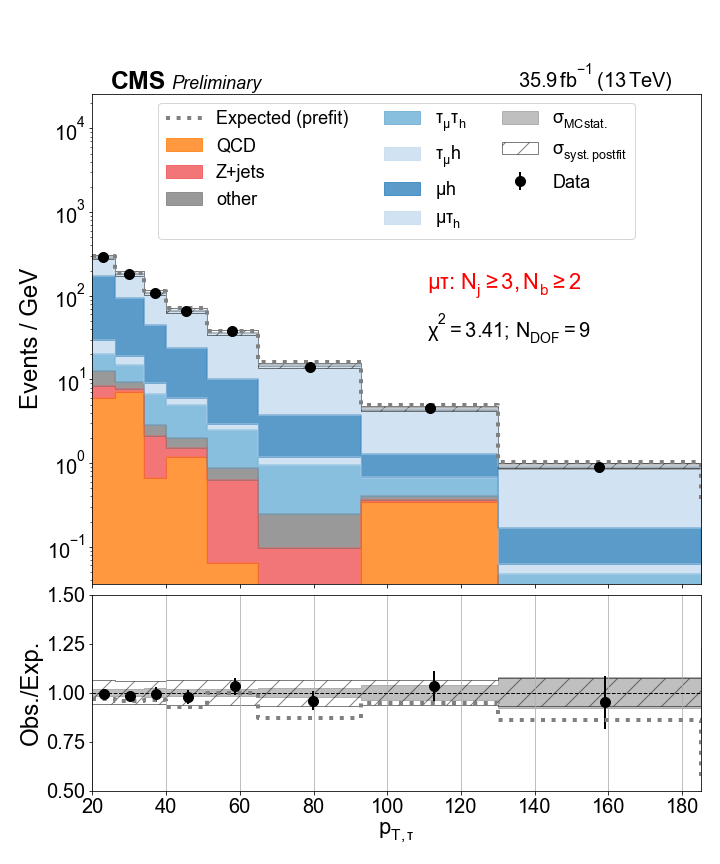
\includegraphics[width=0.24\textwidth]{chapters/Analysis/sectionStatisticalAnalysis/figures/fit/mutau_cat_gt3_gt2}
    \caption{Templates used as inputs to the MLE fit for the $\mu\tau$
    category.}
    \label{fig:fits_templates_mutau}
\end{figure}


\begin{figure}[htb!]
    \centering
    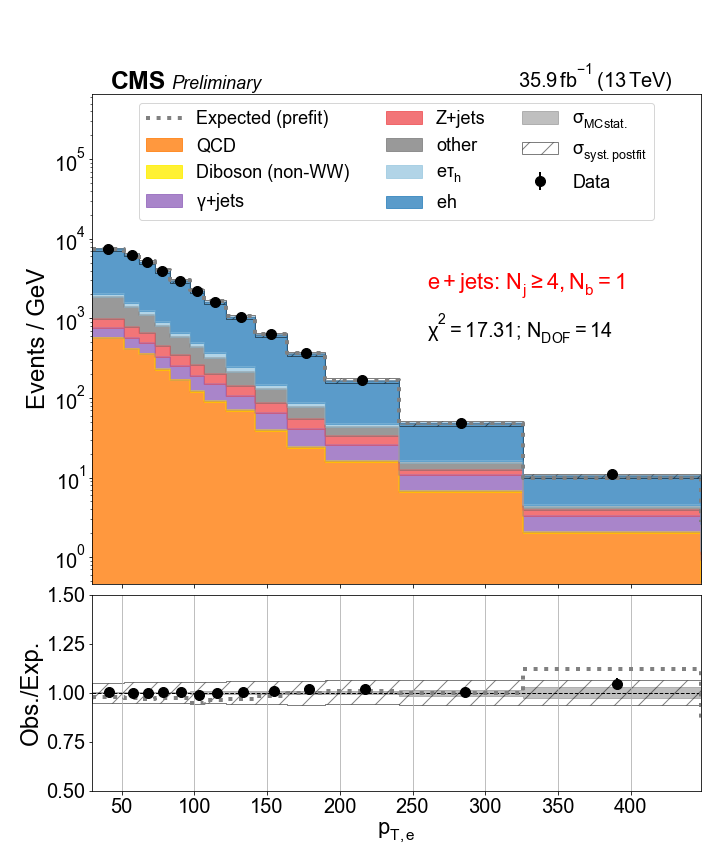
\includegraphics[width=0.4\textwidth]{chapters/Analysis/sectionStatisticalAnalysis/figures/fit/ejet_cat_gt4_eq1}
    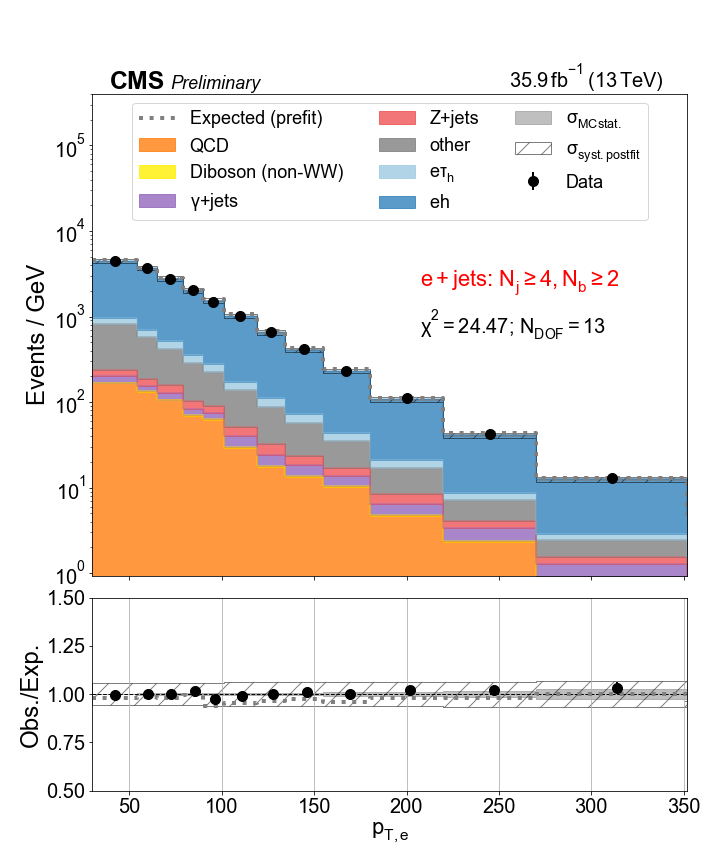
\includegraphics[width=0.4\textwidth]{chapters/Analysis/sectionStatisticalAnalysis/figures/fit/ejet_cat_gt4_gt2}
    \caption{Templates used as inputs to the MLE fit for the $eh$ categories.}
    \label{fig:mle_templates_e4j}
\end{figure}

\begin{figure}[htb!]
    \centering
    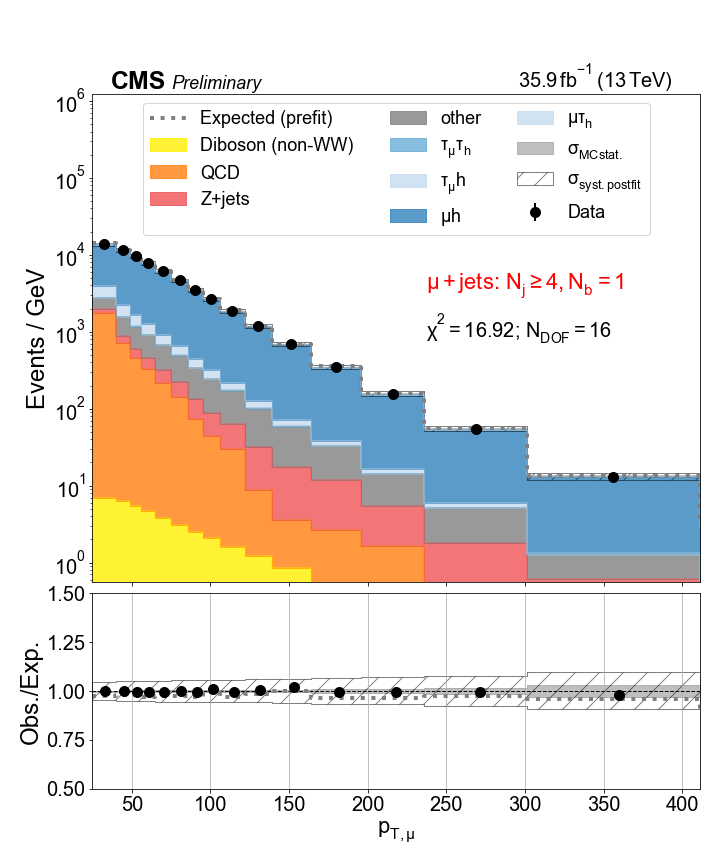
\includegraphics[width=0.4\textwidth]{chapters/Analysis/sectionStatisticalAnalysis/figures/fit/mujet_cat_gt4_eq1}
    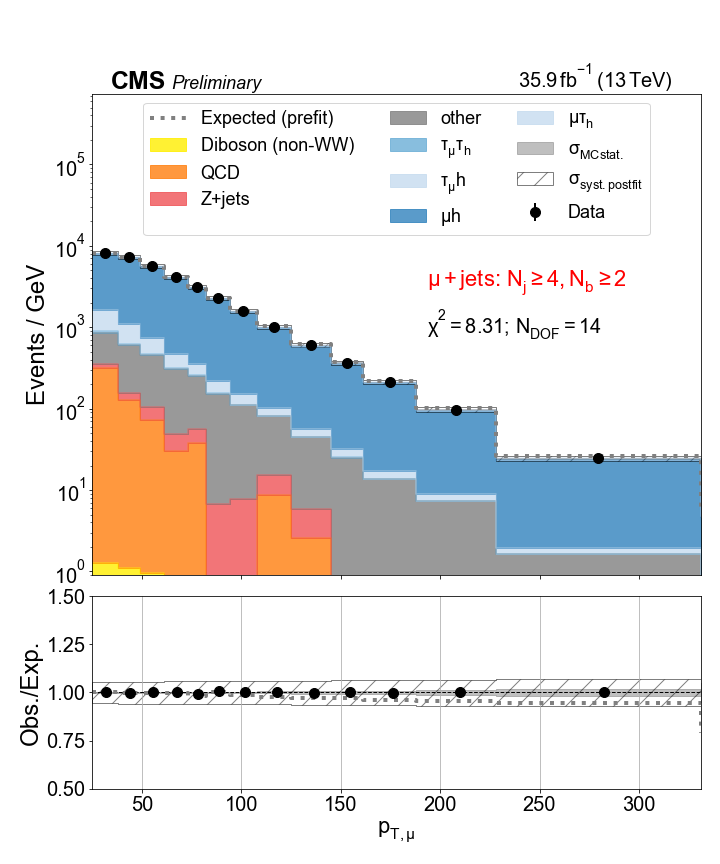
\includegraphics[width=0.4\textwidth]{chapters/Analysis/sectionStatisticalAnalysis/figures/fit/mujet_cat_gt4_gt2}
    \caption{Templates used as inputs to the MLE fit for the $\mu h$ categories.}
    \label{fig:mle_templates_mu4j}
\end{figure}


Effectively, this parameterizes the efficiency matrix in
equation~\ref{eq:eff_matrix} by the observables listed above, the number
of jets, and the number of b tags.  Having constructed the data model,
the negative log likelihood can be constructed,
\begin{equation}
\label{eq:nll}
\mathcal{L}(\boldsymbol{\beta}) = \sum_{\mathrm{i\in bin}} -y_{i}\ln
f_{i}(\boldsymbol{\beta}) + f_{i}(\boldsymbol{\beta}),
\end{equation}

where $y_{i}$ is the data yield in bin $i$.  The predicted yields,
$f_{i}$ are a linear combination of the various signal and background
templates, 
\begin{equation}
    f(\boldsymbol{\beta}) = \sum_{\rm s \in
    sig.}s(\boldsymbol{\beta}) + \sum_{\rm b\in bg} b.
\end{equation}

The signal term, $s_{i}$ is as written in eq.~\ref{eq:data_model}, i.e.,
a mixture of the 21 possible decay modes and the amplitudes for each
term are products of the branching fractions function of the W branching
fractions, $\boldsymbol{\beta}$.  



\subsubsection{Assessment of systematic uncertainties using nuisance parameters}
\label{sec:analysis:shape_syst}

The shape analysis accounts for the effects of various sources of
systematic uncertainties by incorporating nuisance parameters into the
fit~\cite{Conway:2011in}.  The individual sources of systematics
uncertainties are described in section~\ref{sec:analysis:systematics}.  This
approach to the systematic uncertainties has the benefit that all
correlations between the various nuisance parameters that exist in the
model definition are accounted for when the regression is carried
out.  In some cases, the nuisance parameters can become constrained by
the fit.  Additionally, it is straight forward to incorporate auxiliary
control regions ($\PZ\rightarrow\tau\tau$) to improve the constraints on
background normalizations or uncertainty on the modeling of physics
objects in simulation.

The modification to the objective function follows the approach
recommended by Conway, i.e., adding additional terms,
$\pi(\boldsymbol{\theta})$, to the cost function to account for the
priors on the nuisance parameters, $\theta$,
\begin{equation}
\label{eq:nll_full}
    \mathcal{L}(\boldsymbol{\beta}, \boldsymbol{\theta}) =
    \sum_{\mathrm{i \in bins}} \left[-y_{i}\ln
    f_{i}(\boldsymbol{\beta}, \boldsymbol{\theta}) +
    f_{i}(\boldsymbol{\beta}, \boldsymbol{\theta})\right] +
    \sum_{\theta \in \boldsymbol{\theta}}\pi(\theta).
\end{equation}

The nuisance parameters are treated either as normalization parameters
(multiplicative factors which are bin independent) or shape nuisance
parameters which vary depending on the bin they are applied to.  In the
latter case, morphing templates are generated for the cases that the
nuisance parameters are shifted up and down by one standard deviation.
The details for each source of systematic uncertainty is described in
section~\ref{sec:analysis:systematics}.  In practical terms, normalization
parameters are incorporated as they would appear in the explicit
construction of the data model (e.g., in place of a fixed value for the
$\mathcal{L}$ or a production cross section), whereas shape nuisances
appear as modifications to the bin contents of the templates.  A
quadratic morphing of the bin content as a function of a nuisance
parameter is used for values $\theta \in [-1, 1]$,
\begin{equation}
\label{eq:shape_param}
    \epsilon = \frac{\theta(\theta - 1)}{2}\epsilon^{-} - (\theta - 1)(\theta +
    1)\epsilon^{0} + \frac{\theta(\theta + 1)}{2}\epsilon^{+},
\end{equation}

with $\epsilon^{0}$ corresponding to the nominal efficiency in a given
bin, and $\epsilon^{-}$ and $\epsilon^{+}$ correspond to the down and up
variations of the relevant source of uncertainty.  It is useful to
rewrite this expression so the dependence on $\theta$ is clearer,
\begin{align}
    \Delta\epsilon &= \epsilon - \epsilon^{0} \\
     &= \frac{\theta^{2}}{2}(\Delta\epsilon^{+} + \Delta\epsilon^{-}) 
     + \frac{\theta}{2}(\Delta\epsilon^{+} - \Delta\epsilon^{-}) \\
     &= \frac{\Delta_{+}}{2}\theta^{2}  + \frac{\Delta_{-}}{2}\theta
\end{align}

where,
\begin{equation}
    \Delta\epsilon^{\pm} = \epsilon^{\pm} - \epsilon^{0}, \quad \Delta_{\pm} = \Delta\epsilon^{+} \pm \Delta\epsilon^{-} .
\end{equation}

It is worth noting that in the circumstance that the variation in yield
is symmetric about nominal value as a function of $\theta$, the
quadratic term becomes unimportant.  Outside the range $[-1, 1]$, the
bin content varies linearly with the value of $\theta$,
\begin{equation}
    \Delta\epsilon = 
    \begin{cases}
            (\Delta_{+} + \frac{\Delta_{-}}{2})\theta - \frac{\Delta_{+}}{2},
            & \text{if } \theta > 1 \\
            (-\Delta_{+} + \frac{\Delta_{-}}{2})\theta - \frac{\Delta_{+}}{2},
            & \text{if } \theta < -1
    \end{cases}
\end{equation}

This is derived by requiring that $\Delta\epsilon$ be continuous and
differentiable at the boundaries.  The total change to the predicted
efficiency is then the sum over all $\Delta\epsilon$, 
\begin{equation}
    \epsilon' = \epsilon^{0} + \sum_{\theta\in\boldsymbol{\theta}}\Delta\epsilon_{\theta}
\end{equation}

Nuisance parameters are assumed to be Gaussian constrained unless
otherwise noted,
\begin{equation}
    \pi(\theta) = e^{-\frac{(\theta_{0}^{2} -
    \hat{\theta}^{2})}{2\sigma_{\theta}^{2}}},
\end{equation}

where $\sigma_{\theta}$ is the uncertainty on parameter $\theta$ for
normalization uncertainties, and one for shape parameters (the specific
values of uncertainty is included in the morphing templates for
$\theta$).

The branching fraction estimates are determined by minimizing
equation~\ref{eq:nll_full} with respect to all parameters.  This is done
for all final state channels and b tag bins simultaneously which
accounts for correlations between common nuisance parameters and the W
branching fractions.

\subsubsection{MC statistics}
% \subsubsection{Systematic uncertainty due to limited MC statistics}

In addition to various sources of uncertainty associated with the
detector and with the modeling of physical processes, there is a
non-negligible uncertainty arising from the finite and limited
statistics of the simulated samples used to model the data.  Ideally,
the simulated samples would have $>5$ times the number of events
collected in data for each process.  This is generally not the case, and
in some cases, the number of simulated events is less than the number of
corresponding events collected in data.  With this in mind, the
Barlow-Beeston lite method is adopted to account for the resulting
uncertainty.  In brief, this entails introducing a n.p. for each bin in
the analysis that controls the normalization of that bin and is
constrained according to the variance associated with the statistics
of the simulated samples.  Because, these n.p. are to first order not
correlated across bins, they can be solved for analytically as described
in section 5 of Conway~\cite{Conway:2011in}.

% originally from the systematical uncertainty
This analysis relies heavily on simulated samples to estimate
backgrounds and the signal processes.  The number of events generated in
each MC sample is frequently limited so an additional uncertainty must
be assessed to account for this.  For the most part, it is not an issue
in the counting analysis, but it is still accounted for by varying the
MC templates within their statistical uncertainties and carrying out the
analysis.  For the shape analysis, the Barlow-Beeston
method~\cite{Amsler:2008zzb} is adopted.  This method includes an
intermediate step in the minimization of the NLL where the NLL is
minimized with respect to nuisance parameters associated with the
normalization of individual bins.  The nuisance parameters are allowed
to vary within the combined MC statistical uncertainty associated with the
bin.  The impact of this is particularly large where the normalization
of the Drell-Yan sample is concerned since the size of the simulated
sample is on the order of the number of events produced in data.



\subsubsection{Study of statistical bias of parameters}

It is desirable that the method produces an unbiased measurement of the
W branching fractions.  Even though it is not expected that bias should
arise, it is worth verifying this with a toy MC study.  This is carried
out by generating 10,000 pseudo-datasets from the nominal data model
templates with values of the branching fractions samples in the ranges
$\beta_{e}, \beta_{\mu}, \beta_{\tau} \in [0.1, 0.12]$ with $\beta_{h} =
1 - (\beta_{e} + \beta_{\mu} + \beta_{\tau})$.  For each of the 10,000
quadruplets, $\beta_{0}$ of branching fraction values, a pseudo-dataset
is generated accounting for poisson statistics of each individual signal
and background template, and the search procedure is carried out, i.e.,
equation~\ref{eq:nll} is minimized to determine $\hat{\beta}$.  From
this, the bias can be determined,
\begin{equation}
\label{eq:bias}
    \mathrm{bias} = \frac{\beta_{true} - \beta_{obs}}{\beta_{true}}.
\end{equation}

The results of this study are shown in figures~\ref{fig:bias_scan} and
\ref{fig:bias_test}.  The mean value of the bias shows no deviation from
zero within the variance.  There is also no indication that there is
a dependence of the bias on the true value of the branching fraction
used to generate the data.

\begin{figure}[htb!]
    \centering
    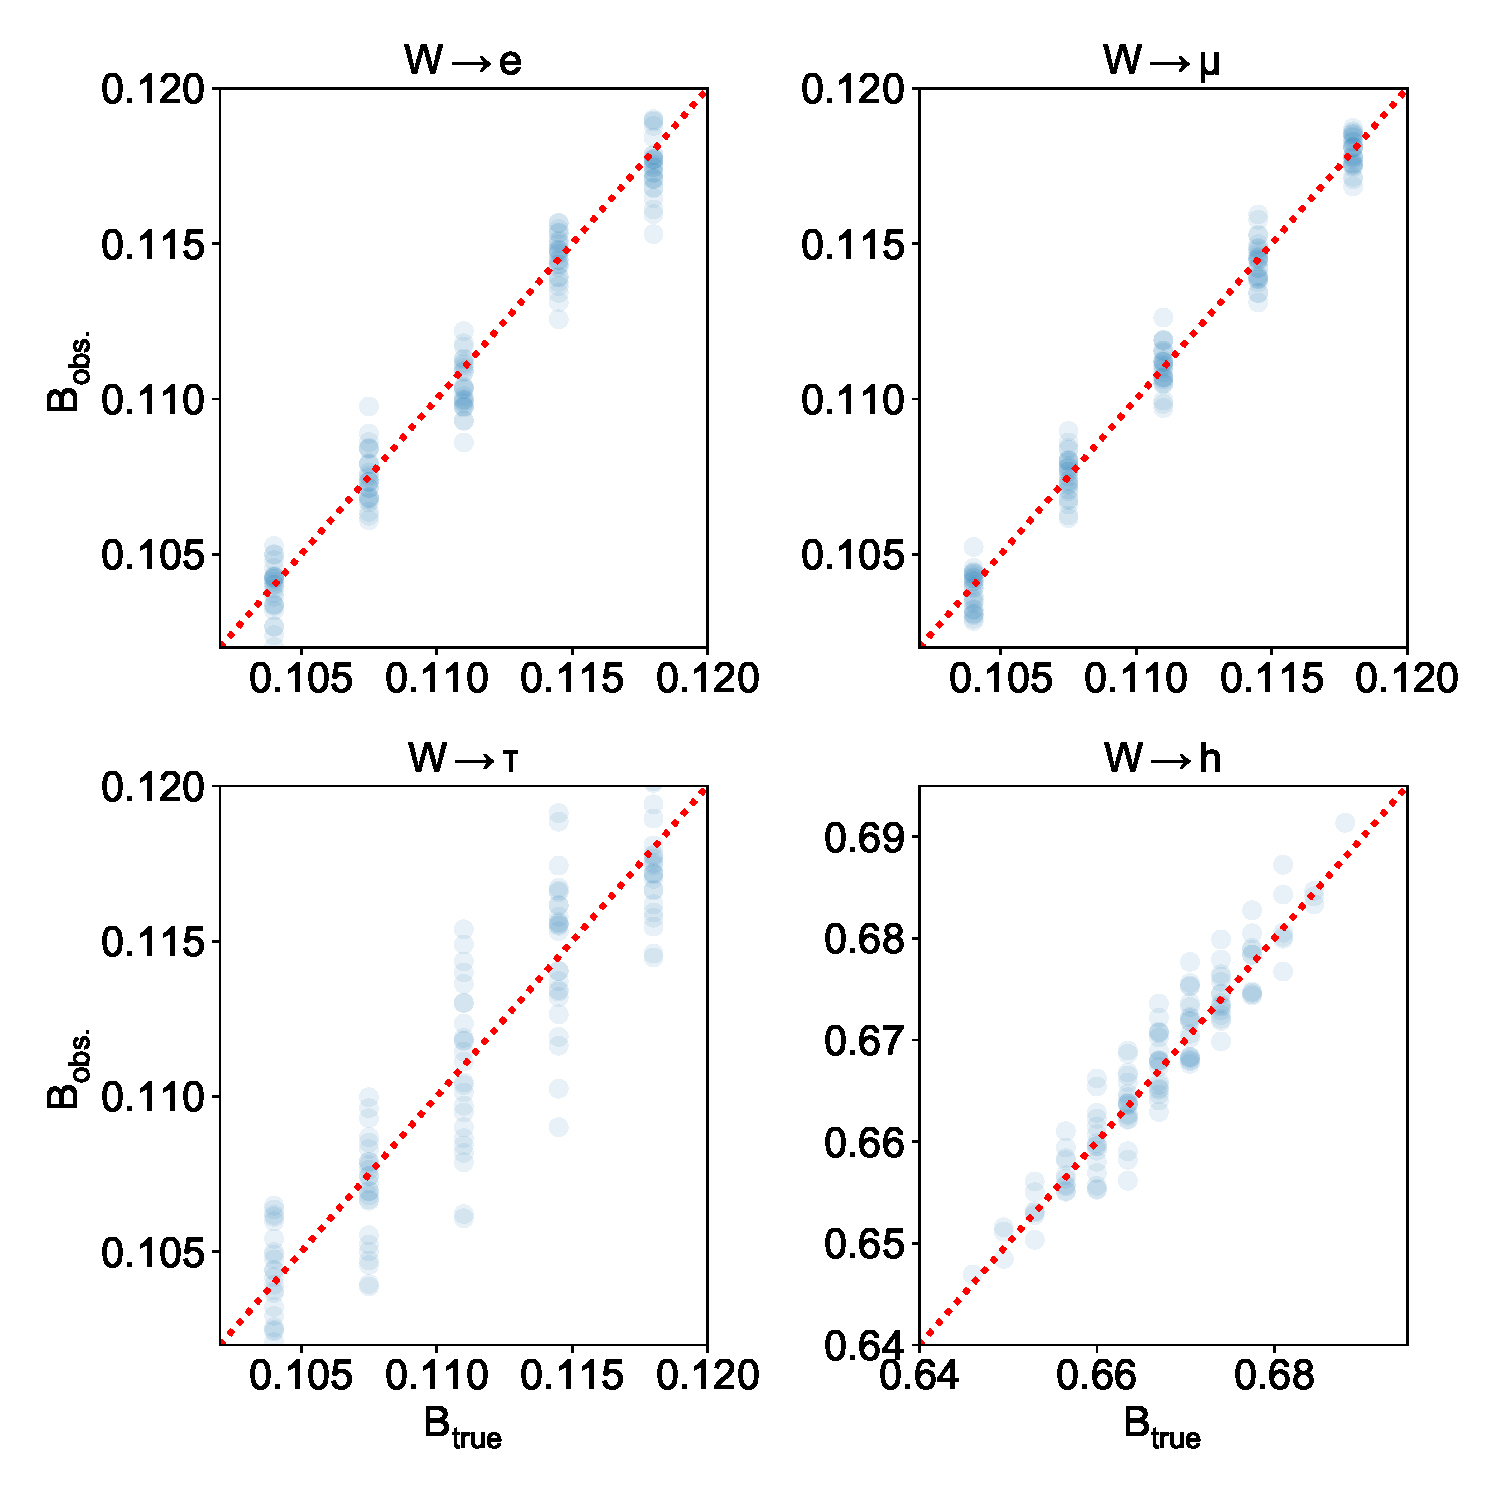
\includegraphics[width=0.8\textwidth]{chapters/Analysis/sectionStatisticalAnalysis/figures/beta_scan}
    \caption{Results of bias test showing the value of each of the four
    branching fractions determined from the fit versus the value used to
    generate the pseudo-dataset.  The red dashed line indicates a line
    of slope one passing throught the origin.}
    \label{fig:bias_scan}
\end{figure}

\begin{figure}[htb!]
    \centering
    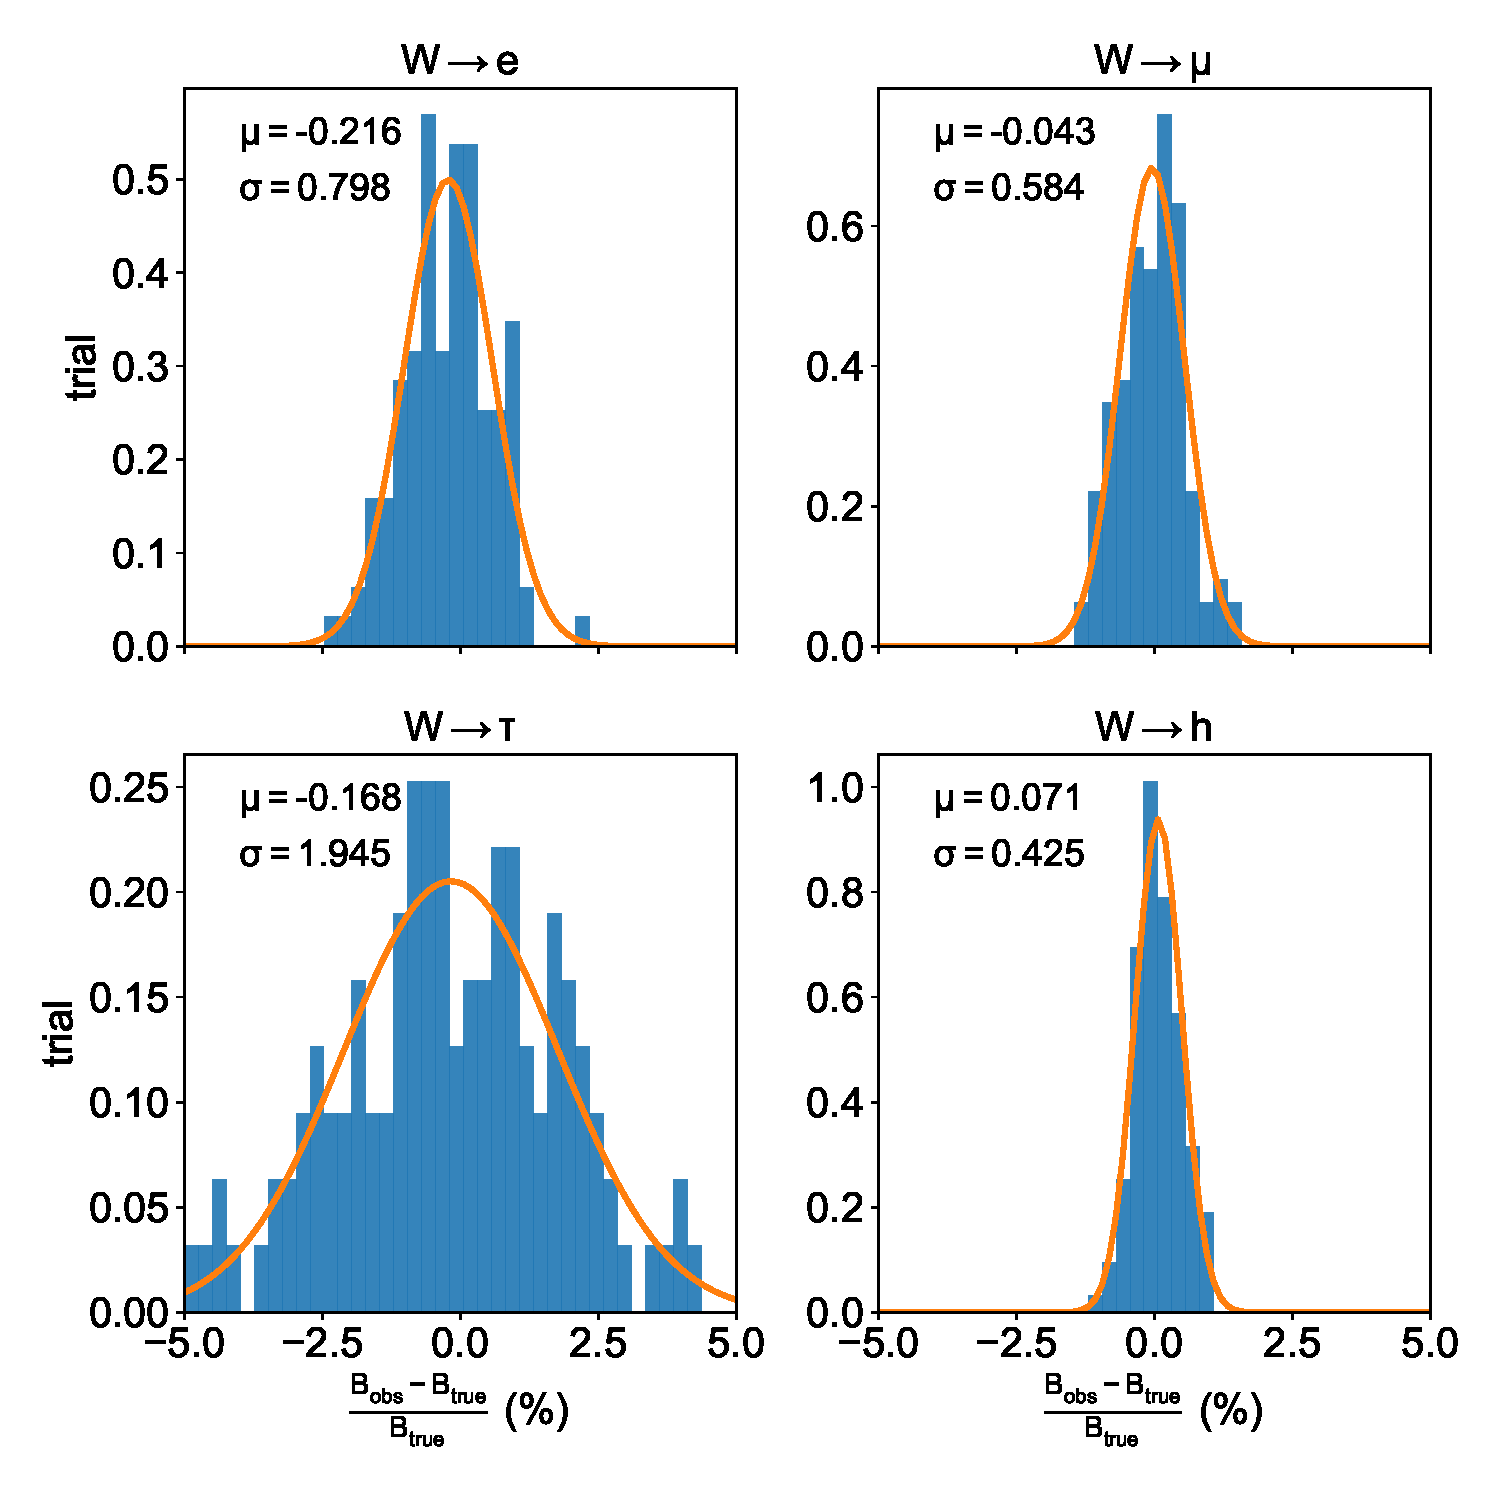
\includegraphics[width=0.8\textwidth]{chapters/Analysis/sectionStatisticalAnalysis/figures/beta_bias}
    \caption{Histogrammed values of the bias (defined in
    equation~\ref{eq:bias} measured for each of the scan points.  The
    values of $\mu$ and $\sigma$ denote the mean and standard error for
    each distribution.}
    \label{fig:bias_test}
\end{figure}

This study also allows for an independent estimation of the uncertainty
on each of the parameters.  The resulting uncertainties estimated from
the toy data are found to be close to the values calculated by carrying
out a numerical estimation of the NLL Hessian about its minimum.  This
comparison is shown in figure~\ref{fig:pulls_comparison}.

\begin{figure}[htb!]
    \centering
    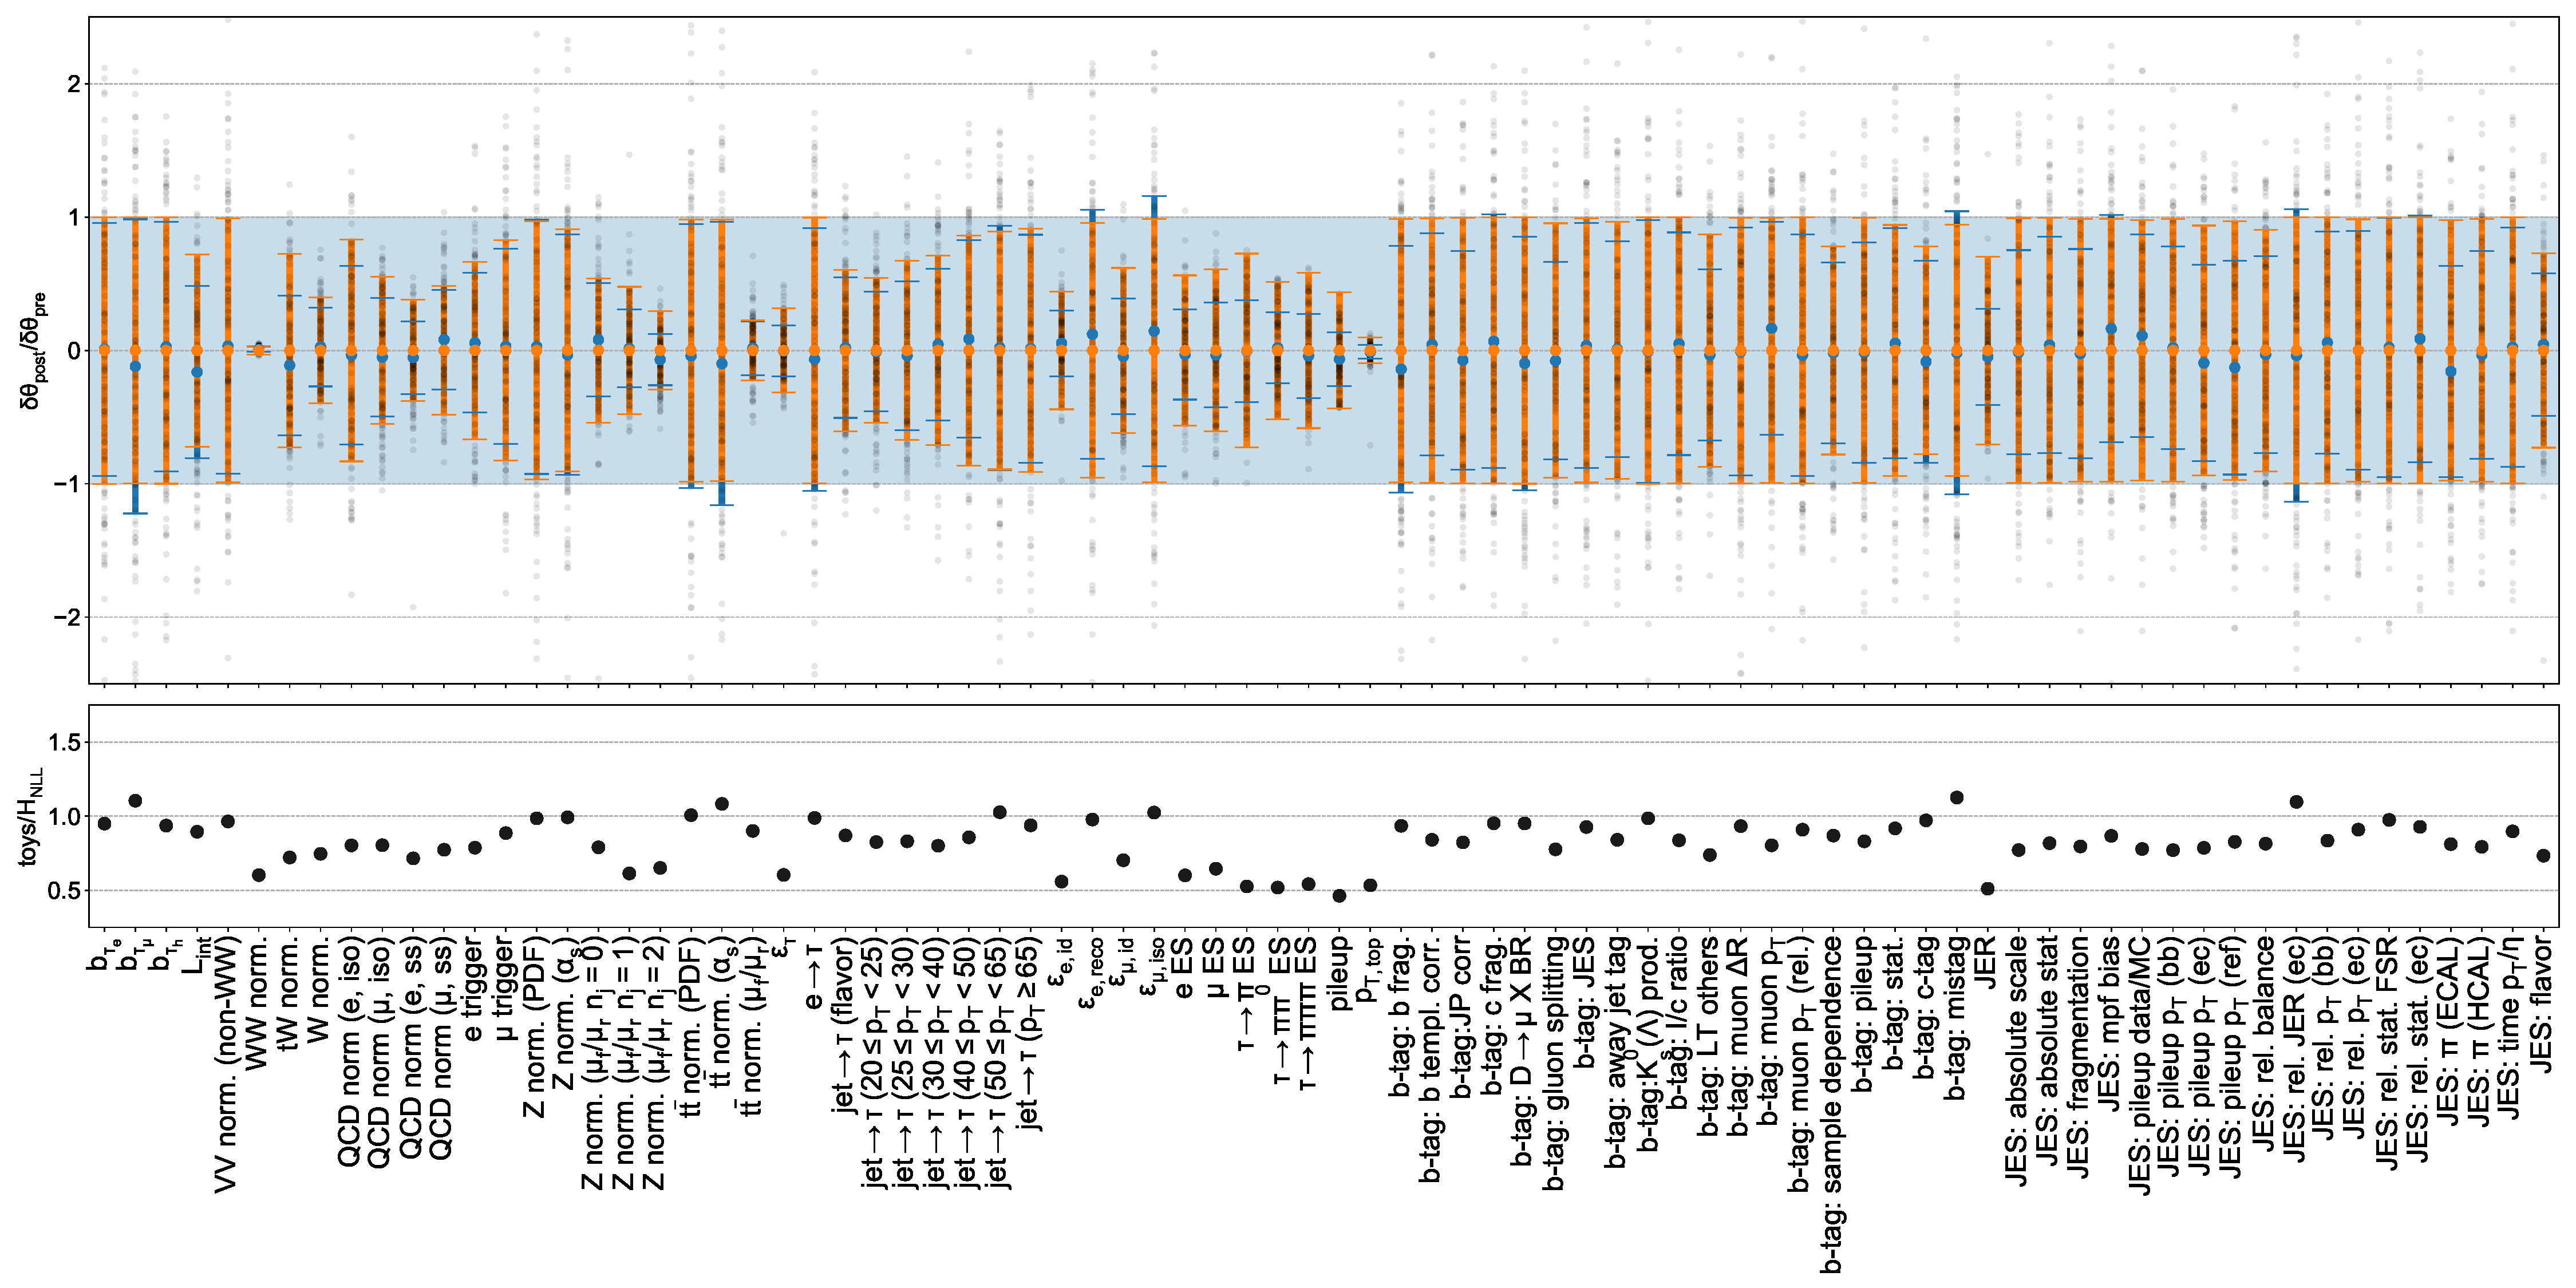
\includegraphics[width=0.9\textheight, angle=-90]{chapters/Analysis/sectionStatisticalAnalysis/figures/new_pulls}
    \caption{Pulls for nuisance parameters based on toy data while
        scanning the W boson leptonic branching fractions.  The black
        dots indicate the values for individual trials, the blue bars
        show the standard error estimated from those trials, and the
        orange bar are the values estimated from the Hessian of the NLL.}
    \label{fig:pulls_comparison}
\end{figure}




\subsubsection{Profile likelihood scans}

The covariance matrix associated with the likelihood is estimated using
numerical differentiation tools~\cite{numdifftools}.  In addition to
this, the variance associated with each parameter can be estimated by
scanning over values of the parameter near its minimum and minimizing
the likelihood while holding the parameter's value fixed.  The resulting
values of the NLL can then be fitted with a parabola to get the
associated standard error.  Because the full likelihood is just a sum of
the Poisson likelihoods for each bin, the likelihood associated with
each bin can also be studied.  This is useful for analyzing which
categories and which parts of the kinematical space are more sensitive
to different fit parameters.  

The result of scanning over the three leptonic branching fractions is
shown in figure~\ref{fig:beta_scan_1D}.  Curvatures of the NLL in each bin
of the analysis are estimated in the same way and presented in
figures~\ref{fig:ele_scan_bins}, \ref{fig:mu_scan_bins}, \ref{fig:tau_scan_bins}.
The figure shows the estimated curvature (variance) in each bin
normalized to the total variance.  The simplest way to interpret what is
shown is that a larger bar corresponds to a more significant
contribution to the sensitivity to the parameter under consideration.

\begin{figure}[h]
    \centering
    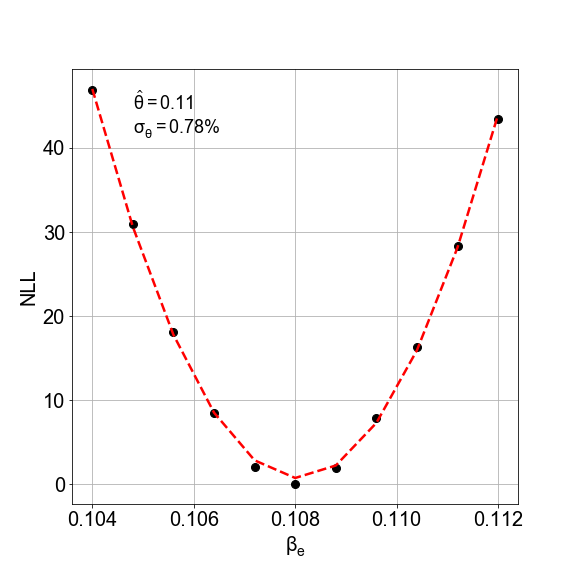
\includegraphics[width=0.32\textwidth]{chapters/Analysis/sectionStatisticalAnalysis/figures/beta_e}
    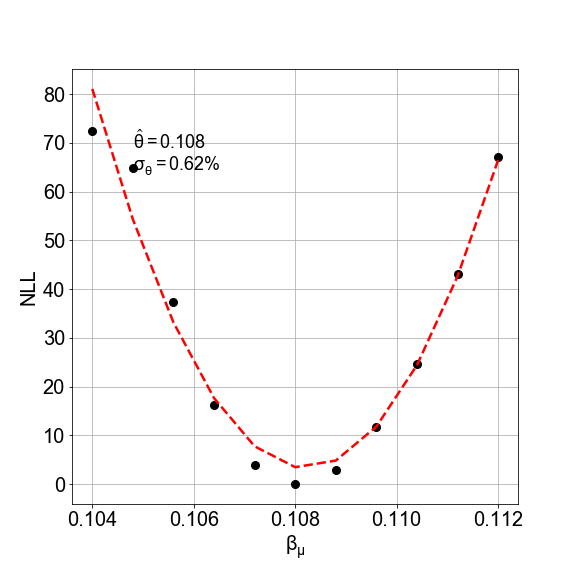
\includegraphics[width=0.32\textwidth]{chapters/Analysis/sectionStatisticalAnalysis/figures/beta_mu}
    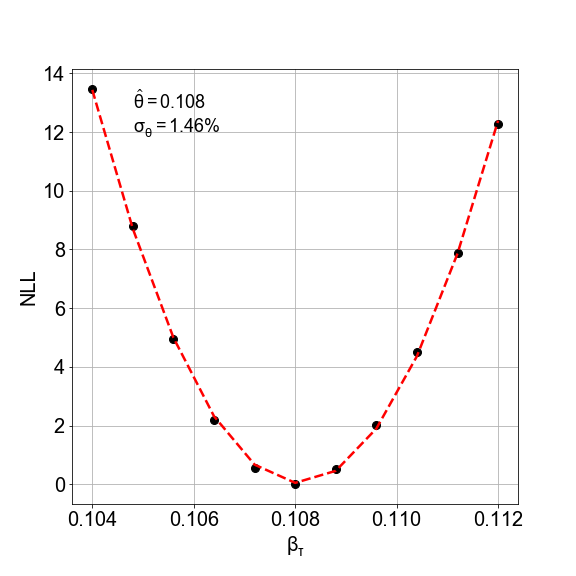
\includegraphics[width=0.32\textwidth]{chapters/Analysis/sectionStatisticalAnalysis/figures/beta_tau}
    \caption{Values for the NLL while scanning over the leptonic
    branching fractions of the \PW.}
    \label{fig:beta_scan_1D}
\end{figure}

\begin{figure}[htb!]
    \centering
    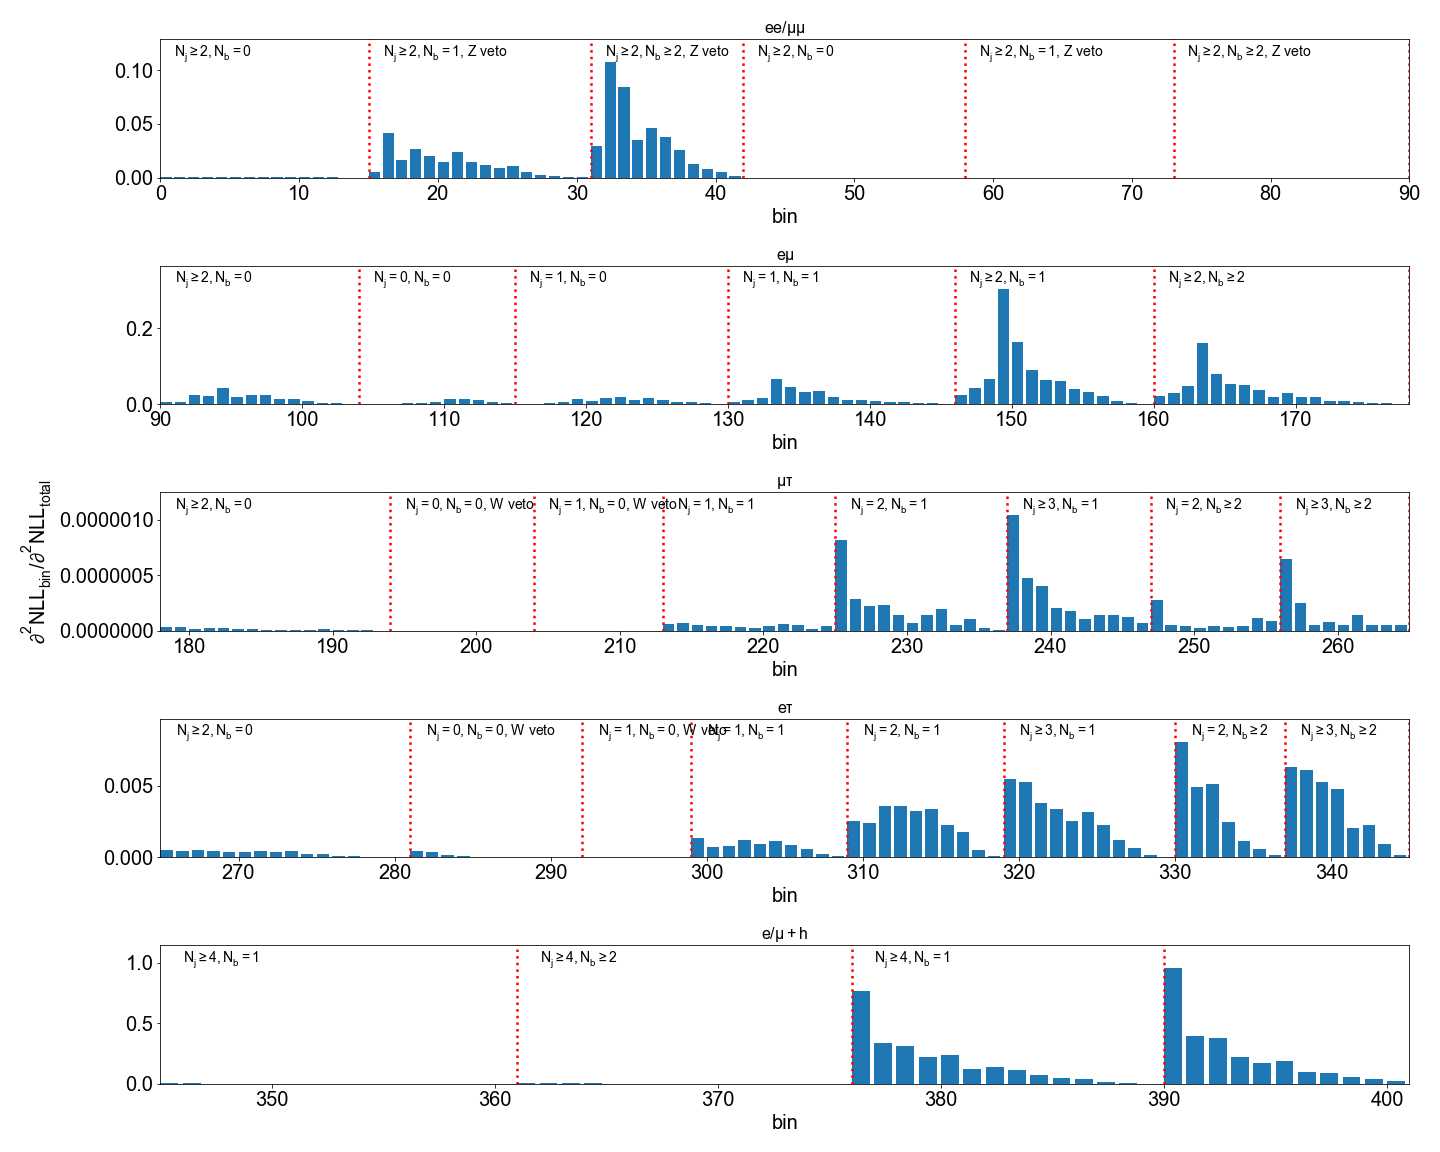
\includegraphics[width=\textwidth]{chapters/Analysis/sectionStatisticalAnalysis/figures/beta_e_scan_bins_lh}
    \caption{Bin-by-bin sensitivity for the electronic branching fraction. }
    \label{fig:ele_scan_bins}
\end{figure}

\begin{figure}[htb!]
    \centering
    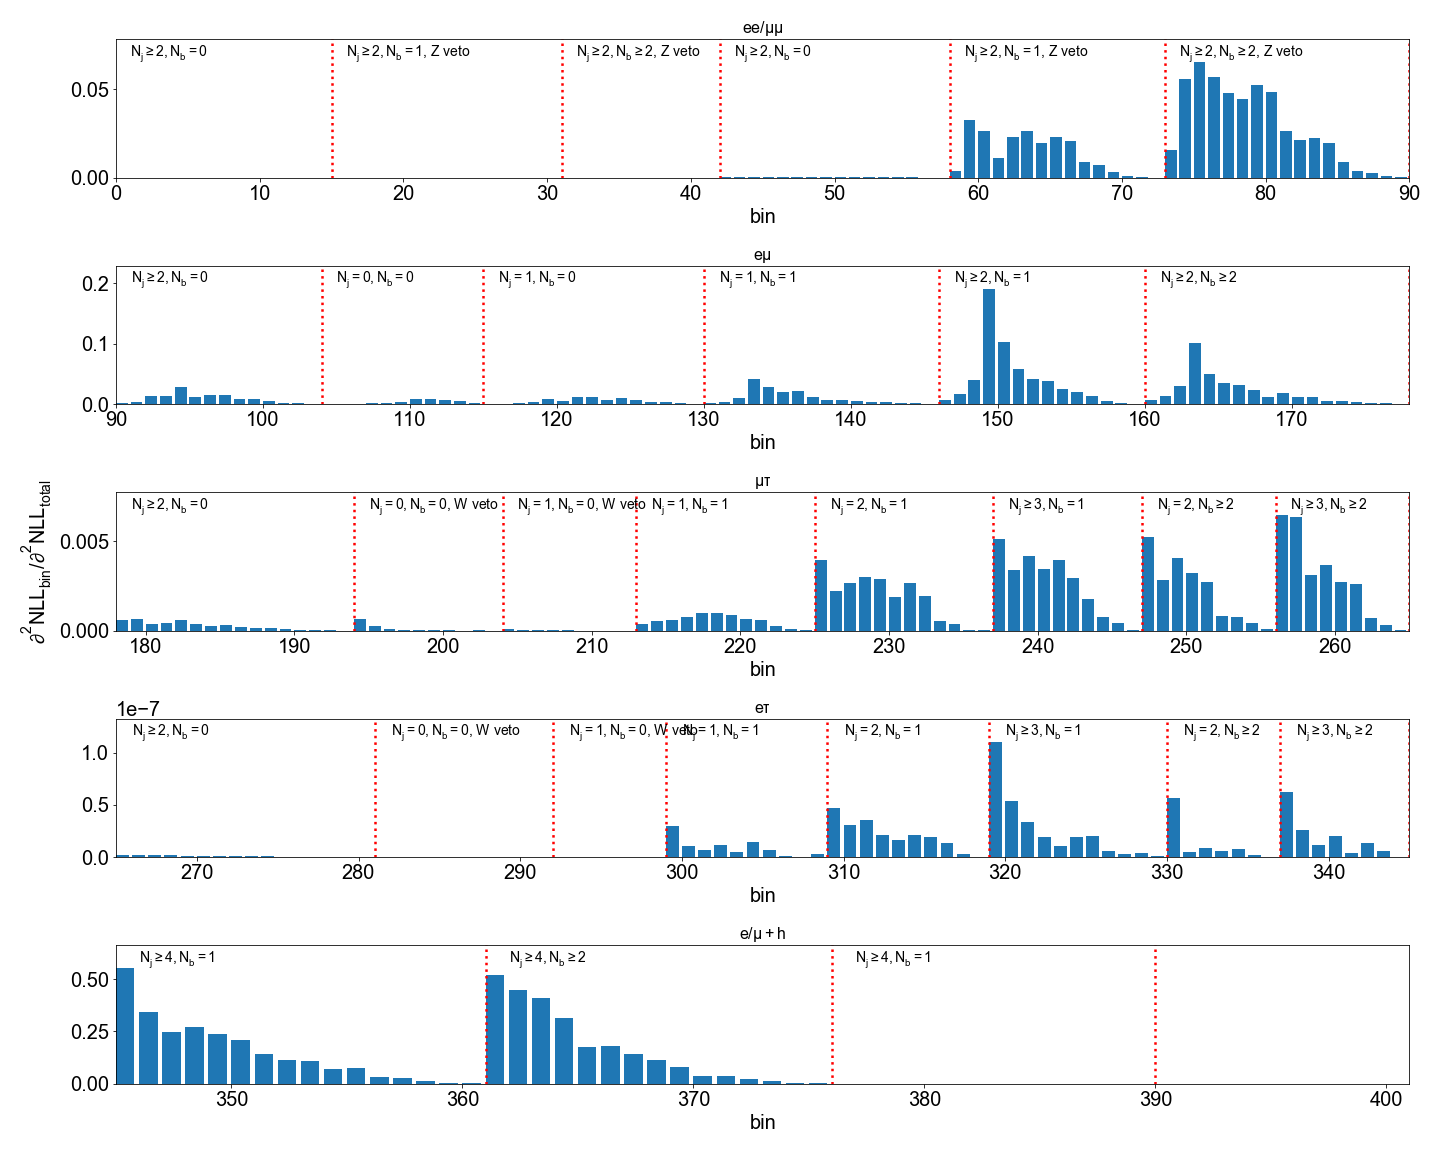
\includegraphics[width=\textwidth]{chapters/Analysis/sectionStatisticalAnalysis/figures/beta_mu_scan_bins_lh}
    \caption{Bin-by-bin sensitivity for the muonic branching fraction.}
    \label{fig:mu_scan_bins}
\end{figure}

\begin{figure}[htb!]
    \centering
    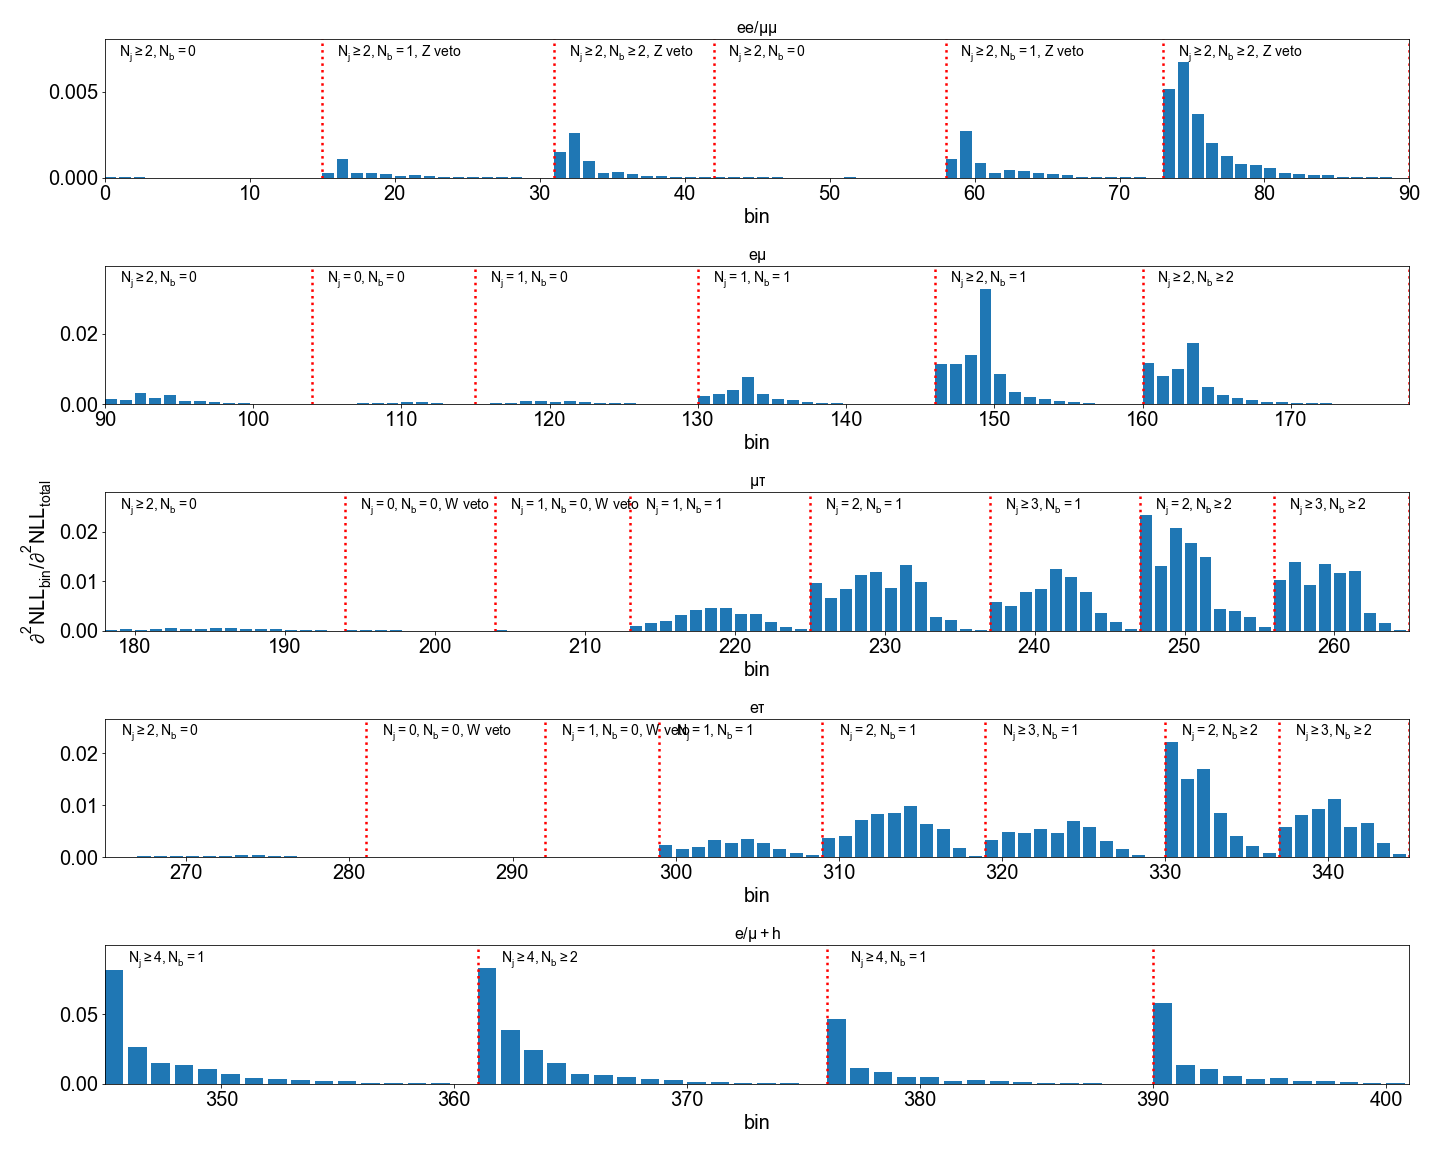
\includegraphics[width=\textwidth]{chapters/Analysis/sectionStatisticalAnalysis/figures/beta_tau_scan_bins_lh}
    \caption{Bin-by-bin sensitivity for the tauonic branching fraction.}
    \label{fig:tau_scan_bins}
\end{figure}


\FloatBarrier




%%%%%%%%%%%%%%%%%%%%%%%%%%%%%%%%%%%%%%%%
% 3. Counting Analysis
%%%%%%%%%%%%%%%%%%%%%%%%%%%%%%%%%%%%%%%%
\subsection{Counting Analysis}


\begin{figure}[htb!]
    \centering
    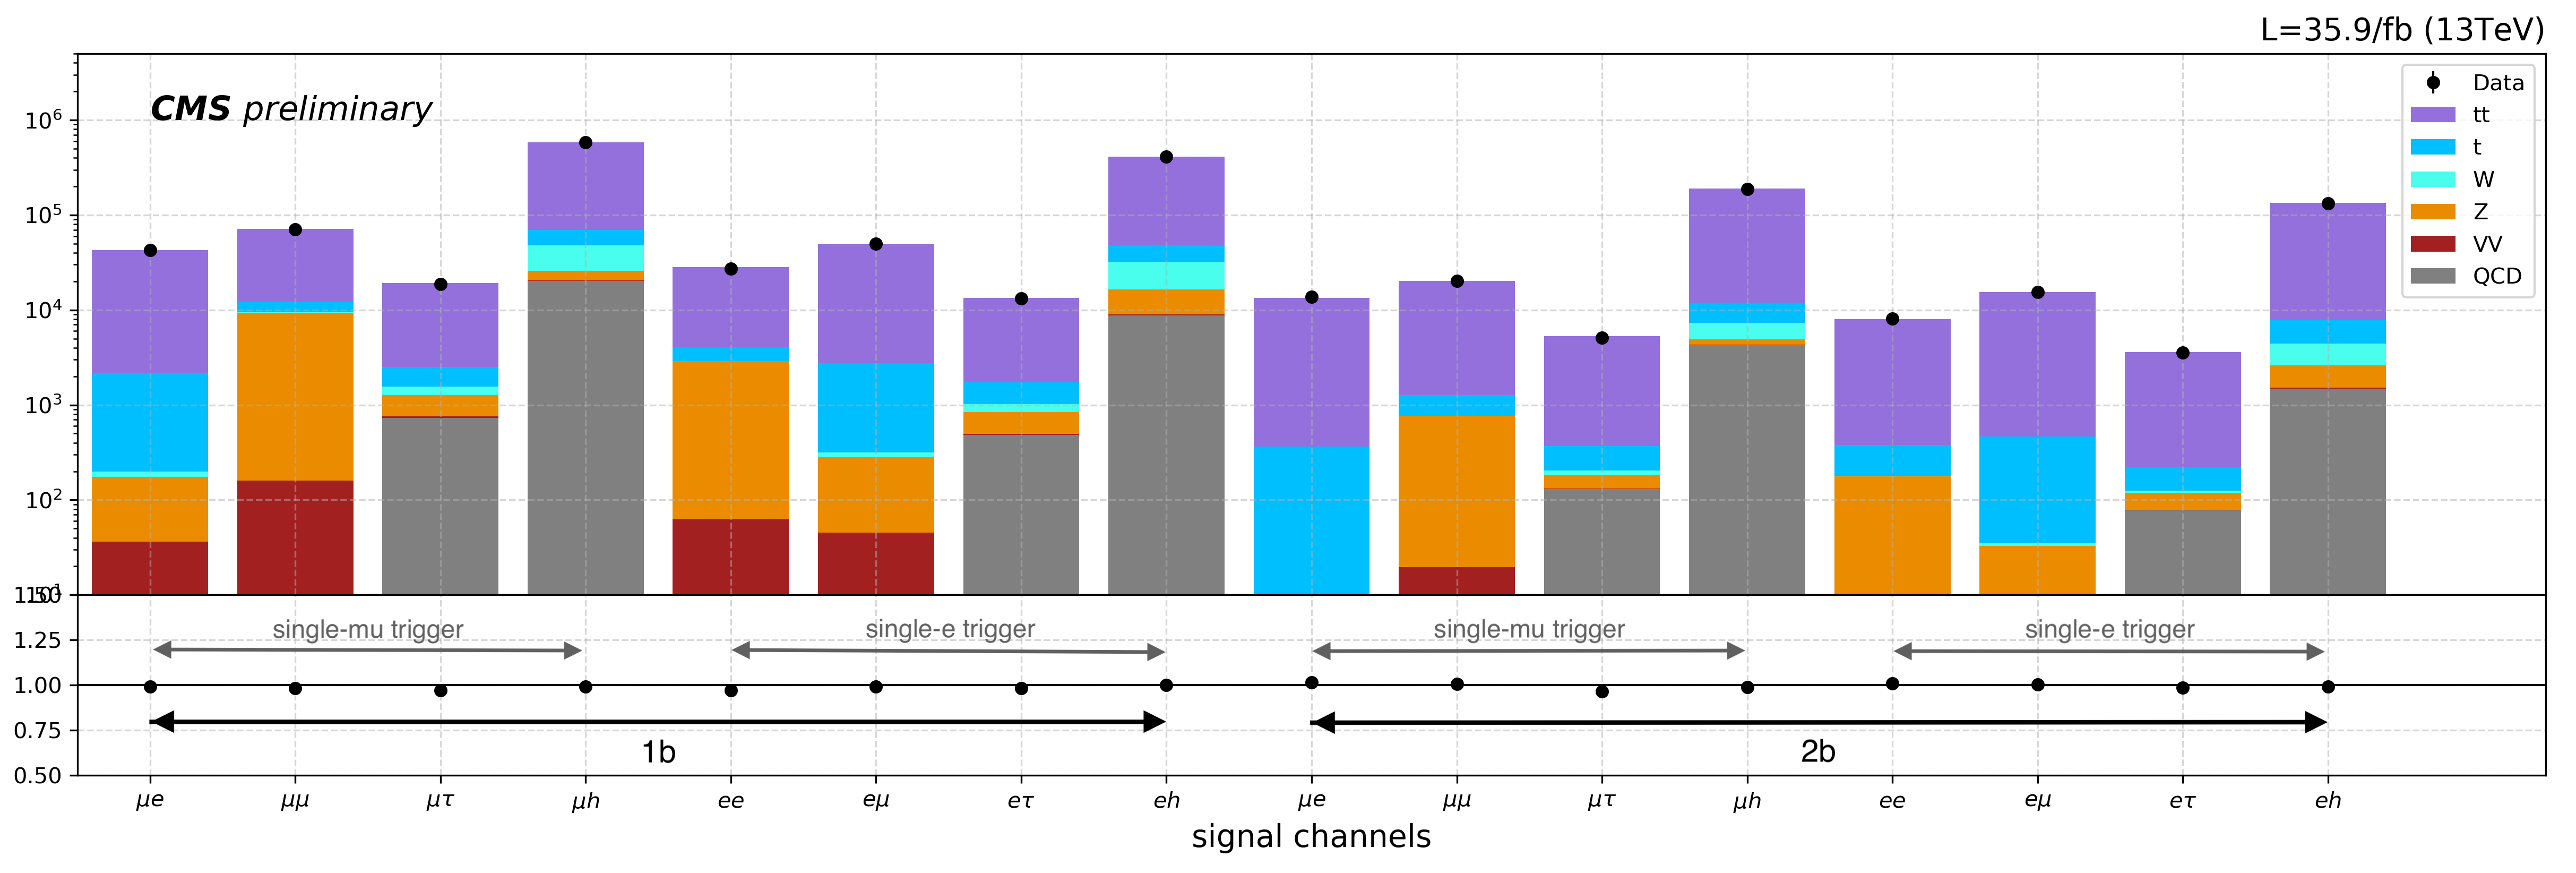
\includegraphics[width=0.99\textwidth]{chapters/Analysis/sectionStatisticalAnalysis/figures/counting.png}
    \caption{ Channels are organized into four groups based on trigger type and 
    b-tag multiplicity. Counting analysis extracts W branching fraction from the yields
    of grouped channels.}
    \label{fig:groupsofchannel}
\end{figure}

In this approach, channels are divided into four mutually-exclusive groups based on the trigger types and the b-tag multiplicities. 
The trigger types include the single-muon and the single-electron trigger. The b-tag multiplicity could be either $n_b=1$ or $n_b \geq 2$.
The configuration of four channel groups is shown in figure~\ref{fig:groupsofchannel}. Namely,

\begin{itemize}
    \item single-$\mu$ trigger with $n_b=1$ or $n_b \geq 2$ : $\big \{ \mu e, \mu\mu, \mu\tau, \mu h \big  \}$.
    \item single-$e$ trigger with $n_b=1$ or $n_b \geq 2$ : $ \big  \{ e e, e\mu, e\tau, e h \big  \}$ .
\end{itemize}


\noindent where $e\mu$ and $\mu e$ are mutually exclusive -- $e\mu$ channel
requires e-trigger with $p^T_e > p^T_\mu$, while $\mu e$ channel
requires $\mu$-trigger with $p^T_e < p^T_\mu$. 




To reject more $j\to \tau$ and QCD fakes, in the counting analysis, the thresholds of leptons' \pt 
and working point for the hadronic tau isolation are slightly tighten. 
This results in slightly different signal
acceptances comparing with the shape analysis. For the 8 channels under consideration, 
the signal efficiencies determined from
simulated \ttbar and tW events are shown in
tables \ref{tab:sigacc} and figure~\ref{fig:efficencyMatrix}. 

%In each of 16 channels, the signal constituents break down to 21 decay
%final states is shown in percentage in Table \ref{sigcomp}.


\begin{figure}[ht]
    \centering
    channels with $\mu$-trigger-1b \\
    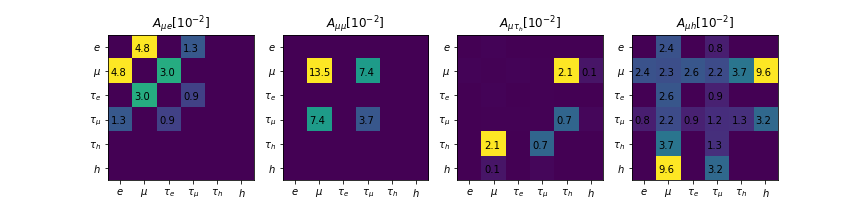
\includegraphics[width=\textwidth]{chapters/Analysis/sectionStatisticalAnalysis/figures/acc_mu1b.png}
    
    channels with $\mu$-trigger-2b \\
    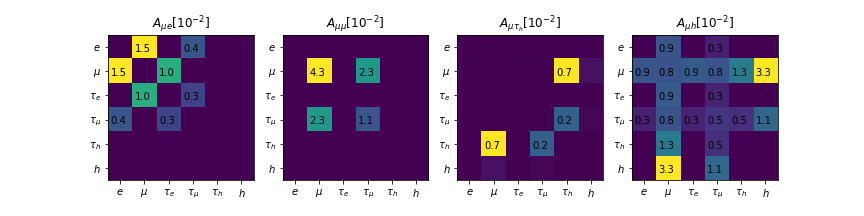
\includegraphics[width=\textwidth]{chapters/Analysis/sectionStatisticalAnalysis/figures/acc_mu2b.png}
    
    channels with $e$-trigger-1b \\
    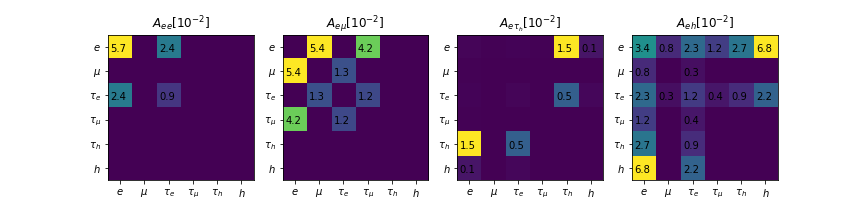
\includegraphics[width=\textwidth]{chapters/Analysis/sectionStatisticalAnalysis/figures/acc_e1b.png}
    
    channels with $e$-trigger-2b \\
    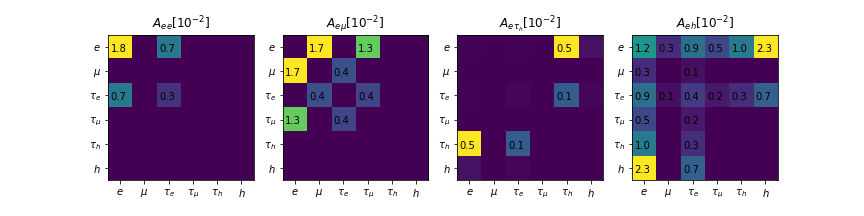
\includegraphics[width=\textwidth]{chapters/Analysis/sectionStatisticalAnalysis/figures/acc_e2b.png}
    
    %--------------------------
    \caption{ Efficiency matrices \textbf{E} of four groups based on trigger types and the b-tag multiplicities. }
    \label{fig:efficencyMatrix}
\end{figure}





\begin{sidewaystable}[p]
    \centering
    \setlength{\tabcolsep}{0.4em}
    \renewcommand{\arraystretch}{1.5}
    \caption{Efficiency of $t\bar{t}$+$tW$ events, breakdown by 21 WW decay.  Values are in percent.}
    
    \resizebox{\textwidth}{!}{
    \begin{tabular}{|l|cc|cc|cc|cc|cc|cc|cc|cc|}
    
    
    \hline
    channel & \multicolumn{2}{|c|}{$\mu e$} & \multicolumn{2}{c|}{$\mu\mu$} & \multicolumn{2}{|c|}{$\mu \tau$} & \multicolumn{2}{|c|}{$\mu$+jets} & \multicolumn{2}{|c|}{$ee$} & \multicolumn{2}{|c|}{$e\mu$} & \multicolumn{2}{|c|}{$e \tau$} & \multicolumn{2}{|c|}{$e+jets$} \\
    \hline
    $\rm n_{b tag}$ & $n_b=1$ & $n_b\geq2$ & $n_b=1$ & $n_b\geq2$ & $n_b=1$ & $n_b\geq2$ & $n_b=1$ & $n_b\geq2$ & $n_b=1$ & $n_b\geq2$ & $n_b=1$ & $n_b\geq2$ & $n_b=1$ & $n_b\geq2$ & $n_b=1$ & $n_b\geq2$ \\ 
    \hline
    
    $tt/tW \to ee$                     &    --    &    --    &    --    &    --    &    --    &    --    &    --    &    --    &  5.71(1) &  3.19(1) &    --    &    --    &    --    &    --    &  3.17(1) &  2.14(1) \\ 
    $tt/tW \to \mu\mu$                 &    --    &    --    & 14.14(2) &  8.02(1) &    --    &    --    &  1.80(1) &  1.21(0) &    --    &    --    &    --    &    --    &    --    &    --    &    --    &    --    \\ 
    $tt/tW \to e\mu$                   &  4.69(1) &  2.66(0) &    --    &    --    &    --    &    --    &  2.35(0) &  1.60(0) &    --    &    --    &  5.76(1) &  3.24(1) &    --    &    --    &  0.71(0) &  0.48(0) \\ 
    $tt/tW \to \tau_{e}\tau_{e}$       &    --    &    --    &    --    &    --    &    --    &    --    &    --    &    --    &  0.74(2) &  0.44(2) &    --    &    --    &    --    &    --    &  1.18(4) &  0.81(2) \\ 
    $tt/tW \to \tau_{\mu}\tau_{\mu}$   &    --    &    --    &  3.88(5) &  2.11(4) &    --    &    --    &  1.13(3) &  0.77(2) &    --    &    --    &    --    &    --    &    --    &    --    &    --    &    --    \\ 
    $tt/tW \to \tau_{e}\tau_{\mu}$     &  0.78(2) &  0.45(1) &    --    &    --    &    --    &    --    &  0.92(2) &  0.62(1) &    --    &    --    &  1.24(2) &  0.70(2) &    --    &    --    &  0.40(1) &  0.27(1) \\ 
    $tt/tW \to \tau_{e}\tau_{h}$       &    --    &    --    &    --    &    --    &    --    &    --    &    --    &    --    &    --    &    --    &    --    &    --    &  0.48(1) &  0.26(0) &  0.84(1) &  0.61(1) \\ 
    $tt/tW \to \tau_{\mu}\tau_{h}$     &    --    &    --    &    --    &    --    &  0.74(1) &  0.40(1) &  1.28(1) &  0.92(1) &    --    &    --    &    --    &    --    &    --    &    --    &    --    &    --    \\ 
    $tt/tW \to \tau_{h}\tau_{h}$       &    --    &    --    &    --    &    --    &    --    &    --    &    --    &    --    &    --    &    --    &    --    &    --    &    --    &    --    &    --    &    --    \\ 
    $tt/tW \to e\tau_{e}$              &    --    &    --    &    --    &    --    &    --    &    --    &    --    &    --    &  2.14(1) &  1.18(1) &    --    &    --    &    --    &    --    &  2.29(1) &  1.62(1) \\ 
    $tt/tW \to e\tau_{\mu}$            &  1.28(1) &  0.69(1) &    --    &    --    &    --    &    --    &  0.80(1) &  0.54(0) &    --    &    --    &  4.49(2) &  2.47(1) &    --    &    --    &  1.18(1) &  0.86(1) \\ 
    $tt/tW \to e\tau_{h}$              &    --    &    --    &    --    &    --    &    --    &    --    &    --    &    --    &    --    &    --    &    --    &    --    &  1.59(1) &  0.88(0) &  2.61(1) &  1.90(0) \\ 
    $tt/tW \to \mu\tau_{e}$            &  2.54(1) &  1.43(1) &    --    &    --    &    --    &    --    &  2.61(1) &  1.86(1) &    --    &    --    &  1.42(1) &  0.78(1) &    --    &    --    &  0.23(0) &  0.16(0) \\ 
    $tt/tW \to \mu\tau_{\mu}$          &    --    &    --    &  7.76(2) &  4.37(2) &    --    &    --    &  1.88(1) &  1.35(1) &    --    &    --    &    --    &    --    &    --    &    --    &    --    &    --    \\ 
    $tt/tW \to \mu\tau_{h}$            &    --    &    --    &    --    &    --    &  2.27(1) &  1.27(0) &  3.70(1) &  2.70(1) &    --    &    --    &    --    &    --    &    --    &    --    &    --    &    --    \\ 
    $tt/tW \to eh$                     &    --    &    --    &    --    &    --    &    --    &    --    &    --    &    --    &    --    &    --    &    --    &    --    &  0.10(0) &    --    &  6.83(0) &  4.64(0) \\ 
    $tt/tW \to \mu h$                  &    --    &    --    &    --    &    --    &  0.15(0) &    --    &  9.71(1) &  6.61(0) &    --    &    --    &    --    &    --    &    --    &    --    &    --    &    --    \\ 
    $tt/tW \to \tau_{e}h$              &    --    &    --    &    --    &    --    &    --    &    --    &    --    &    --    &    --    &    --    &    --    &    --    &    --    &    --    &  2.17(1) &  1.44(0) \\ 
    $tt/tW \to \tau_{\mu}h$            &    --    &    --    &    --    &    --    &    --    &    --    &  3.30(1) &  2.19(1) &    --    &    --    &    --    &    --    &    --    &    --    &    --    &    --    \\ 
    $tt/tW \to \tau_{h}h$              &    --    &    --    &    --    &    --    &    --    &    --    &    --    &    --    &    --    &    --    &    --    &    --    &    --    &    --    &    --    &    --    \\ 
    $tt/tW \to hh$                     &    --    &    --    &    --    &    --    &    --    &    --    &    --    &    --    &    --    &    --    &    --    &    --    &    --    &    --    &    --    &    --    \\ 

    \hline
    \end{tabular}}
    
    \label{tab:sigacc}
    
\end{sidewaystable}





\subsubsection{Parameter Extraction}


In each of the channel groups above, three branching fractions $\beta_e,\beta_\mu,\beta_\tau$ are extracted by solving a set of
three quadratic equations. Then the results from all four groups are combined taking into account 
the uncorrelated statistical uncertainties and full-correlated systematical uncertainties. The details of the
combine is described in Section~\ref{sec:analysis:systematics}. Here gives the method of parameter extraction
by establishing and solving quadratic equations.


The normalized yield $X$, which is constructed in a similar manner to the branching fractions, 
is the ratio of yield in one channel over the sum of yields in the channel group. 
For channel group using single-electron and single-muon trigger, 
denoting the triggering lepton as $t\in \{\mu,e\}$, 
the normalized yields $X$'s are defined as
\begin{equation}
    X_{e}   = \frac{n^{t e}     }{n^{t e} + n^{t \mu} + n^{t \tau} + n^{t h}},
    X_{\mu} = \frac{n^{t \mu}   }{n^{t e} + n^{t \mu} + n^{t \tau} + n^{t h}}, 
    X_{\tau}= \frac{n^{t \tau}  }{n^{t e} + n^{t \mu} + n^{t \tau} + n^{t h}},
\end{equation}

\noindent where $n \equiv N - \sum_{b} N_b $ is the data yield with background subtracted. 
Based on Eqn \ref{eq:data_model}, the normalized yields $\{X_{e},X_{\mu},X_{\tau}\}$ from data should 
equal to the same calculation based on the efficiency \textbf{E} matrix and the branching fraction matrix \textbf{B}:
% 
\begin{equation} \label{quadEqA}
    \begin{split}
    X_e     &= \frac{ E_{ij}^{te}B_{ij}     }{  E_{ij}^{te}B_{ij} + E_{ij}^{t\mu}B_{ij} + E_{ij}^{t\tau}B_{ij} + E_{ij}^{th}B_{ij}} ,\\
    X_\mu   &= \frac{ E_{ij}^{t\mu}B_{ij}   }{  E_{ij}^{te}B_{ij} + E_{ij}^{t\mu}B_{ij} + E_{ij}^{t\tau}B_{ij} + E_{ij}^{th}B_{ij}} ,\\
    X_\tau  &= \frac{ E_{ij}^{t\tau}B_{ij}  }{  E_{ij}^{te}B_{ij} + E_{ij}^{t\mu}B_{ij} + E_{ij}^{t\tau}B_{ij} + E_{ij}^{th}B_{ij}}.
    \end{split}
\end{equation}


\noindent Plugging in the explicit form of \textbf{E} and \textbf{B} matrices in Eqn \ref{eq:br_matrix} 
and Eqn \ref{eq:eff_matrix} and the unity condition $\beta_h = 1- \beta_e -
\beta_\mu - \beta_\tau$, Eqn \ref{quadEqA} can be written as a set of
three quadratic equations with three unknowns $\{\beta_{e},\beta_{\mu},\beta_{\tau}\}$.
% 
\begin{singlespace}
\begin{equation} \label{quadEqB}
    \small
	\begin{split}
        c_{e1} \beta_e^2 + c_{e2} \beta_\mu^2 + c_{e3} \beta_\tau^2 + 
        c_{e4} \beta_e\beta_\mu + c_{e5} \beta_e\beta_\tau + c_{e6} \beta_\mu\beta_\tau +
        c_{e7} \beta_e + c_{e8} \beta_\mu + c_{e9} \beta_\tau + c_{e0} &\\
        = F_e(\beta_e,\beta_\mu,\beta_\tau) = 0 &,\\
        %
        c_{\mu 1} \beta_e^2 + c_{\mu 2} \beta_\mu^2 + c_{\mu 3} \beta_\tau^2 + 
        c_{\mu 4} \beta_e\beta_\mu + c_{\mu 5} \beta_e\beta_\tau + c_{\mu 6} \beta_\mu\beta_\tau +
        c_{\mu 7} \beta_e + c_{\mu 8} \beta_\mu + c_{\mu 9} \beta_\tau + c_{\mu 0} &\\
        = F_\mu(\beta_e,\beta_\mu,\beta_\tau) = 0 &, \\
        %
        c_{_\tau1} \beta_e^2 + c_{\tau2} \beta_\mu^2 + c_{\tau3} \beta_\tau^2 + 
        c_{\tau4} \beta_e\beta_\mu + c_{\tau5} \beta_e\beta_\tau + c_{\tau6} \beta_\mu\beta_\tau +
        c_{\tau7} \beta_e + c_{\tau8} \beta_\mu + c_{\tau9} \beta_\tau + c_{\tau0} &\\
        = F_\tau(\beta_e,\beta_\mu,\beta_\tau) = 0 &,
    \end{split}
\end{equation}
\end{singlespace}


\noindent where the coefficients $c_{lk}$, with the index $l\in \{ e,\mu,\tau \}$ corresponding
to the three equations $F_e=0,F_\mu=0,F_\tau=0$ and the index $k\in\{ 0,1,2,\dots 9\}$,
are fully determined by efficiency matrix \textbf{E} and normalized yields $\{X_e,X_\mu,X_\tau\}$.
The analytical result of $c_{lk}$ is listed in table~\ref{tab:quadcoeff}.

\begin{table}[ht]
    \centering
   	\setlength{\tabcolsep}{0.4em}
    \renewcommand{\arraystretch}{1.5}
    \small
    
    \begin{tabular}{c|l}

    \hline
    $c_{l0}$ & $\Delta_{hh}$ \\
    \hline
    $c_{l1}$ & $\Delta_{ee}     - 2\Delta_{eh}   + \Delta_{hh}$ \\
    \hline
    $c_{l2}$ & $\Delta_{\mu\mu} - 2\Delta_{\mu h} + \Delta_{hh}$ \\
    \hline
    
    $c_{l3}$ & $   b^\tau_e   b^\tau_e   \Delta_{\tau_e   \tau_e}  
    			 + b^\tau_\mu b^\tau_\mu \Delta_{\tau_\mu \tau_\mu}
                 + b^\tau_h   b^\tau_h   \Delta_{\tau_h   \tau_h}
                 
                 + 2 b^\tau_e   b^\tau_\mu \Delta_{\tau_e   \tau_\mu} 
    		     + 2 b^\tau_e   b^\tau_h   \Delta_{\tau_e   \tau_h}   
    		     + 2 b^\tau_\mu b^\tau_h   \Delta_{\tau_\mu \tau_h} - $ \\
                 
             & $   2 b^\tau_e   \Delta_{e   \tau_h}
                 - 2 b^\tau_\mu \Delta_{\mu \tau_h}
                 - 2 b^\tau_h   \Delta_{h.  \tau_h} 
                 + \Delta_{hh} $ \\

    \hline
    $c_{l4}$ & $2\Delta_{e\mu} - 2\Delta_{eh} -2\Delta_{\mu h} +2\Delta_{hh}$  \\
    \hline
    $c_{l5}$ & $  2b^\tau_e   \Delta_{e \tau_e} 
    			+ 2b^\tau_\mu \Delta_{e \tau_\mu}
                + 2b^\tau_h   \Delta_{e \tau_h}
                - 2b^\tau_e   \Delta_{\tau_e   h} 
    			- 2b^\tau_\mu \Delta_{\tau_\mu h}
                - 2b^\tau_h   \Delta_{\tau_h   h} 
                - 2\Delta_{eh}   + 2 \Delta_{hh} $ \\
        
    \hline            
    $c_{l6}$ & $  2b^\tau_e   \Delta_{\mu \tau_e} 
    			+ 2b^\tau_\mu \Delta_{\mu \tau_\mu}
                + 2b^\tau_h   \Delta_{\mu \tau_h}
                - 2b^\tau_e   \Delta_{\tau_e   h} 
    			- 2b^\tau_\mu \Delta_{\tau_\mu h}
                - 2b^\tau_h   \Delta_{\tau_h   h} 
                - 2\Delta_{\mu h}   + 2 \Delta_{hh} $ \\
    \hline            
    $c_{l7}$ & $ 2\Delta_{eh}      - 2 \Delta_{hh} $ \\
    \hline
    $c_{l8}$ & $ 2\Delta_{\mu h}   - 2 \Delta_{hh}$ \\
    \hline
    $c_{l9}$ & $  2b^\tau_e   \Delta_{\tau_e   h} 
                 + 2b^\tau_\mu \Delta_{\tau_\mu h} 
                 + 2b^\tau_h   \Delta_{\tau_h   h} 
                 - 2 \Delta_{hh}$ \\
    \hline
    \hline
    where  & $ \Delta \equiv E^{tl} - X_l \times ( E^{te} + E^{t\mu} + E^{t\tau} + E^{th} )$ \\
           & $l=e,\mu,\tau$ and $t=e(\mu)$ if using single-$e$ (signle-$\mu$) trigger\\
    \hline
    
	\end{tabular}
    
\caption{ Coefficients of quadratic equations in terms of E and X. In the table, $l=e,\mu,\tau$ and $t=\mu,e$ for single-$\mu$ and single-$e$ trigger respectively.  }
\label{quadcoeff}
    
\end{table}

\begin{figure}[ht]
    \centering
    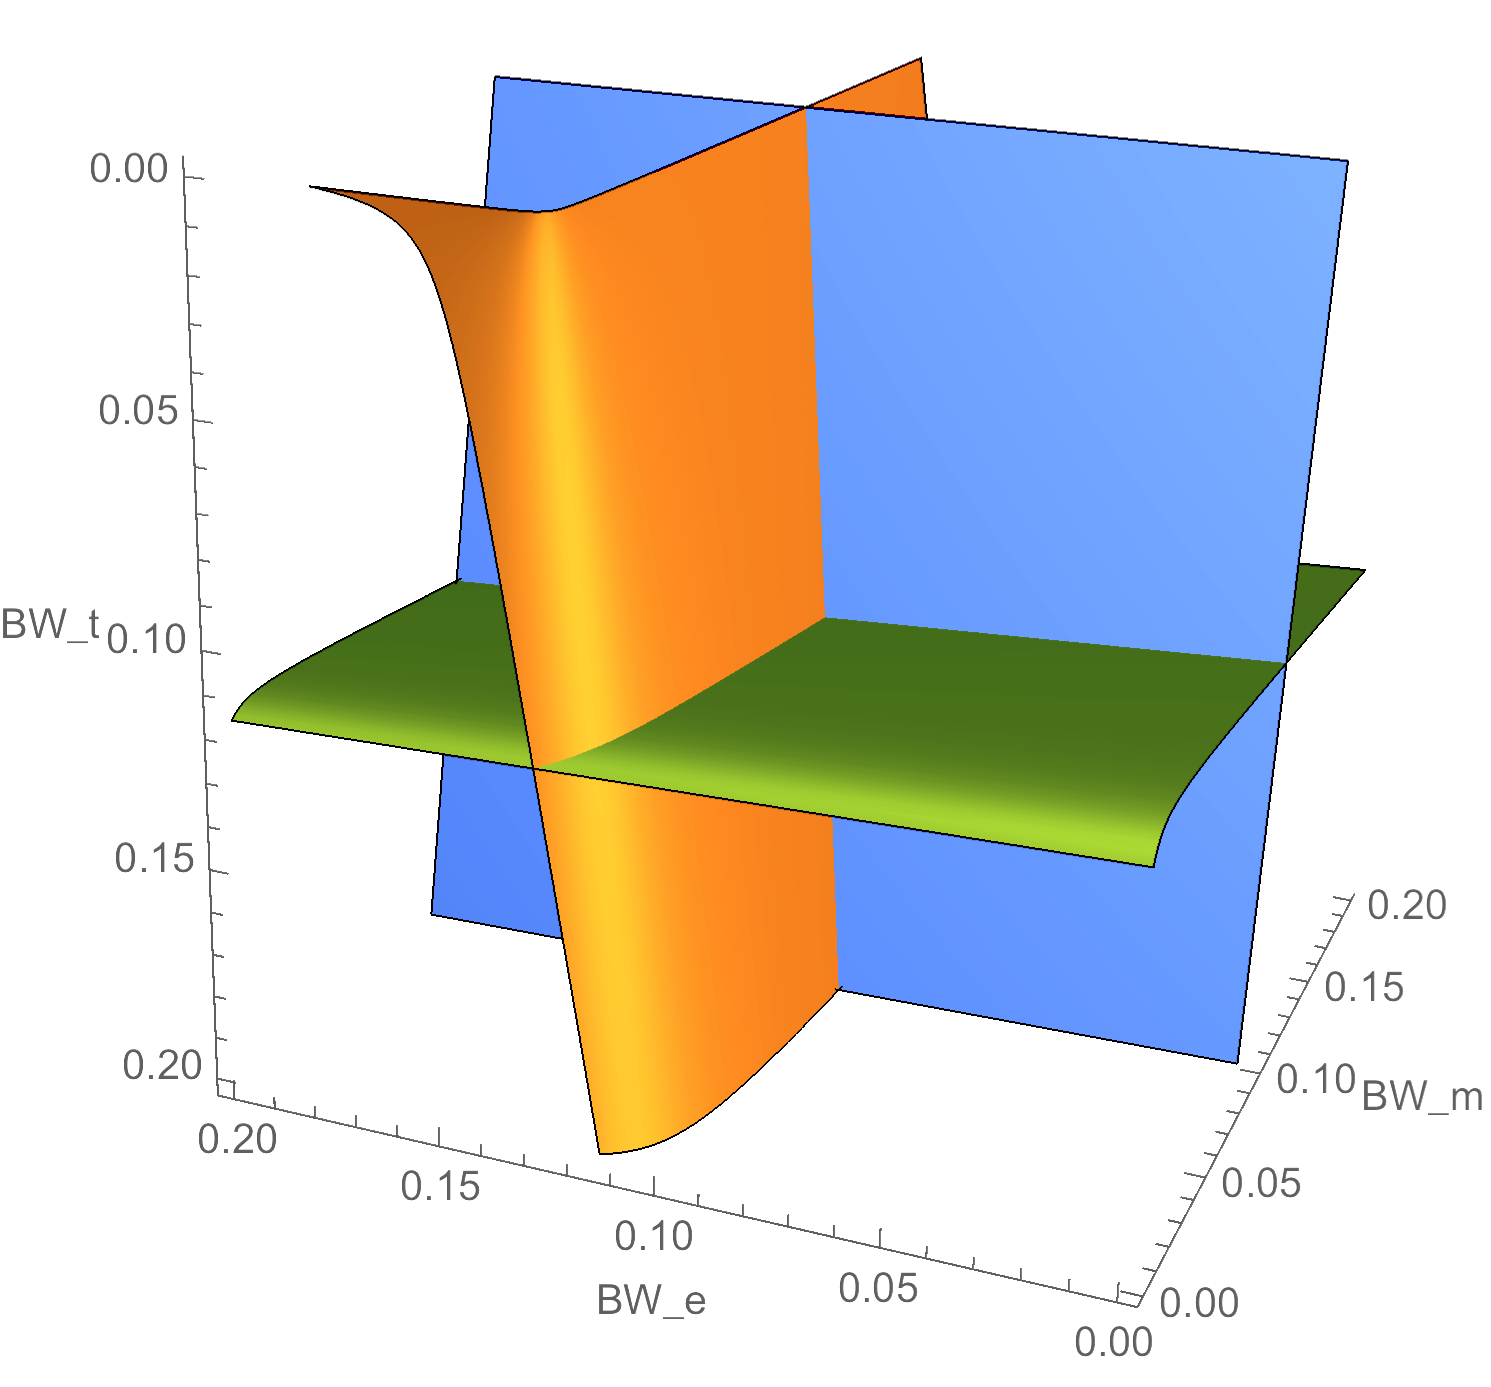
\includegraphics[width=7cm]{chapters/Analysis/sectionStatisticalAnalysis/figures/visual.png}
    \caption{ Visualization of Eq \ref{quadEqB} in the
    $\{\beta_{e},\beta_{\mu},\beta_{\tau}\}$ parameter space. Each
    equation in Eq \ref{quadEqB} is a hyperbolic plane, while their
    intersection is the solution Eq \ref{quadEqB}. Mathematically, there
    are 8 possible solutions. However, only one solution is physical,
    located with $\beta \in (0,1) $. }
    \label{fig:visualize}
\end{figure}


In the $\{\beta_{e},\beta_{\mu},\beta_{\tau}\}$ parameter space, 
equations in Eqn~\ref{quadEqB} represent three hyperbolic planes.
Figure~\ref{fig:visualize} shows a visualization of the three hyperbolic planes 
in the $\{\beta_{e},\beta_{\mu},\beta_{\tau}\}$ parameter space. 
The intersection of the three planes is the solution to the three equations, 
the targeted branching fractions to extract. Namely,
% 
\begin{equation} 
    \begin{bmatrix} 
        \beta_e \\ 
        \beta_\mu \\ 
        \beta_\tau 
    \end{bmatrix}
    = \text{Solution}
    \begin{bmatrix}
	    F_e    (\beta_e,\beta_\mu,\beta_\tau) = 0 \\
	    F_\mu  (\beta_e,\beta_\mu,\beta_\tau) = 0 \\
	    F_\tau (\beta_e,\beta_\mu,\beta_\tau) = 0
    \end{bmatrix}
\end{equation}



\subsubsection{Assessment of statistical uncertainties}
The statistical uncertainties of data in channels are propagated to the $\beta_l$ 
via the numerically calculated derivatives $\partial_{N} \beta_l$. 
The statistical uncertainties of yields in different channels are treated as uncorrelated, 
and are summed in quadrature after propagated to $\beta_l$.

The statistical uncertainties due to the background 
MC statistics are estimated by the same error propagation approach.
The statistical uncertainties of the signal MC are embedded in the statistical uncertainties 
of the \textbf{E} matrix based on equation~\ref{eq:model_eff}. The statistical uncertainty of 
efficiency is obtained by an integral of beta distribution, the conjugate of the
binomial distribution. The statistical uncertainties of \textbf{E} matrix are 
propagated to the $\beta_l$ the derivatives $\partial_{E_{ij}} \beta_l$, where the 
21 $E_{ij}$ elements are treated as uncorrelated and their impacts to $\beta_l$ are 
summed in quadrature. 


\subsubsection{Assessment of systematical uncertainties}

The systematical uncertainties are estimated by variating up and down the systematical parameters, and then
repeating the same process of parameter extraction. The corresponding deviations with respect to the nominal $\beta_l$
represent the systematical uncertainties. The $\Delta \beta_l$ due to the same systematical source in the four
channel groups are fully correlated. Different systematical sources are treated as independent. 
The total systematical uncertainty of $\beta_l$ combines the contributions from all independent systematical sources.


\subsubsection{Study of statistical bias of parameters}
A test of parameter extraction is performed using toy datasets.
In each toy dataset, the yield $N$ equals to the expected yield based MC with 
a statistical uncertainty of $\delta N = \sqrt{N}$. Then $\beta_l$ are 
extracted. In total, 2000 toys are generated. The W to lepton branching 
fractions in the MC are $10.8\%$, to which the extracted parameters are compared.
The distribution of $\{\beta_{e},\beta_{\mu},\beta_{\tau}\}$ extracted from the toys are shown in
figure~\ref{fig:test_toy}. The centers of distributions are consistent with
the assumed branching fraction in the MC, while widths of distributions are 
consistent with the data statistical uncertainty calculated by error propagation.





\begin{figure}[ht]
    \centering
    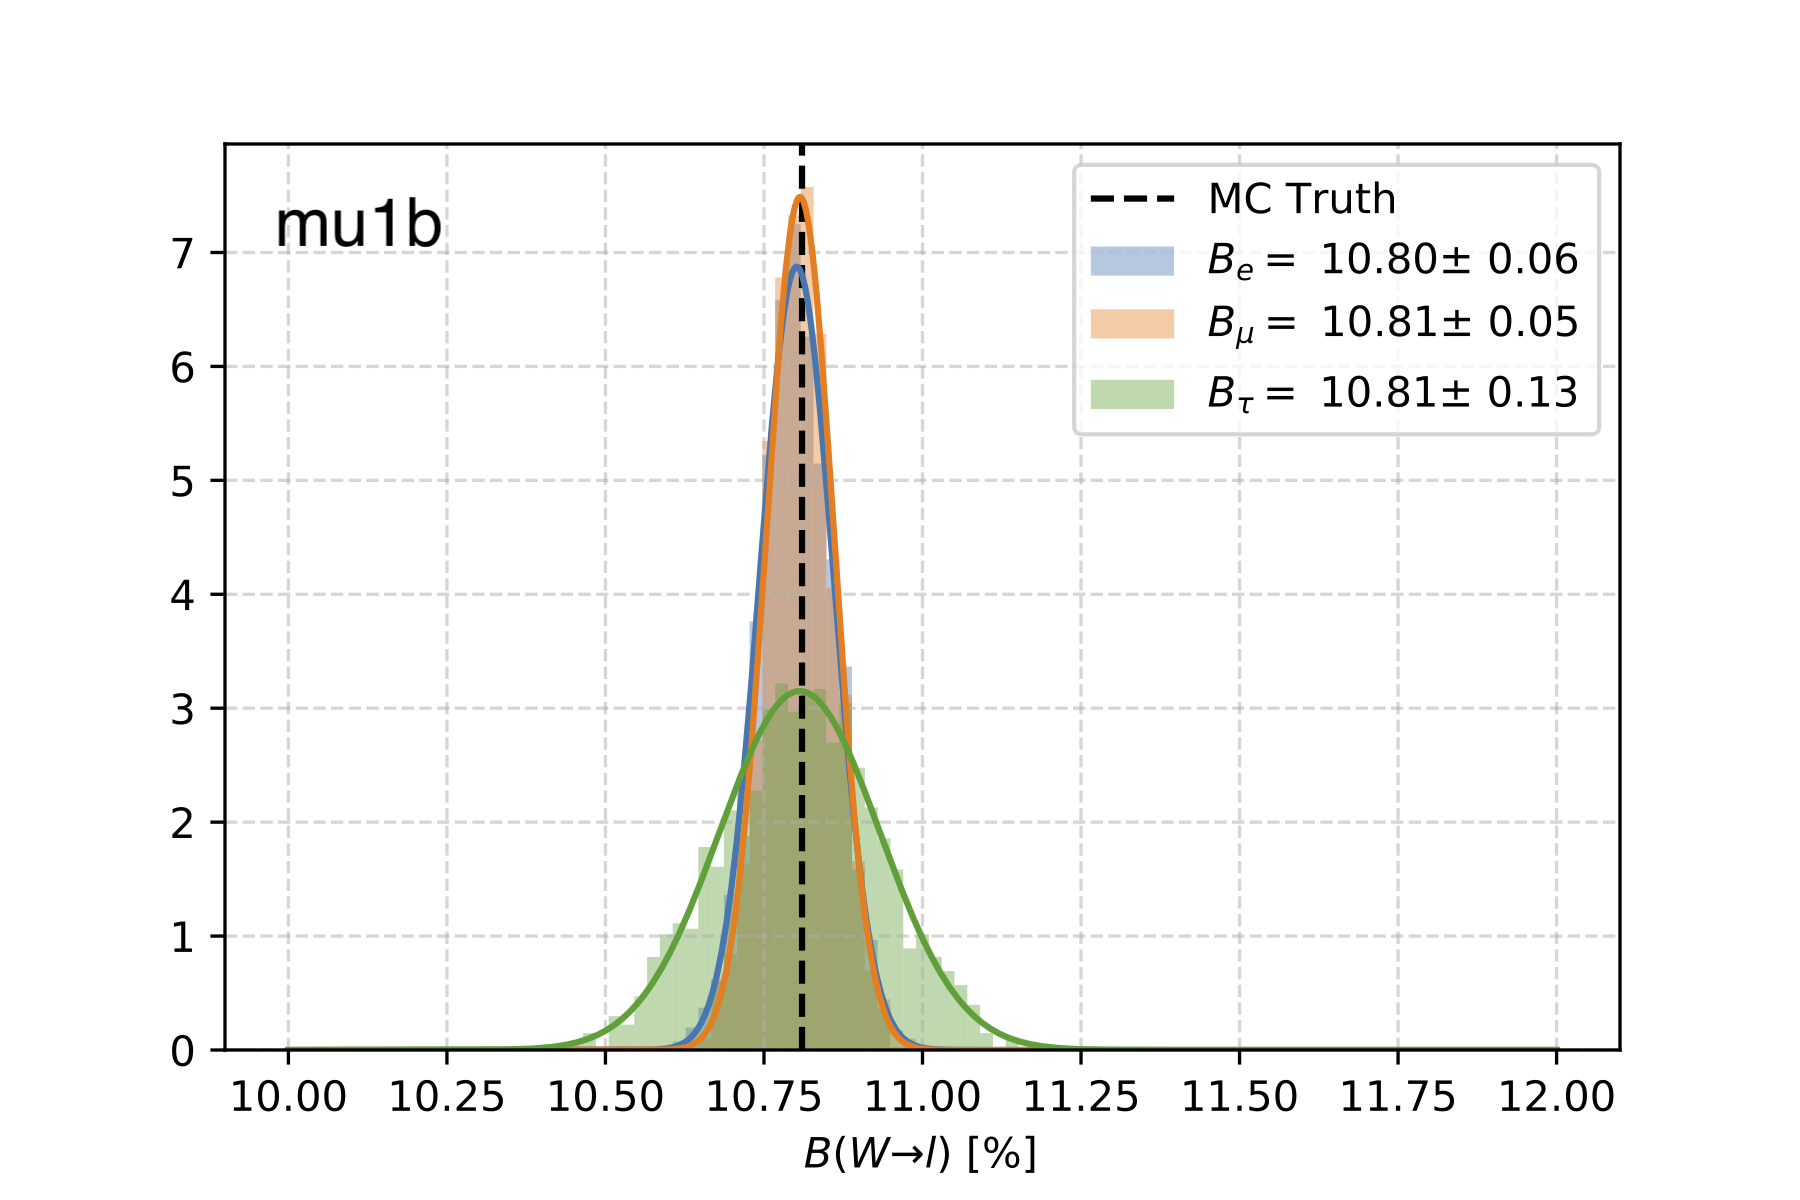
\includegraphics[width=7cm]{chapters/Analysis/sectionStatisticalAnalysis/figures/test_mu1b.png}
    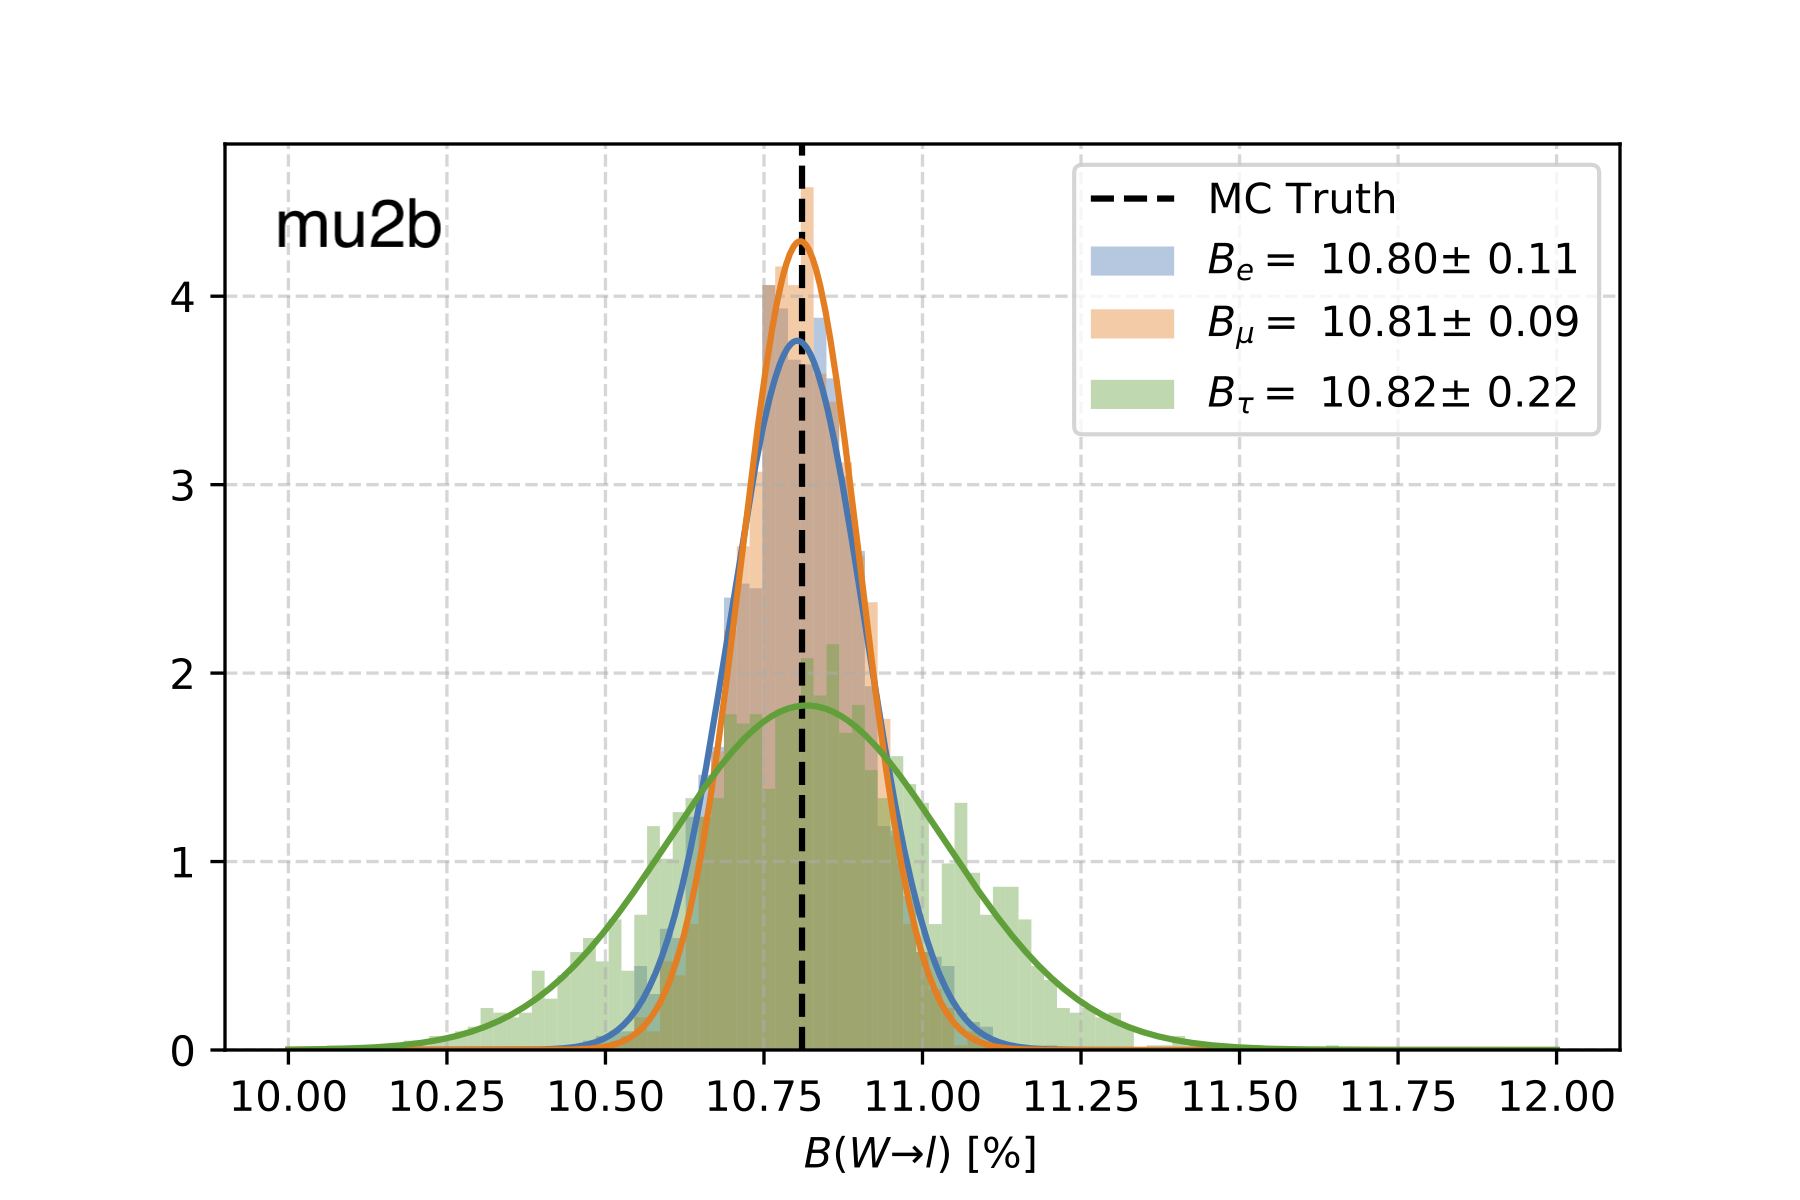
\includegraphics[width=7cm]{chapters/Analysis/sectionStatisticalAnalysis/figures/test_mu2b.png}
    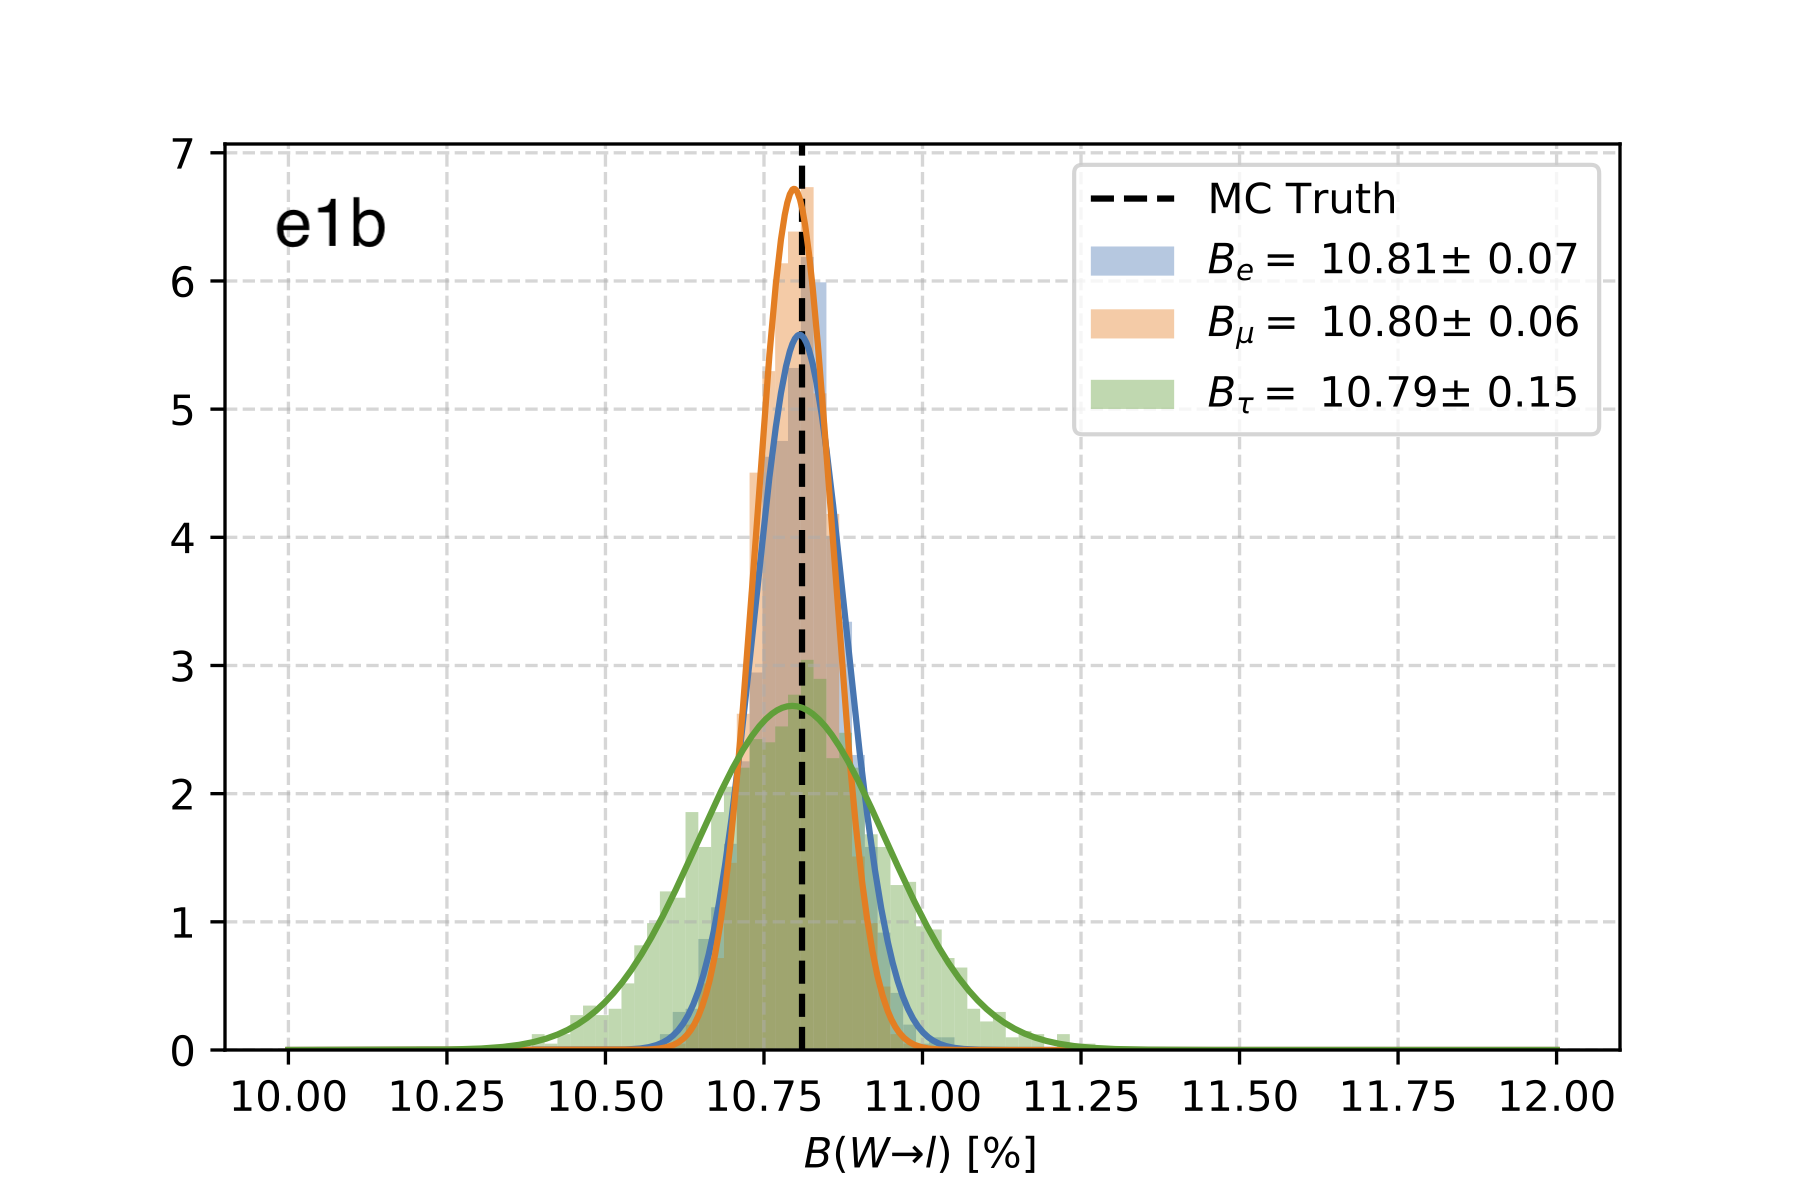
\includegraphics[width=7cm]{chapters/Analysis/sectionStatisticalAnalysis/figures/test_e1b.png}
    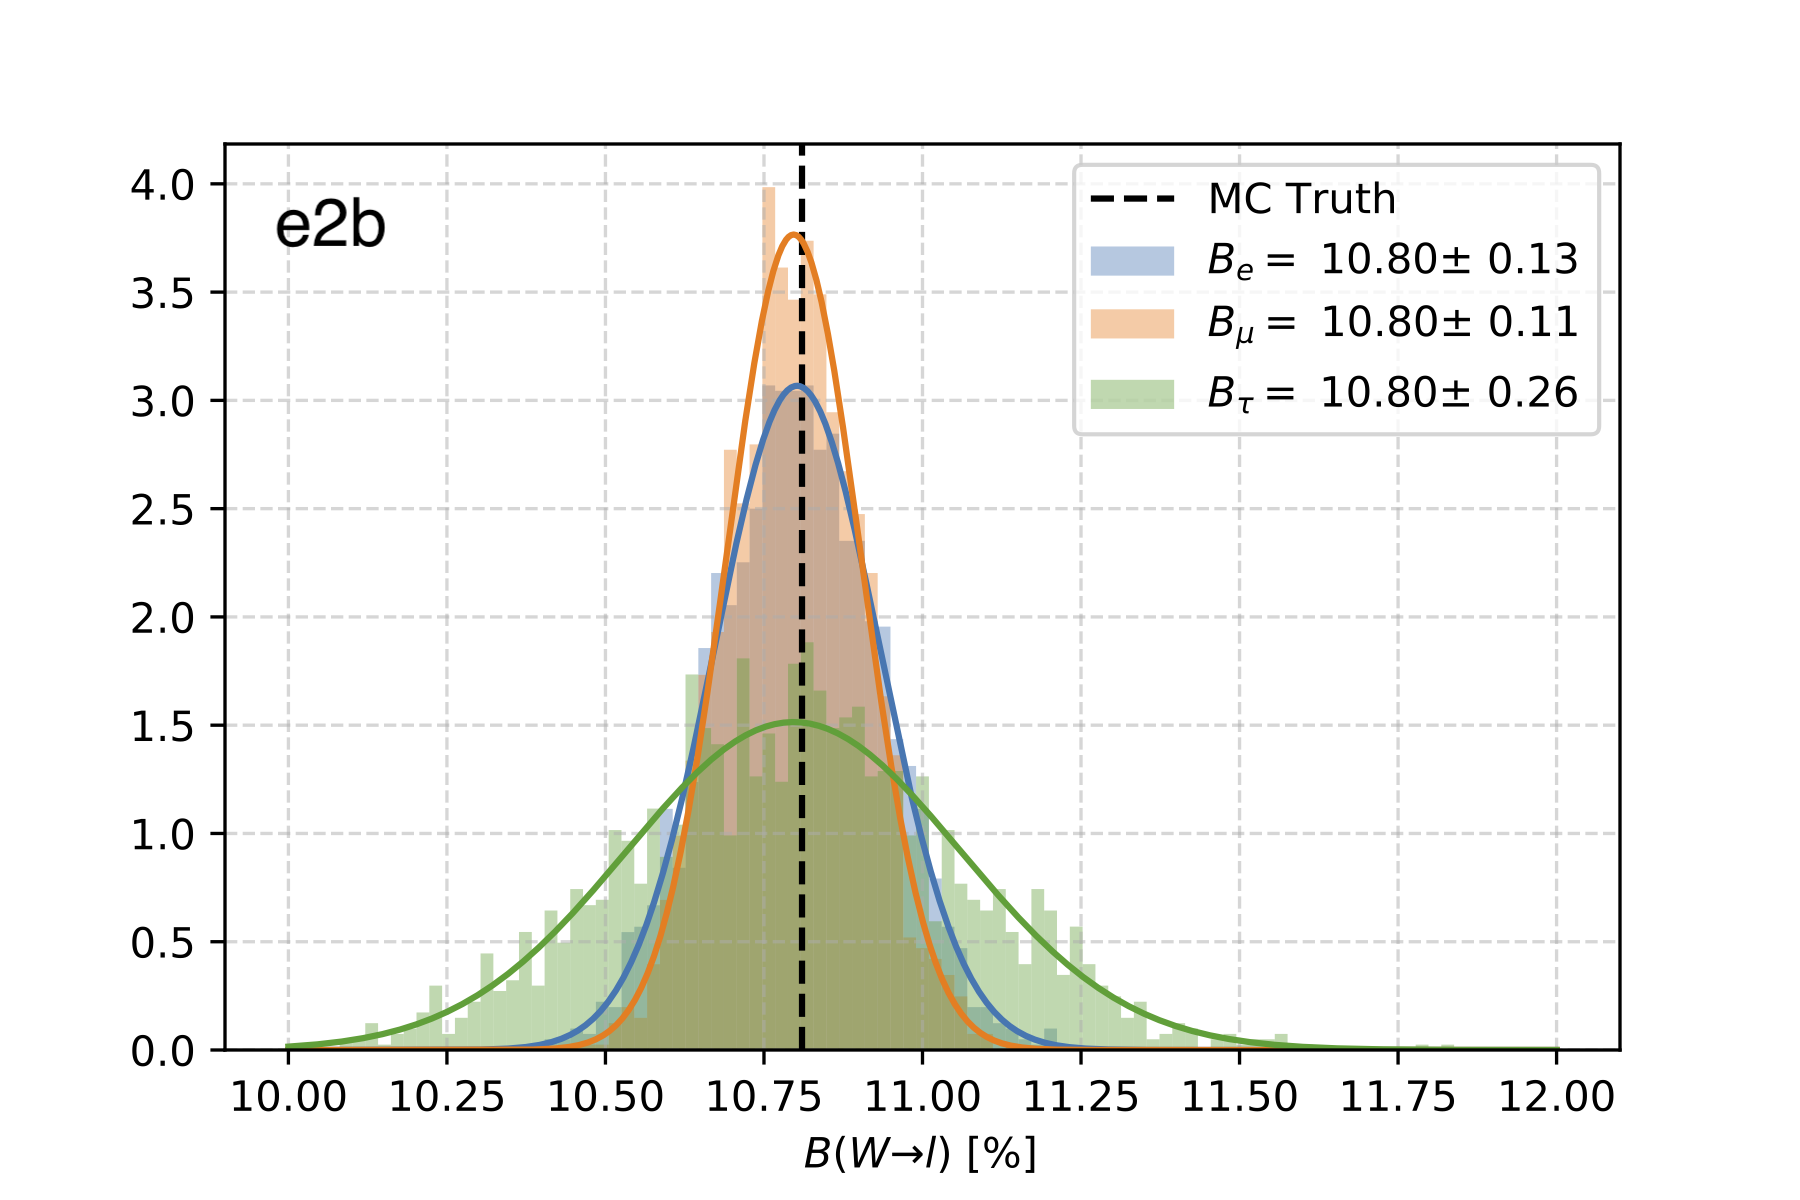
\includegraphics[width=7cm]{chapters/Analysis/sectionStatisticalAnalysis/figures/test_e2b.png}
    
    %--------------------------
    \caption{ Distribution of 2000 toys. }
    \label{fig:test_toy}
\end{figure}


\FloatBarrier


% %%%%%%%%%%%%%%%%%%%%%%%%%%%%%%%%%%%%%%%%
% % 2. Extraction of Parameters
% %%%%%%%%%%%%%%%%%%%%%%%%%%%%%%%%%%%%%%%%
% \subsection{Extraction of Parameters}

% In counting analysis, branching fractions are extracted by solving a set of
% three quadratic equations, obtained by setting the expected normalized
% yields equal to the measured ones. The four measurements are performed independently 
% in four mutually exclusive regions based on the number of b tags (1 or more than 2) 
% and trigger type (single electron or muon). Then these four measurements are combined based 
% on a $\chi^{2}$ minimization to obtain the final result.

% The four groups of channels and their yields
% are shown in figure~\ref{fig:signalRegion}.
% Channels using single-$\mu$ or single-$e$ trigger are

% \begin{itemize}
%     \item single-$\mu$ trigger : $\mu e$, $\mu\mu$, $\mu\tau$, $\mu h$.
%     \item single-$e$ trigger : $ee$, $e\mu$, $e\tau$, $eh$.
% \end{itemize}

% where $e\mu$ and $\mu e$ are mutually exclusive -- $e\mu$ channel
% requires fired e-trigger and $p^T_e > p^T_\mu$, while $\mu e$ channel
% requires fired $\mu$-trigger and $p^T_e < p^T_\mu$. 

% Besides being formally different from the shape analysis, the thresholds
% of leptons $p^T$ and working point for the hadronic tau isolation are
% slightly different, as optimizations in counting. This results in slightly different signal
% acceptances. For the 8 channels under consideration, the signal efficiency determined from
% simulated $t\bar{t}$ and tW events are shown in
% tables \ref{efficencyTableMuon} and \ref{efficencyTableElectron}. 
% The efficiency matrices \textbf{E} of 
% included channels in the four categories are shown in Fig \ref{efficencyMatrix}.



% The normalized yields, which are inspired by the definition of branching
% fraction, is the ratio of one yield over the sum of all yields in the
% trigger category:


% \begin{itemize}
%     \item single-$\mu$ trigger : 
%     $X_{e} = \frac{n^{\mu e}}{n^{\mu e} + n^{\mu \mu} + n^{\mu \tau} + n^{\mu h}}$, 
%     $X_{\mu} = \frac{n^{\mu \mu}}{n^{\mu e} + n^{\mu \mu} + n^{\mu \tau} + n^{\mu h}}$, 
%     $X_{\tau} = \frac{n^{\mu \tau}}{n^{\mu e} + n^{\mu \mu} + n^{\mu \tau} + n^{\mu h}}$,

%     \item single-$e$ trigger : 
%     $X_{e} = \frac{n^{e e}}{n^{e e} + n^{e \mu} + n^{e \tau} + n^{e h}}$, 
%     $X_{\mu} = \frac{n^{e \mu}}{n^{e e} + n^{e \mu} + n^{e \tau} + n^{e h}}$, 
%     $X_{\tau} = \frac{n^{e \tau}}{n^{e e} + n^{e \mu} + n^{e \tau} + n^{e h}}$,
% \end{itemize}

% where $n^f \equiv N^f - \sum_{k\in bg} N^f_k $ is the yield of channel
% $f$ with background subtracted. Based on Eqn \ref{eq:data_model}, the measured normalized yields
% $\{X_{e},X_{\mu},X_{\tau}\}$ should equal to the calculation with
% efficiency \textbf{E} and branching fraction \textbf{B}:

% \begin{equation} \label{quadEqA}
%     \begin{split}
%     X_e &= \frac{ E_{ij}^{te}B^{ij} }{E_{ij}^{te}B^{ij} + E_{ij}^{t\mu}B^{ij} + E_{ij}^{t\tau}B^{ij} + E_{ij}^{th}B^{ij}} \\
%     X_\mu &= \frac{ E_{ij}^{t\mu}B^{ij} }{E_{ij}^{te}B^{ij} + E_{ij}^{t\mu}B^{ij} + E_{ij}^{t\tau}B^{ij} + E_{ij}^{th}B^{ij}} \\
%     X_\tau &= \frac{ E_{ij}^{t\tau}B^{ij} }{E_{ij}^{te}B^{ij} + E_{ij}^{t\mu}B^{ij} + E_{ij}^{t\tau}B^{ij} + E_{ij}^{th}B^{ij}}
%     \end{split}
% \end{equation}



% % where $n^f \equiv N^f - \sum_{k\in bg} n^f_k $ is the yield of channel $f$ 
% % with background subtracted and three normalized yields, 
% % $\{r_{e},r_{\mu},r_{\tau}\}$, are measured from data with background subtracted. 

% % Based on Eqn \ref{prediction}, the measured normalized yields $\{r_{e},r_{\mu},r_{\tau}\}$ 
% % should equal to the calculation with efficiency \textbf{E} and branching fraction \textbf{B}:




% where $t\in \{\mu,e\}$ depends on the trigger category. Plugging in
% explicit form of \textbf{E} and \textbf{B} matrices in Eqn \ref{eq:br_matrix} and Eqn \ref{eq:eff_matrix}
% and unity condition of branching fraction $\beta_h = 1- \beta_e -
% \beta_\mu - \beta_\tau$, Eq \ref{quadEqA} can be written as a set of
% three quadratic equations with
% $\{\beta_{e},\beta_{\mu},\beta_{\tau}\}$ as three unknowns.


% \begin{equation} \label{quadEqB}
%     \footnotesize
% 	\begin{split}
%         Q_e(\beta_e,\beta_\mu,\beta_\tau) &=
%         c_{e1} \beta_e^2 + c_{e2} \beta_\mu^2 + c_{e3} \beta_\tau^2 + 
%         c_{e4} \beta_e\beta_\mu + c_{e5} \beta_e\beta_\tau + c_{e6} \beta_\mu\beta_\tau +
%         c_{e7} \beta_e + c_{e8} \beta_\mu + c_{e9} \beta_\tau + c_{e0} = 0 \\
%         %
%         Q_\mu(\beta_e,\beta_\mu,\beta_\tau) &= 
%         c_{\mu 1} \beta_e^2 + c_{\mu 2} \beta_\mu^2 + c_{\mu 3} \beta_\tau^2 + 
%         c_{\mu 4} \beta_e\beta_\mu + c_{\mu 5} \beta_e\beta_\tau + c_{\mu 6} \beta_\mu\beta_\tau +
%         c_{\mu 7} \beta_e + c_{\mu 8} \beta_\mu + c_{\mu 9} \beta_\tau + c_{\mu 0} = 0 \\
%         %
%         Q_\tau(\beta_e,\beta_\mu,\beta_\tau) &= 
%         c_{_\tau1} \beta_e^2 + c_{\tau2} \beta_\mu^2 + c_{\tau3} \beta_\tau^2 + 
%         c_{\tau4} \beta_e\beta_\mu + c_{\tau5} \beta_e\beta_\tau + c_{\tau6} \beta_\mu\beta_\tau +
%         c_{\tau7} \beta_e + c_{\tau8} \beta_\mu + c_{\tau9} \beta_\tau + c_{\tau0} = 0 
%     \end{split}
% \end{equation}

% where coefficients $c_{ei},c_{\mu i},c_{\tau i}$ are fully determined 
% by efficiency \textbf{E} and normalized yields $\{X_{e},X_{\mu},X_{\tau}\}$,
% as are listed in table~\ref{quadcoeff}.

% \begin{table}[ht]
    \centering
   	\setlength{\tabcolsep}{0.4em}
    \renewcommand{\arraystretch}{1.5}
    \small
    
    \begin{tabular}{c|l}

    \hline
    $c_{l0}$ & $\Delta_{hh}$ \\
    \hline
    $c_{l1}$ & $\Delta_{ee}     - 2\Delta_{eh}   + \Delta_{hh}$ \\
    \hline
    $c_{l2}$ & $\Delta_{\mu\mu} - 2\Delta_{\mu h} + \Delta_{hh}$ \\
    \hline
    
    $c_{l3}$ & $   b^\tau_e   b^\tau_e   \Delta_{\tau_e   \tau_e}  
    			 + b^\tau_\mu b^\tau_\mu \Delta_{\tau_\mu \tau_\mu}
                 + b^\tau_h   b^\tau_h   \Delta_{\tau_h   \tau_h}
                 
                 + 2 b^\tau_e   b^\tau_\mu \Delta_{\tau_e   \tau_\mu} 
    		     + 2 b^\tau_e   b^\tau_h   \Delta_{\tau_e   \tau_h}   
    		     + 2 b^\tau_\mu b^\tau_h   \Delta_{\tau_\mu \tau_h} - $ \\
                 
             & $   2 b^\tau_e   \Delta_{e   \tau_h}
                 - 2 b^\tau_\mu \Delta_{\mu \tau_h}
                 - 2 b^\tau_h   \Delta_{h.  \tau_h} 
                 + \Delta_{hh} $ \\

    \hline
    $c_{l4}$ & $2\Delta_{e\mu} - 2\Delta_{eh} -2\Delta_{\mu h} +2\Delta_{hh}$  \\
    \hline
    $c_{l5}$ & $  2b^\tau_e   \Delta_{e \tau_e} 
    			+ 2b^\tau_\mu \Delta_{e \tau_\mu}
                + 2b^\tau_h   \Delta_{e \tau_h}
                - 2b^\tau_e   \Delta_{\tau_e   h} 
    			- 2b^\tau_\mu \Delta_{\tau_\mu h}
                - 2b^\tau_h   \Delta_{\tau_h   h} 
                - 2\Delta_{eh}   + 2 \Delta_{hh} $ \\
        
    \hline            
    $c_{l6}$ & $  2b^\tau_e   \Delta_{\mu \tau_e} 
    			+ 2b^\tau_\mu \Delta_{\mu \tau_\mu}
                + 2b^\tau_h   \Delta_{\mu \tau_h}
                - 2b^\tau_e   \Delta_{\tau_e   h} 
    			- 2b^\tau_\mu \Delta_{\tau_\mu h}
                - 2b^\tau_h   \Delta_{\tau_h   h} 
                - 2\Delta_{\mu h}   + 2 \Delta_{hh} $ \\
    \hline            
    $c_{l7}$ & $ 2\Delta_{eh}      - 2 \Delta_{hh} $ \\
    \hline
    $c_{l8}$ & $ 2\Delta_{\mu h}   - 2 \Delta_{hh}$ \\
    \hline
    $c_{l9}$ & $  2b^\tau_e   \Delta_{\tau_e   h} 
                 + 2b^\tau_\mu \Delta_{\tau_\mu h} 
                 + 2b^\tau_h   \Delta_{\tau_h   h} 
                 - 2 \Delta_{hh}$ \\
    \hline
    \hline
    where  & $ \Delta \equiv E^{tl} - X_l \times ( E^{te} + E^{t\mu} + E^{t\tau} + E^{th} )$ \\
           & $l=e,\mu,\tau$ and $t=e(\mu)$ if using single-$e$ (signle-$\mu$) trigger\\
    \hline
    
	\end{tabular}
    
\caption{ Coefficients of quadratic equations in terms of E and X. In the table, $l=e,\mu,\tau$ and $t=\mu,e$ for single-$\mu$ and single-$e$ trigger respectively.  }
\label{quadcoeff}
    
\end{table}


% In the $\{\beta_{e},\beta_{\mu},\beta_{\tau}\}$ parameter space, 
% equation~\ref{quadEqB} represents three hyperbolic planes, intersection 
% of which is the solution of desired branching fractions, as is shown
% in figure~\ref{visualize}.


% \begin{figure}[ht]
%     \centering
%     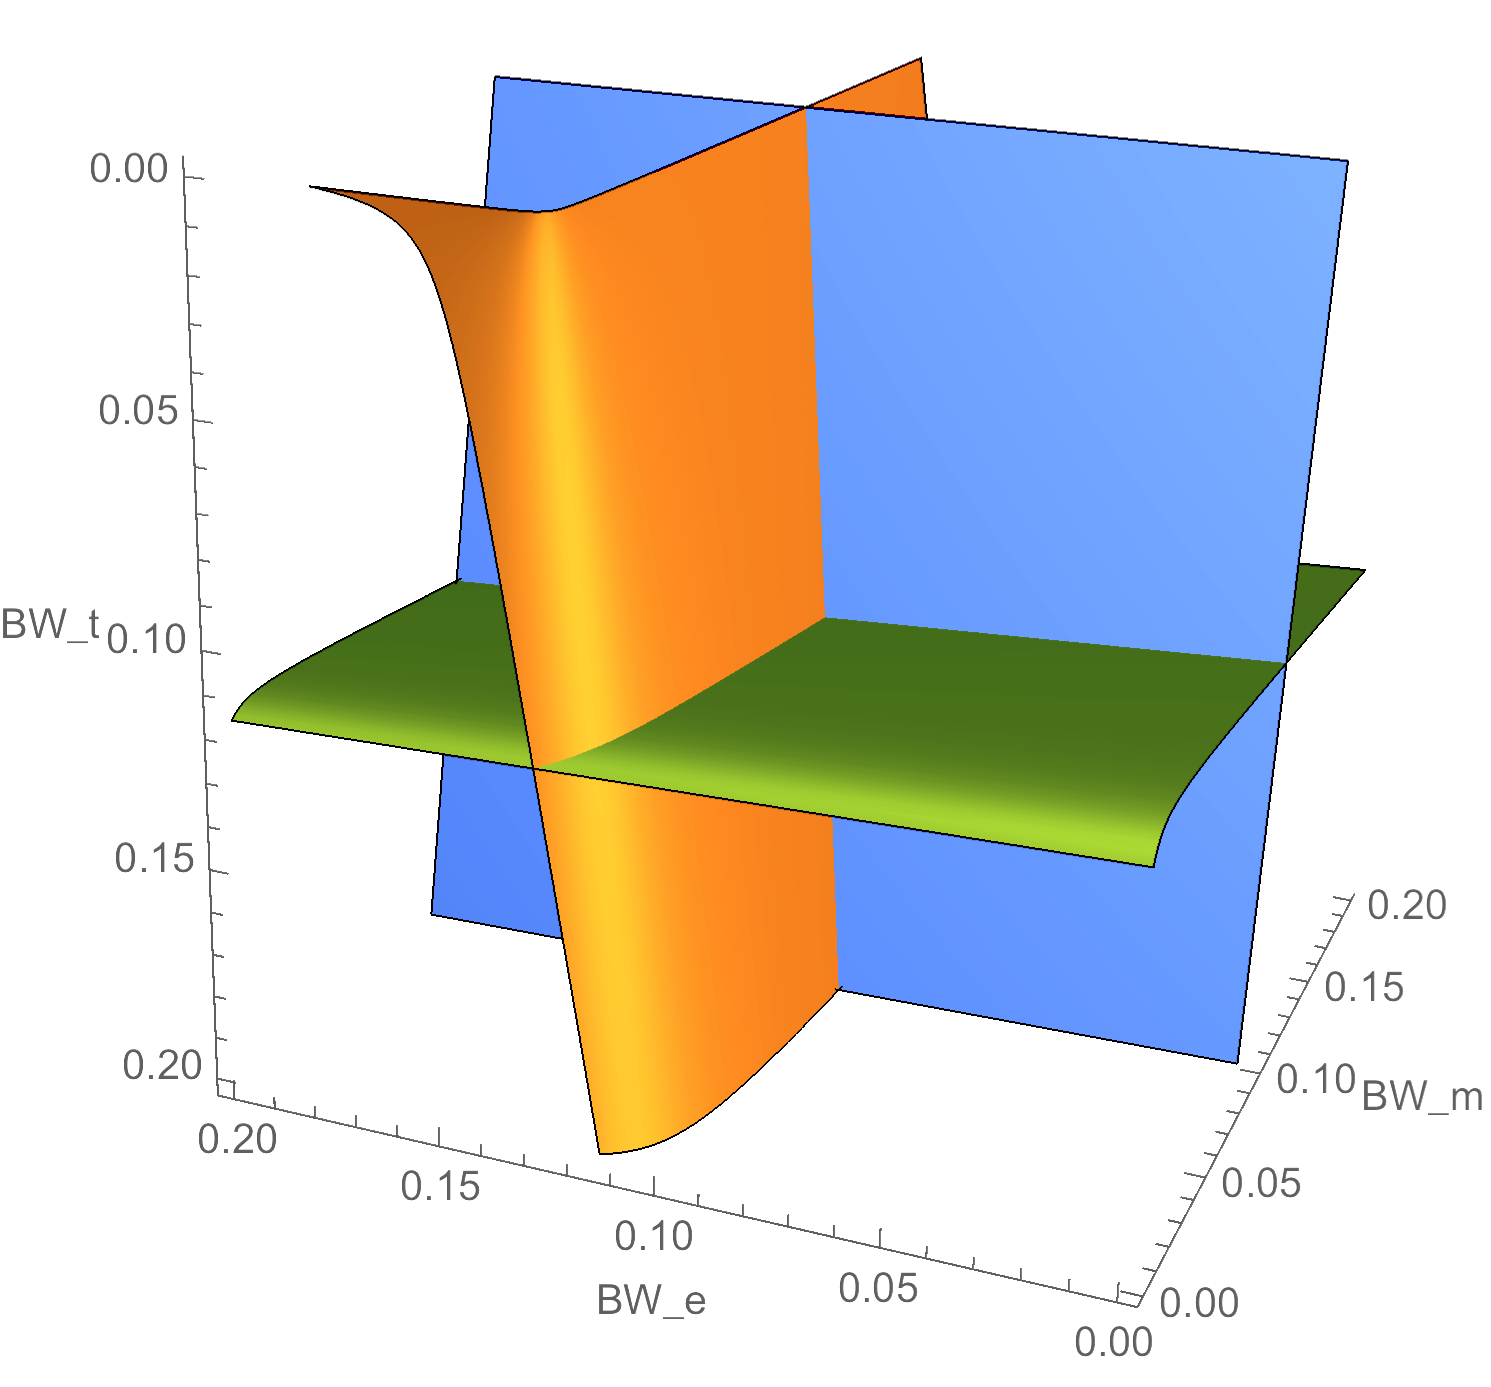
\includegraphics[width=7cm]{chapters/Analysis/sectionStatisticalAnalysis/figures/visual.png}
    
%     %--------------------------
%     \caption{Visualization of Eq \ref{quadEqB} in the
%     $\{\beta_{e},\beta_{\mu},\beta_{\tau}\}$ parameter space. Each
%     equation in Eq \ref{quadEqB} is a hyperbolic plane, while their
%     intersection is the solution Eq \ref{quadEqB}. Mathematically, there
%     are 8 possible solutions. However, only one solution is physical,
%     located with $\beta \in (0,1) $. }
%     \label{visualize}
% \end{figure}

% % This approach analytically obtains the coefficient $c_{ij}$ in 
% % Eq \ref{quadEqB} from efficiency matrix \textbf{E} and measured 
% % normalized yields $\{X_{e},X_{\mu},X_{\tau}\}$. Then it numerically
% % solves the branching fractions $\{\beta_{e},\beta_{\mu},\beta_{\tau}\}$,
% % using a modification of the Powell hybrid method as implemented in MINPACK-Scipy. 

% \begin{equation} 
%     \left [
%     \begin{tabular}{c}
% 	    $\beta_{e}$ \\
% 	    $\beta_{\mu}$ \\
% 	    $\beta_{\tau}$
%     \end{tabular}
%     \right ]
%     = Solution
%     \left [
%     \begin{tabular}{c}
% 	    $Q_e    (\beta_e,\beta_\mu,\beta_\tau) = 0$ \\
% 	    $Q_\mu  (\beta_e,\beta_\mu,\beta_\tau) = 0$ \\
% 	    $Q_\tau (\beta_e,\beta_\mu,\beta_\tau) = 0$
%     \end{tabular}
% \right ]
% \end{equation}

% \FloatBarrier

%%%%%%%%%%%%%%%%%%%%%%%%%%%%%%%%%%%%%%%%
% 3. Test of Parameters Extraction
%%%%%%%%%%%%%%%%%%%%%%%%%%%%%%%%%%%%%%%%
% \subsection{Test of Parameters Extraction}






% \begin{quote}
    
%     After establishing parameter extraction, we perform a closure test using 
%     signal MC samples. As is described above, the input of parameter extraction 
%     is data yields with background subtracted $n=N_{data} - N_{mc,bg}$. 
%     But here for testing purpose, we replace $n=N_{data} - N_{mc,bg}$ with $N_{mc,sg}$ as the input,
%     as is given in Eqn \ref{eqn:testinput}.
%     The pass of the test is that parameter extraction 
%     gives back branching fraction assumed in the MC generator, which is $10.80\%$.
    
    
%     \begin{equation}
%     	n=N_{mc,sg}\pm \sqrt{N_{mc,sg}}
%     	\label{eqn:testinput}
%     \end{equation}
    
%     where $N_{mc,sg}$ comes from tt and tW MC sample normalized to luminosity. 
%     It is uncertainty is assumed as a Gaussian error with width $\sqrt{N_{sg}}$, 
%     so as to estimate the expected statistical uncertainty of data.
%     The extracted branching fraction is listed in Table \ref{test_ana}.

% \end{quote}



% \begin{table}[ht]
%     \centering
% 	\begin{tabular}{l|ccc}
%     \hline
%           	 & $\beta_e$             &   $\beta_\mu$       	 & 	  $\beta_\tau$   	 \\
%     MC Assumption  & 10.80 		 &  10.80 		 	 & 	  10.80     	 \\
%     \hline
%   	$\mu-1b$ &   10.802$\pm$0.058  &   10.807$\pm$0.053  &    10.808$\pm$0.127 \\
%   	$\mu-2b$ &   10.802$\pm$0.103  &   10.807$\pm$0.092  &    10.808$\pm$0.216 \\
%   	$e-1b$   &   10.804$\pm$0.073  &   10.797$\pm$0.059  &    10.794$\pm$0.152 \\
%   	$e-2b$   &   10.805$\pm$0.130  &   10.797$\pm$0.104  &    10.794$\pm$0.263 \\
%     \hline
% 	\end{tabular}
	
% 	%--------------------------
%     \caption{Branching fraction extracted from signal MC. The 
%     uncertainty is calculated by error propagation. The small 
%     deviation from MC assumption is resulted by the difference 
%     value of $Br(\tau \to e)$ and $Br(\tau \to \mu)$ in MC and in 
%     extractor. The extractor uses 0.1773,0.1731 respectively, while 
%     the MC assumption of tau decay needs to be found in generator 
%     cards. 
%     }
%     \label{test_ana}
% \end{table}



% In addition, to test the error propagation, we generate 2000 toy experiments, 
% each of which variates the yield $n=N_{sg}$ by $\sqrt{N_{sg}}$.
% The width of distribution of toys is consistent with uncertainty 
% from error propagation list in the Table \ref{test_ana}.
% Also as expected, the center of distribution of toys is consistent with
% the assumed branching fraction in the MC generator.






% Finally, the branching fractions obtained in all four categories are combined:

% \begin{equation}
% 	\beta_i = \frac{ \sum_{cat} \beta_i^{cat} / \sigma^2_{\beta_i^{cat}}}{\sum_{cat} 1 / \sigma^2_{\beta_i^{cat}}} ,
%     \qquad
%     \sigma^2_{\beta_i} = \frac{1}{\sum_{cat} 1 / \sigma^2_{\beta_i^{cat}} }
% \end{equation}

% where $i = e,\mu,\tau$ and categories are single electron or muon trigger with 1 or 2 b-jets, $cat \in \{\mu \text{-} 1b,\mu \text{-} 2b,e \text{-} 1b,e \text{-} 2b \}$

